% !TeX encoding = UTF-8
% !TeX program = xelatex
% !TeX spellcheck = en_US

\documentclass[degree=master]{thuthesis}
  % 学位 degree:
  %   doctor | master | bachelor | postdoc
  % 学位类型 degree-type:
  %   academic(默认)| professional
  % 语言 language
  %   chinese(默认)| english
  % 字体库 fontset
  %   windows | mac | fandol | ubuntu
  % 建议终版使用 Windows 平台的字体编译


% 论文基本配置,加载宏包等全局配置
% !TeX root = ./PhDThesis.tex

% 论文基本信息配置

\thusetup{
  %******************************
  % 注意:
  %   1. 配置里面不要出现空行
  %   2. 不需要的配置信息可以删除
  %   3. 建议先阅读文档中所有关于选项的说明
  %******************************
  %
  % 输出格式
  %   选择打印版(print)或用于提交的电子版(electronic),前者会插入空白页以便直接双面打印
  %
  output = print,
  %
  % 书写语言
  %
  language = english,
  %
  % 标题
  %   可使用“\\”命令手动控制换行
  %
  title  = {用于多比特量子存储器的低温离子阱系统},
  title* = {Cryogenic Trapped-Ion System for Multiqubit Quantum Memory},
  %
  % 学位
  %   1. 学术型
  %      - 中文
  %        需注明所属的学科门类,例如:
  %        哲学、经济学、法学、教育学、文学、历史学、理学、工学、农学、医学、
  %        军事学、管理学、艺术学
  %      - 英文
  %        博士:Doctor of Philosophy
  %        硕士:
  %          哲学、文学、历史学、法学、教育学、艺术学门类,公共管理学科
  %          填写“Master of Arts“,其它填写“Master of Science”
  %   2. 专业型
  %      直接填写专业学位的名称,例如:
  %      教育博士、工程硕士等
  %      Doctor of Education, Master of Engineering
  %   3. 本科生不需要填写
  %
  degree-name  = {理学博士},
  degree-name* = {Doctor of Philosophy},
  %
  % 培养单位
  %   填写所属院系的全名
  %
  department = {交叉信息研究院},
  %
  % 学科
  %   1. 学术型学位
  %      获得一级学科授权的学科填写一级学科名称,其他填写二级学科名称
  %   2. 工程硕士
  %      工程领域名称
  %   3. 其他专业型学位
  %      不填写此项
  %   4. 本科生填写专业名称,第二学位论文需标注“(第二学位)”
  %
  discipline  = {物理学},
  discipline* = {Physics},
  %
  % 姓名
  %
  author  = {姚睿},
  author* = {Yao Rui},
  %
  % 指导教师
  %   中文姓名和职称之间以英文逗号“,”分开,下同
  %
  supervisor  = {段路明, 教授},
  supervisor* = {Professor Luming Duan},
  %
  % 副指导教师
  %
  % associate-supervisor  = {某某某, 教授},
  % associate-supervisor* = {Professor},
  %
  % 联合指导教师
  %
  % co-supervisor  = {某某某, 教授},
  % co-supervisor* = {Professor Mou Moumou},
  %
  % 日期
  %   使用 ISO 格式;默认为当前时间
  %
  % date = {2019-07-07},
  %
  % 是否在中文封面后的空白页生成书脊(默认 false)
  %
  include-spine = false,
  %
  % 密级和年限
  %   秘密, 机密, 绝密
  %
  % secret-level = {秘密},
  % secret-year  = {10},
  %
  % 博士后专有部分
  %
  % clc                = {分类号},
  % udc                = {UDC},
  % id                 = {编号},
  % discipline-level-1 = {计算机科学与技术},  % 流动站(一级学科)名称
  % discipline-level-2 = {系统结构},          % 专业(二级学科)名称
  % start-date         = {2011-07-01},        % 研究工作起始时间
}

% 载入所需的宏包

% 定理类环境宏包
\usepackage{amsthm}
% 也可以使用 ntheorem
% \usepackage[amsmath,thmmarks,hyperref]{ntheorem}

\thusetup{
  %
  % 数学字体
  % math-style = GB,  % GB | ISO | TeX
  math-font  = xits,  % stix | xits | libertinus
}

% 可以使用 nomencl 生成符号和缩略语说明
\usepackage{nomencl}
\makenomenclature

% 表格加脚注
\usepackage{threeparttable}

% 表格中支持跨行
\usepackage{multirow}

% 固定宽度的表格。
% \usepackage{tabularx}

% 跨页表格
\usepackage{longtable}

% 算法
\usepackage{algorithm}
\usepackage{algorithmic}

% 量和单位
\usepackage{siunitx}

% 参考文献使用 BibTeX + natbib 宏包
% 顺序编码制
\usepackage[sort]{natbib}
\bibliographystyle{thuthesis-numeric}

% 著者-出版年制
% \usepackage{natbib}
% \bibliographystyle{thuthesis-author-year}

% 本科生参考文献的著录格式
% \usepackage[sort]{natbib}
% \bibliographystyle{thuthesis-bachelor}

% 参考文献使用 BibLaTeX 宏包
% \usepackage[style=thuthesis-numeric]{biblatex}
% \usepackage[style=thuthesis-author-year]{biblatex}
% \usepackage[style=apa]{biblatex}
% \usepackage[style=mla-new]{biblatex}
% 声明 BibLaTeX 的数据库
% \addbibresource{ref/refs.bib}

% 定义所有的图片文件在 figures 子目录下
\graphicspath{{figures/}}

% 数学命令
\makeatletter
\newcommand\dif{%  % 微分符号
  \mathop{}\!%
  \ifthu@math@style@TeX
    d%
  \else
    \mathrm{d}%
  \fi
}
\makeatother

% hyperref 宏包在最后调用
\usepackage{hyperref}



\begin{document}

% 封面
\maketitle

% 学位论文指导小组、公开评阅人和答辩委员会名单
% 本科生不需要
% !TeX root = ./PhDThesis.tex

\begin{committee}[name={学位论文指导小组、公开评阅人和答辩委员会名单}]

  \newcolumntype{C}[1]{@{}>{\centering\arraybackslash}p{#1}}

  % \section*{指导小组名单}

  % \begin{center}
  %   \begin{tabular}{C{3cm}C{3cm}C{9cm}@{}}
  %     段路明 & 教授 & 清华大学 \\
  %   \end{tabular}
  % \end{center}


  % \section*{公开评阅人名单}

  % \begin{center}
  %   \begin{tabular}{C{3cm}C{3cm}C{9cm}@{}}
  %     刘XX & 教授  & 清华大学                \\
  %     陈XX & 副教授 & XXXX大学              \\
  %     杨XX & 研究员 & 中国XXXX科学院XXXXXXX研究所 \\
  %   \end{tabular}
  % \end{center}


  \section*{答辩委员会名单}

  \begin{center}
    \begin{tabular}{C{2.75cm}C{2.98cm}C{4.63cm}C{4.63cm}@{}}
      主席 & 范桁  & 研究员  & 中国科学院物理研究所 \\
      委员 & 段路明 & 教授   & 清华大学       \\
      % & \multirow{2}{*}{杨XX} & \multirow{2}{*}{研究员} & 中国XXXX科学院 \\
      % &                       &                         & XXXXXXX研究所  \\
         & 孙麓岩 & 副教授  & 清华大学       \\
         & 吴宇恺 & 助理教授 & 清华大学       \\
         & 孙栋  & 副教授  & 北京大学       \\
         & 张威  & 教授   & 中国人民大学     \\
      秘书 & 姜越  & 博士后  & 清华大学       \\
    \end{tabular}
  \end{center}
\end{committee}



% 也可以导入 Word 版转的 PDF 文件
% \begin{committee}[file=figures/committee.pdf]
% \end{committee}


% 使用授权的说明
\copyrightpage
% 将签字扫描后授权文件 scan-copyright.pdf 替换原始页面
% \copyrightpage[file=scan-copyright.pdf]

\frontmatter
% !TeX root = ./PhDThesis.tex

% 中英文摘要和关键字

\begin{abstract}
  论文的摘要是对论文研究内容和成果的高度概括21。
  摘要应对论文所研究的问题及其研究目的进行描述,对研究方法和过程进行简单介绍,对研究成果和所得结论进行概括。
  摘要应具有独立性和自明性,其内容应包含与论文全文同等量的主要信息。
  使读者即使不阅读全文,通过摘要就能了解论文的总体内容和主要成果。

  论文摘要的书写应力求精确、简明。
  切忌写成对论文书写内容进行提要的形式,尤其要避免“第 1 章……;第 2 章……;……”这种或类似的陈述方式。

  关键词是为了文献标引工作、用以表示全文主要内容信息的单词或术语。
  关键词不超过 5 个,每个关键词中间用分号分隔。

  % 关键词用“英文逗号”分隔,输出时会自动处理为正确的分隔符
  \thusetup{
    keywords = {关键词 1, 关键词 2, 关键词 3, 关键词 4, 关键词 5},
  }
\end{abstract}

\begin{abstract*}
  An abstract of a dissertation is a summary and extraction of research work and contributions.
  Included in an abstract should be description of research topic and research objective, brief introduction to methodology and research process, and summary of conclusion and contributions of the research.
  An abstract should be characterized by independence and clarity and carry identical information with the dissertation.
  It should be such that the general idea and major contributions of the dissertation are conveyed without reading the dissertation.

  An abstract should be concise and to the point.
  It is a misunderstanding to make an abstract an outline of the dissertation and words “the first chapter”, “the second chapter” and the like should be avoided in the abstract.

  Keywords are terms used in a dissertation for indexing, reflecting core information of the dissertation.
  An abstract may contain a maximum of 5 keywords, with semi-colons used in between to separate one another.

  % Use comma as separator when inputting
  \thusetup{
    keywords* = {keyword 1, keyword 2, keyword 3, keyword 4, keyword 5},
  }
\end{abstract*}


% 目录
\tableofcontents

% 插图和附表清单
% 本科生的插图索引和表格索引需要移至正文之后、参考文献前
% \listoffiguresandtables  % 插图和附表清单(仅限研究生)
\listoffigures           % 插图清单
\listoftables            % 附表清单

% 符号对照表
% !TeX root = ../thuthesis-example.tex

\begin{denotation}[3cm]
  \item[PI] 聚酰亚胺
  \item[MPI] 聚酰亚胺模型化合物,N-苯基邻苯酰亚胺
  \item[PBI] 聚苯并咪唑
  \item[MPBI] 聚苯并咪唑模型化合物,N-苯基苯并咪唑
  \item[PY] 聚吡咙
  \item[PMDA-BDA] 均苯四酸二酐与联苯四胺合成的聚吡咙薄膜
  \item[MPY] 聚吡咙模型化合物
  \item[As-PPT] 聚苯基不对称三嗪
  \item[MAsPPT] 聚苯基不对称三嗪单模型化合物,3,5,6-三苯基-1,2,4-三嗪
  \item[DMAsPPT] 聚苯基不对称三嗪双模型化合物(水解实验模型化合物)
  \item[S-PPT] 聚苯基对称三嗪
  \item[MSPPT] 聚苯基对称三嗪模型化合物,2,4,6-三苯基-1,3,5-三嗪
  \item[PPQ] 聚苯基喹噁啉
  \item[MPPQ] 聚苯基喹噁啉模型化合物,3,4-二苯基苯并二嗪
  \item[HMPI] 聚酰亚胺模型化合物的质子化产物
  \item[HMPY] 聚吡咙模型化合物的质子化产物
  \item[HMPBI] 聚苯并咪唑模型化合物的质子化产物
  \item[HMAsPPT] 聚苯基不对称三嗪模型化合物的质子化产物
  \item[HMSPPT] 聚苯基对称三嗪模型化合物的质子化产物
  \item[HMPPQ] 聚苯基喹噁啉模型化合物的质子化产物
  \item[PDT] 热分解温度
  \item[HPLC] 高效液相色谱(High Performance Liquid Chromatography)
  \item[HPCE] 高效毛细管电泳色谱(High Performance Capillary lectrophoresis)
  \item[LC-MS] 液相色谱-质谱联用(Liquid chromatography-Mass Spectrum)
  \item[TIC] 总离子浓度(Total Ion Content)
  \item[\textit{ab initio}] 基于第一原理的量子化学计算方法,常称从头算法
  \item[DFT] 密度泛函理论(Density Functional Theory)
  \item[$E_a$] 化学反应的活化能(Activation Energy)
  \item[ZPE] 零点振动能(Zero Vibration Energy)
  \item[PES] 势能面(Potential Energy Surface)
  \item[TS] 过渡态(Transition State)
  \item[TST] 过渡态理论(Transition State Theory)
  \item[$\increment G^\neq$] 活化自由能(Activation Free Energy)
  \item[$\kappa$] 传输系数(Transmission Coefficient)
  \item[IRC] 内禀反应坐标(Intrinsic Reaction Coordinates)
  \item[$\nu_i$] 虚频(Imaginary Frequency)
  \item[ONIOM] 分层算法(Our own N-layered Integrated molecular Orbital and molecular Mechanics)
  \item[SCF] 自洽场(Self-Consistent Field)
  \item[SCRF] 自洽反应场(Self-Consistent Reaction Field)
\end{denotation}



% 也可以使用 nomencl 宏包,需要在导言区
% \usepackage{nomencl}
% \makenomenclature

% 在这里输出符号说明
% \printnomenclature[3cm]

% 在正文中的任意为都可以标题
% \nomenclature{PI}{聚酰亚胺}
% \nomenclature{MPI}{聚酰亚胺模型化合物,N-苯基邻苯酰亚胺}
% \nomenclature{PBI}{聚苯并咪唑}
% \nomenclature{MPBI}{聚苯并咪唑模型化合物,N-苯基苯并咪唑}
% \nomenclature{PY}{聚吡咙}
% \nomenclature{PMDA-BDA}{均苯四酸二酐与联苯四胺合成的聚吡咙薄膜}
% \nomenclature{MPY}{聚吡咙模型化合物}
% \nomenclature{As-PPT}{聚苯基不对称三嗪}
% \nomenclature{MAsPPT}{聚苯基不对称三嗪单模型化合物,3,5,6-三苯基-1,2,4-三嗪}
% \nomenclature{DMAsPPT}{聚苯基不对称三嗪双模型化合物(水解实验模型化合物)}
% \nomenclature{S-PPT}{聚苯基对称三嗪}
% \nomenclature{MSPPT}{聚苯基对称三嗪模型化合物,2,4,6-三苯基-1,3,5-三嗪}
% \nomenclature{PPQ}{聚苯基喹噁啉}
% \nomenclature{MPPQ}{聚苯基喹噁啉模型化合物,3,4-二苯基苯并二嗪}
% \nomenclature{HMPI}{聚酰亚胺模型化合物的质子化产物}
% \nomenclature{HMPY}{聚吡咙模型化合物的质子化产物}
% \nomenclature{HMPBI}{聚苯并咪唑模型化合物的质子化产物}
% \nomenclature{HMAsPPT}{聚苯基不对称三嗪模型化合物的质子化产物}
% \nomenclature{HMSPPT}{聚苯基对称三嗪模型化合物的质子化产物}
% \nomenclature{HMPPQ}{聚苯基喹噁啉模型化合物的质子化产物}
% \nomenclature{PDT}{热分解温度}
% \nomenclature{HPLC}{高效液相色谱(High Performance Liquid Chromatography)}
% \nomenclature{HPCE}{高效毛细管电泳色谱(High Performance Capillary lectrophoresis)}
% \nomenclature{LC-MS}{液相色谱-质谱联用(Liquid chromatography-Mass Spectrum)}
% \nomenclature{TIC}{总离子浓度(Total Ion Content)}
% \nomenclature{\textit{ab initio}}{基于第一原理的量子化学计算方法,常称从头算法}
% \nomenclature{DFT}{密度泛函理论(Density Functional Theory)}
% \nomenclature{$E_a$}{化学反应的活化能(Activation Energy)}
% \nomenclature{ZPE}{零点振动能(Zero Vibration Energy)}
% \nomenclature{PES}{势能面(Potential Energy Surface)}
% \nomenclature{TS}{过渡态(Transition State)}
% \nomenclature{TST}{过渡态理论(Transition State Theory)}
% \nomenclature{$\increment G^\neq$}{活化自由能(Activation Free Energy)}
% \nomenclature{$\kappa$}{传输系数(Transmission Coefficient)}
% \nomenclature{IRC}{内禀反应坐标(Intrinsic Reaction Coordinates)}
% \nomenclature{$\nu_i$}{虚频(Imaginary Frequency)}
% \nomenclature{ONIOM}{分层算法(Our own N-layered Integrated molecular Orbital and molecular Mechanics)}
% \nomenclature{SCF}{自洽场(Self-Consistent Field)}
% \nomenclature{SCRF}{自洽反应场(Self-Consistent Reaction Field)}



% 正文部分
\mainmatter
% !TeX root = ./PhDThesis.tex

\chapter{Introduction}

\section{Trapped-ion system}

During the 1950s, Wolfgang Paul and Hans Dehmelt have made significant contributions to the invention and development of the ion trap technology. The first experiment on ion and atom trapping was carried out by Paul's group in Bonn, Germany. They demonstrated the use of a six-pole magnetic field to confine atoms in a beam. Subsequently, they demonstrated that ions with various masses could be separated while passing through this device by utilizing four-pole electrodes with a radio-frequency field overlaid. Since then, the Paul trap \cite{RevModPhys.62.531} has evolved into a mass filter and is utilized extensively in a variety of fields, including mass spectroscopy and ultra-high vacuum pumps.

Trapped ions platform is a promising candidate for quantum computing and quantum simulations for its long coherence time, high fidelity qubit state detection and entanglement \cite{RN297,RN125}. Despite all of these achievements in this field, there is still much room for development. Scalability remains a difficulty. When the number of qubits rises, high fidelity detection may be degraded by detection crosstalk, and entanglement techniques may become more complicated, particularly in quantum computing \cite{RN125}. The quantum information is encoded in a chain of qubits, each of which is a two-level system of the internal states of an ion that has been trapped. Primarily, there are two types of qubits. A meta-stable excited state and a ground state can be selected for the optical qubit. And the other is the hyperfine qubit, which is comprised of two hyperfine levels in the ground-state manifold. The relaxation time $T_1$ of a hyperfine qubit is unlimited, and the anticipated coherence time $T_2$ might be greater than one hour utilizing the dynamic decoupling approach. In our lab, we concentrate on manipulations with ${ }^{171} \mathrm{Yb}^{+}$ ions, therefore the hyperfine qubit is often employed.



\section{Quantum computer}

The potential capabilities of quantum computers \cite{Benioff1980,Feynman1982} are now drawing a significant deal of research attention from the scientific community. As a result, the study of quantum computing has become a central topic of contemporary physics with a vast array of applications. To create universal quantum computing, numerous technologies have been suggested, including NMR, trapped ions, superconducting circuits, NV centers, quantum dots, topological systems, etc \cite{Ladd2010}. Each has its own benefits and drawbacks. For instance, superconducting circuits benefit greatly from contemporary micro fabrication technologies, which makes superconducting qubits the most acknowledged by electrical engineers. The coherence duration for trapped ions may be as long as an hour, and the gate can be operated with the utmost precision, but at a significantly slower rate. Topological qubits are more difficult to fabricate, but theoretically, the requirements for quantum computing may be significantly reduced. Topological qubits also have inherent benefits for quantum error correction.

Trapped ions and superconducting circuits are now the most promising possibilities in development. There have been several demonstrations involving tens of qubits, and universal gates can be built with a high degree of accuracy over the threshold necessary for error correction. Especially, quantum superiority is proved by certain NP problems, such as the boson sampling. And numerous devices, including superconducting qubits and photonic qubits, are now capable of exhibiting the potential of quantum computing beyond conventional computers.


\section{Quantum memory}

The quantum memory is an important building block in quantum technology \cite{lvovsky2009optical}. For long-distance quantum communication and quantum cryptography, it lies at the core of the quantum repeater protocol which has an exponential improvement in the communication efficiency \cite{duan2001long, sangouard2011quantum}. For quantum computation, it synchronizes the qubits by appending identity gates between different quantum operations, and it allows the preparation of ancilla states in advance, which comprises the major cost of the fault-tolerant quantum computing \cite{gottesman1998theory,campbell2017roads}. Furthermore, matter qubits like trapped ions and superconducting circuits \cite{huang2020superconducting} by themselves can be regarded as quantum memories, whose performance fundamentally bounds those of all the quantum operations on these qubits.

Several figures of merit are used to characterize a quantum memory, such as its storage delity, lifetime and capacity \cite{lvovsky2009optical}. For applications in quantum networks, conversion delity and efficiency between matter qubits and photonic qubits are also concerned. For example, atomic ensembles have demonstrated single-excitation storage lifetime around 0.2 s \cite{yang2016efficient}, single-qubit storage delity of 99\% and efficiency of 85\% \cite{wang2019efficient}, and storage capacity of 105 qubits respectively in individual experiments; solid-state spins based on rare-earth-doped crystals have achieved storage lifetime of tens of milliseconds \cite{ortu2022storage} and the capacity of tens of temporal modes \cite{lago2021telecom} with a spin ensemble coherence time above 6 hours \cite{zhong2015optically}; the NV center in a diamond has also realized 10-qubit storage for a lifetime above one minute \cite{bradley2019ten}. As one of the leading quantum information processing platforms, trapped ions keep the record for the longest single-qubit storage life-time above one hour \cite{wang2021single}. Entanglement between ionic and photonic qubits has also been demonstrated \cite{blinov2004observation,stute2012tunable,hucul2015modular,bock2018high,krutyanskiy2019light} as a plausible way to scale up the trapped ion quantum computer \cite{duan2010colloquium,hucul2015modular}. As for the multi-qubit storage capacity, above 100 ions have been trapped in one-dimensional (1D) structure with spatial resolution \cite{pagano2018cryogenic}, and the global operation and the individual readout of above 60 ions have also been achieved \cite{li2023probing}. Shallow-depth quantum circuits composed of high-delity single-qubit and two-qubit gates have been realized for tens of ions \cite{egan2021fault,postler2022demonstration}, which provide an upper bound on the noise for a storage time below milliseconds.

Various laser cooling methods have been used to suppress the thermal motion of the ions such as the Doppler cooling \cite{leibfried2003quantum}, electromagnetic-induced-transparency (EIT) cooling \cite{qiao2021double, feng2020efficient}, polarization gradient cooling \cite{joshi2020polarization} and sideband cooling \cite{leibfried2003quantum}. However, all these cooling mechanisms rely on the transition between internal levels of the ions, thus will destroy the stored quantum information. Previously for the single-ion quantum memory, sympathetic cooling through a different ion species has been exploited \cite{wang2021single,chen2017sympathetic, blinov2002sympathetic, barrett2003sympathetic}. For longer ion chains, sympathetic cooling has also been achieved via focused laser beams on an optimized small fraction of ions \cite{mao2021experimental}. Here we take this approach to maintain the stability of 218 ions in a quasi-1D zig-zag structure by sympathetically cooling the ions in the middle, and demonstrate that the arbitrarily chosen storage ions on the edges can achieve a typical storage lifetime above hundreds of milliseconds. Our work thus showcases the multi-qubit storage capacity and the long storage lifetime of the quasi-1D structure of the trapped ions, which can find applications in deep quantum computing circuits and quantum networks.

% !TeX root = ./PhDThesis.tex

\chapter{Ion Trapping}

\section{The \texorpdfstring{${ }^{171} \mathrm{Yb}^{+}$}{} Qubit}

With a mass factor of 171 and a nuclear spin of 1/2, ${ }^{171} \mathrm{Yb}^{+}$ has been selected as the qubit system candidate in our laboratory. In the experiment, we use an RF trap to trap the ${ }^{171} \mathrm{Yb}^{+}$ ion. Hyperfine clock states are used to encode the qubit. They are stable against magnetic fluctuations. The two hyperfine states of the ${ }^2 \mathrm{~S}_{1 / 2}$ manifold are encoded as $\left|\downarrow_z\right\rangle \equiv\left|F=0, m_F=0\right\rangle$ and $\left|\uparrow_z\right\rangle \equiv\left|F=1, m_F=0\right\rangle$. The ${ }^2 \mathrm{~S}_{1 / 2} \leftrightarrow{ }^2 \mathrm{P}_{1 / 2}$ transition of the ${ }^{171} \mathrm{Yb}^{+}$ ion is nearly cyclic, but there are 0.5\% of spontaneous emission events that cause the state to decay to ${ }^2 \mathrm{D}_{3 / 2}$. Consequently, a 935 nm laser is continuously on to repump the state to ${ }^{3} [3 / 2]_{1 / 2}$ and subsequently decays back to ${ }^2 \mathrm{~S}_{1 / 2}$ in order to finish the cycle transition. By addressing the transition ${ }^2 \mathrm{~S}_{1 / 2} \leftrightarrow{ }^2 \mathrm{P}_{1 / 2}$ with a 370 nm laser, Doppler cooling, optical pumping, and state detection may be achieved. With the use of acoustic-optic modulator (AOM) and electro-optic modulator (EOM), we put all these operations into practice.

\subsection{Two-photon Ionization}

Generating an ion and loading it into a Paul trap is the first step towards a trapped-ion quantum computer. The energy necessary to ionize neutral ytterbium to ${ }^{171} \mathrm{Yb}^{+}$ ion is at least a photon with the wavelength below 198.2 nm in the FUV zone, which is hard to produce as a laser. Instead, we adopt a two-photon ionization method to produce ${ }^{171} \mathrm{Yb}^{+}$ with a single valance electron through the intermediate level ${ }^1 \mathrm{P}_1$. An enriched Ytterbium atomic source can be used to produce neutral atomic flux towards the trap center. Once the flux is ejected into the trap center, a laser at 398.9110 nm illuminates the region to first ionize the atoms to a highly excited state ${ }^1 \mathrm{P}_1$ and then another laser with wavelength below 393.1 nm continuously removes the electron, leaving only a valance electron on the atomic orbits.

\begin{figure}
    \centering
    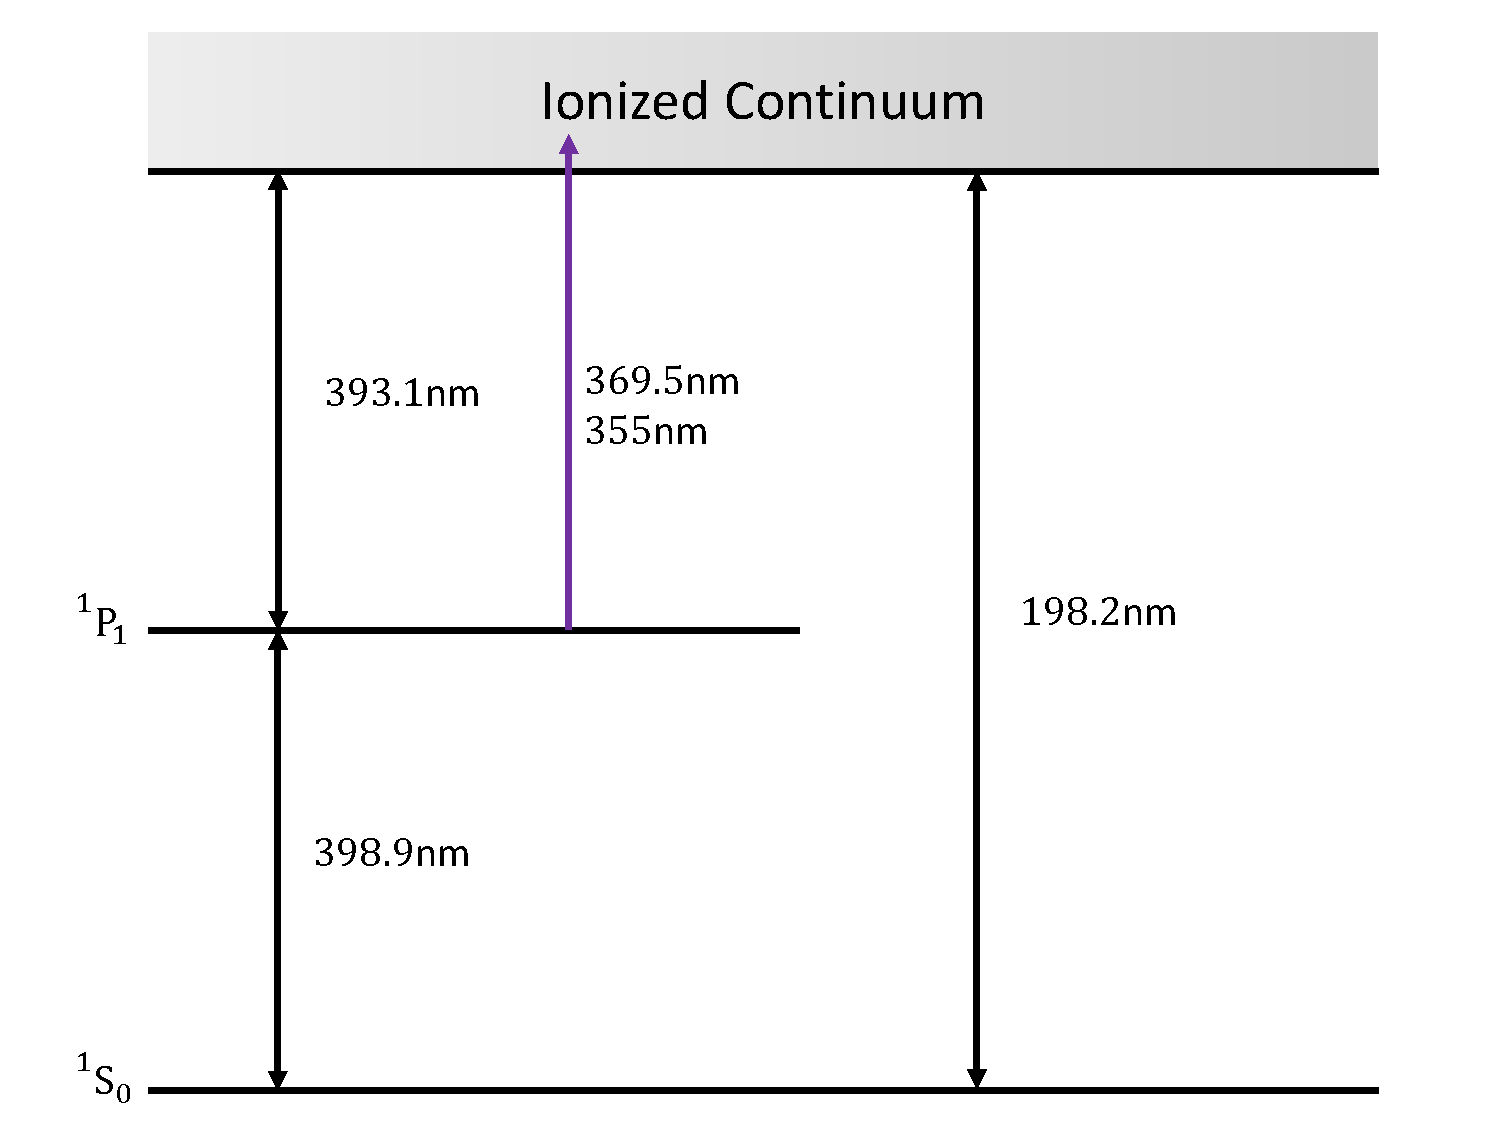
\includegraphics[width=0.5\linewidth]{fig_2_photo_ionization.pdf}
    \caption{Two-photon ionization scheme on ${ }^{171} \mathrm{Yb}^{+}$.}
    \label{fig:photo_ionization}
\end{figure}

Two-photon ionization allows for more precise control of isotope choice. The desired atomic source is often enriched, with an abundance as high as 91.7\%, the remainder consists of various natural isotopes, such as ${ }^{174} \mathrm{Yb}$, ${ }^{172} \mathrm{Yb}$, ${ }^{168} \mathrm{Yb}$ etc. Assume 50 ions in a large-scale trapped-ion quantum computer, and the average number of dark isotopes is 4. Thankfully, the intermediate level 398.91 nm transition exhibits an isotope-shift, which may be used to differentiate between isotopes. Doppler shift is a practical consideration that requires further care. The 398.91 nm laser is oriented perpendicular to the atomic flux to mitigate the Doppler effect. Isotope-selective loading of ions is possible in this setup, increasing the likelihood of the desired isotope, and this may be improved by decreasing the power of the 398.91 nm laser to achieve a narrow linewidth , although this might delay loading speed. Clock states, $\left|\downarrow_z\right\rangle \equiv\left|F=0, m_F=0\right\rangle$ and $\left|\uparrow_z\right\rangle \equiv\left|F=1, m_F=0\right\rangle$, encode the qubit. Doppler cooling, optical pumping and state detection all employ the cyclic transition between the $6^2 P_{1 / 2}$ states and the ground state $6^2 S_{1 / 2}$. A magnetic field applied externally causes a splitting of the $|F=1\rangle$ manifolds through the Zeeman effect at a rate of roughly 1.4 MHz/G, whereas the second-order Zeeman effect dominates the clock qubits at a rate of about 310 Hz/$\mathrm{G}^2$.

Routine ion loading procedures include directing an atomic beam to the loading zone, where several laser beams are utilized to photoionize the atoms. A needle and some shards of metal are all that make up the oven, enriched in 174Yb and 171Yb in separate ovens. On the outside, a current loop is created by connecting the needle's head and tail with Kapton wires to the positive and negative terminals of the power supply. No part of the needle should be anchored to the floor of the chamber. That's because doing so would generate a substantial current to flow into the ground. Since current flows preferentially toward a lower potential, this phenomena may be prevented by isolating the negative poles of the current source from the ground. Keep in mind that while powering the oven for the first time, we must increase the current gradually so as not to accidentally ignite it and safeguard the SAES pump. The first time you use an oven, numerous grimy items will likely be fired out, which might cause the SAES gauge current to rise to the order of A. The atoms are expelled into the trap's central zone after the oven is heated for several minutes.

\begin{figure}
    \centering
    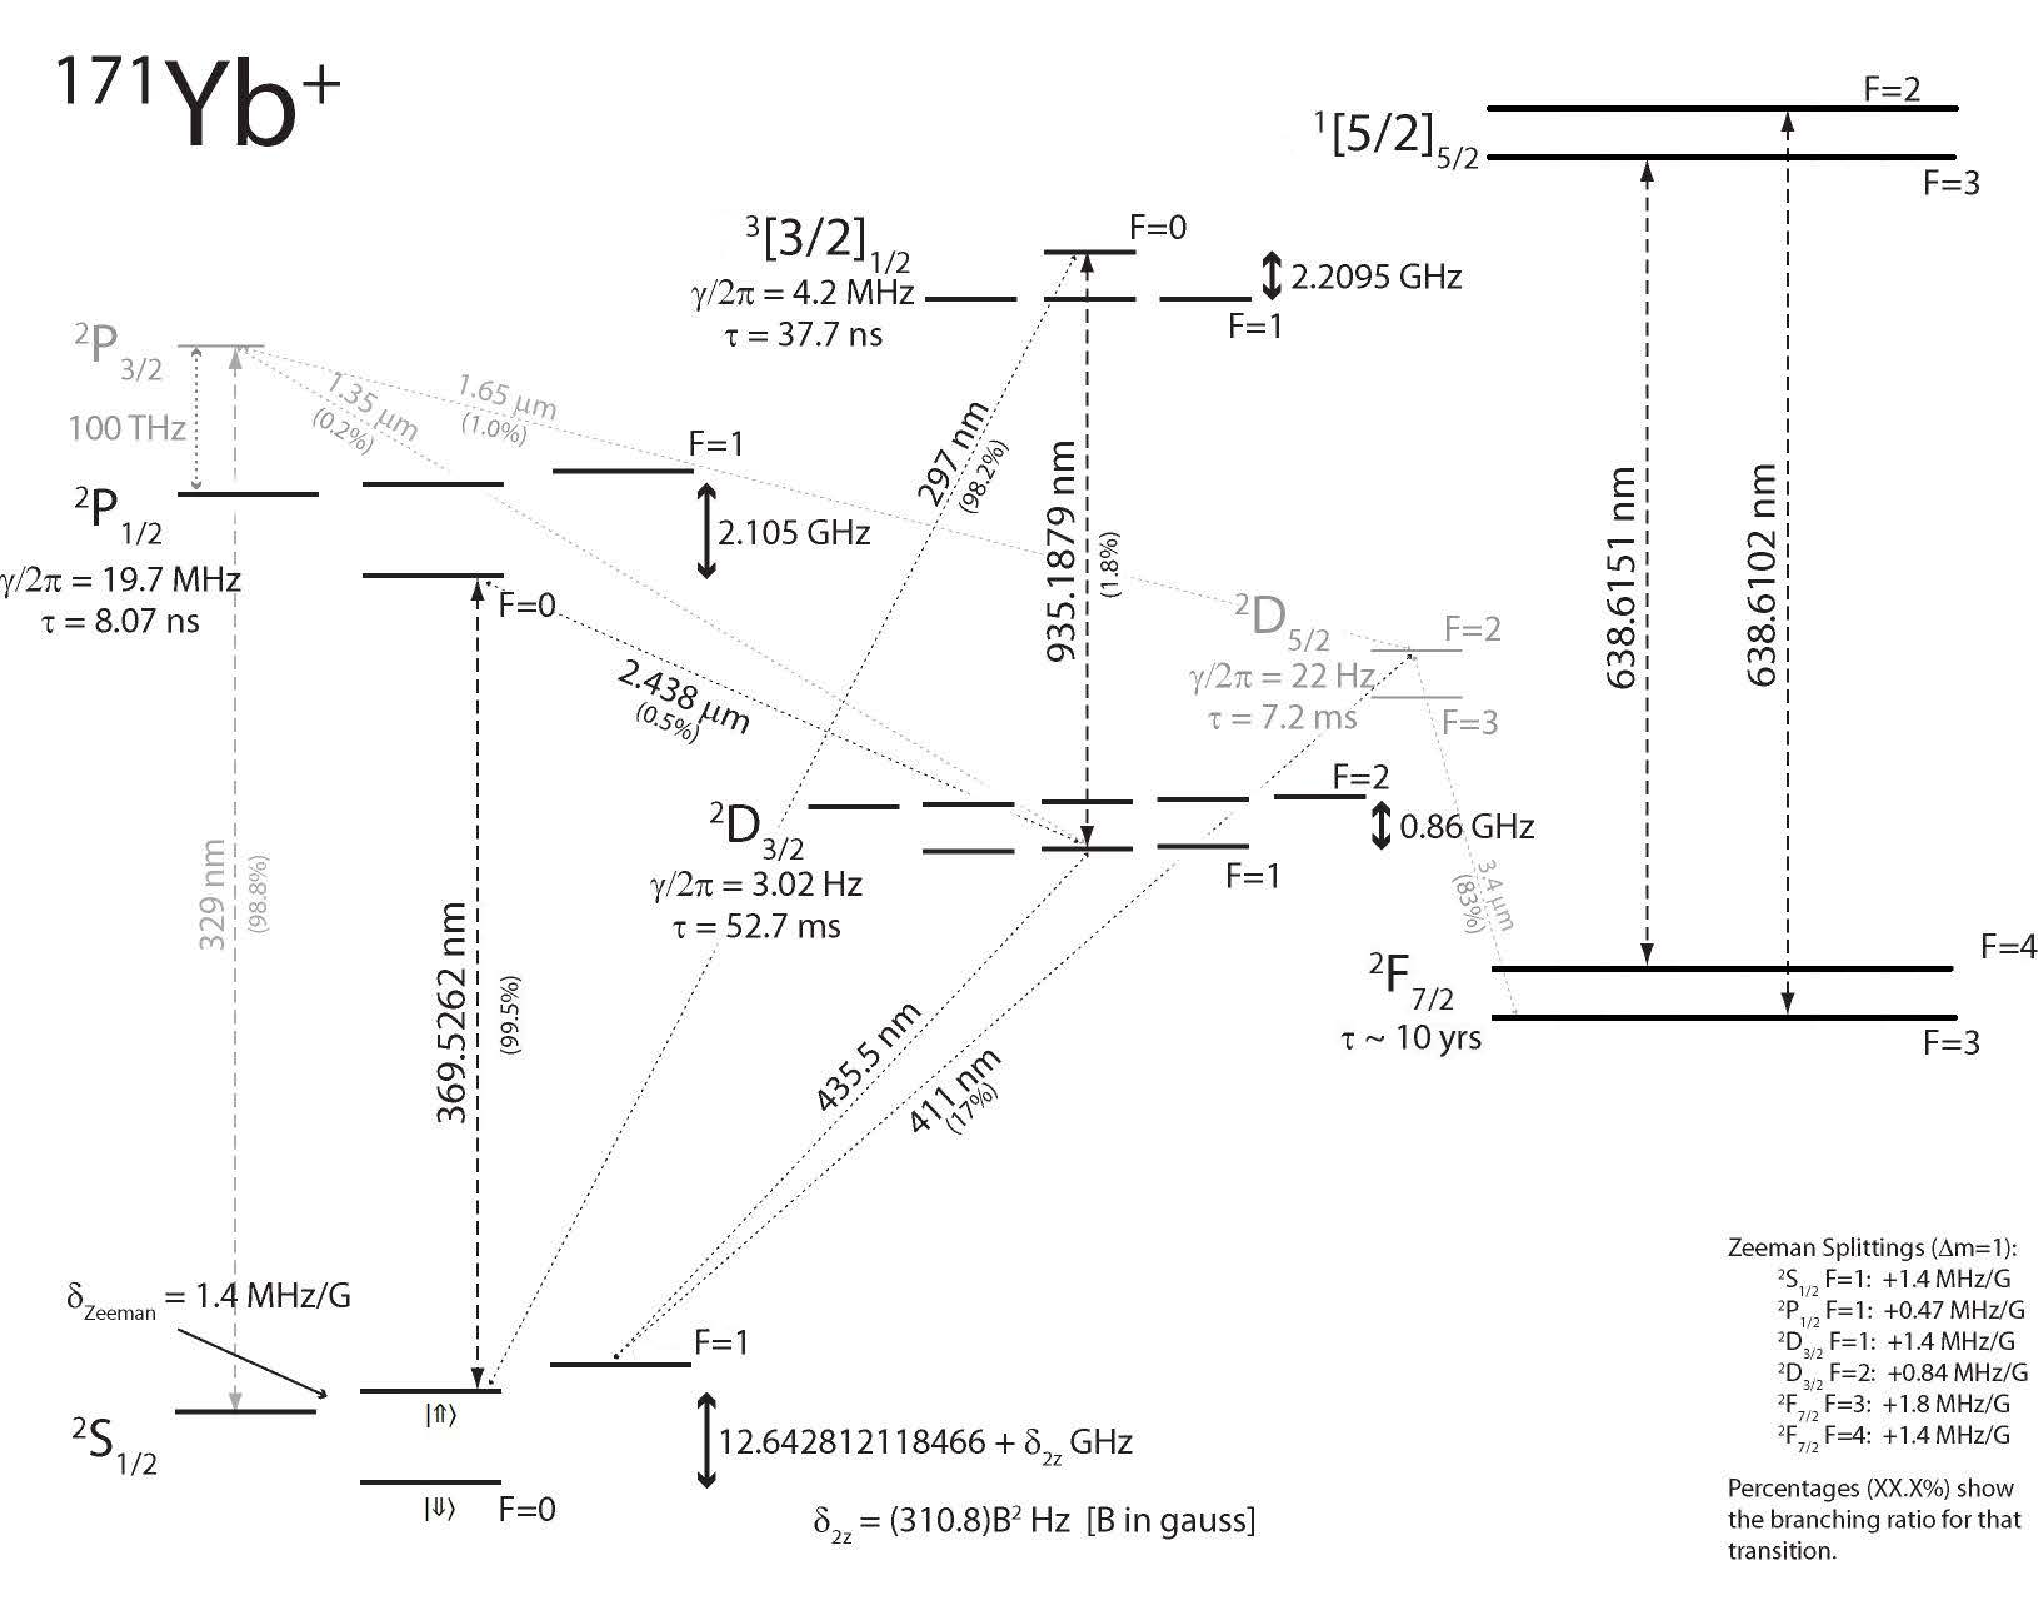
\includegraphics[width=1.0\linewidth]{fig_2_energy_level.pdf}
    \caption{${ }^{171} \mathrm{Yb}^{+}$ energy level diagram.}
    \label{fig:energy_level}
\end{figure}

\subsection{Doppler Cooling}

Ions have too wide of a motional area to be detected after they have been loaded into the trap since they are still very hot. We must first cool down the heated ions and produce the Coulomb crystal in order to stabilize and crystallize them. Doppler cooling is a method of rapidly cooling ions by utilizing a cyclic transition whose excited state has a very short lifetime and, therefore, a very high cooling rate. Doppler cooling is achieved in the ${ }^{171} \mathrm{Yb}^{+}$ system using a red-detuned laser to access $6^2 P_{1 / 2}$ levels with a lifetime of around 8.12 ns, a natural linewidth of 19.6 MHz, and a transition of 369.5263 nm.

Doppler cooling of ions is shown in a simplified model, where ion micromotion is disregarded and the trapping potential is represented by the time-independent pseudo harmonic potential $V(z)=\frac{1}{2} m \omega_z^2 z^2$ just in the z direction. Although the trapped ion's motion is no longer in the quantum domain after Doppler cooling, it can be treated as a classical motion with a velocity that obeys $v(t)=v_0 \cos \left(\omega_z t\right)$. Let us consider the hypothetical case of a single, moving laser interacting with a trapped two-level ion consisting only of S and P states. One cycle of absorption and spontaneous emission occurs in a time period where the ion's velocity does not vary noticeably if the radiative decay rateof the P-level is significantly bigger than the motional frequency. In this scenario, we may represent the average radiation pressure exerted on an ion as a continuous force that varies with its speed. A photon's absorption causes an ion's momentum to increase by $\Delta \mathbf{p}=\hbar \mathbf{k}$ in the direction of the photon's wave vector, and the ion's subsequent spontaneous emission likewise increases its momentum. After many cycles of absorption and emission, the ion will be slowed when the wave vector contains a component along the direction of motion, but the direction of the momentum kick due to spontaneous emission is random across cycles.

The Doppler cooling limit $T_{\min }=\hbar \Gamma(1+\chi) /\left(4 k_B\right)$ can be achieved by laser detuning $\Delta=-\frac{\Gamma}{2}$, where $\chi$ is the geometrical factor for spontaneous emission, $\Gamma=\sqrt{1+s} \Gamma_0$ is the effective linewidth broadened by power, $s$ is the saturation parameter and the saturation intensity is $I_{\text {sat }}=\frac{\pi h c \Gamma_0}{3 \lambda^3}=510 \mathrm{~W} / \mathrm{m}^2$. In addition, re-pumping $|\downarrow\rangle$ back to the cycled transition necessitates an additional frequency component with a detuning of 14.748 GHz. Moreover, the influence of the hyperfine levels must be taken into account, therefore a laser with a wavelength of 935.1880 nm and a sideband of 3.0695 GHz are needed. The branch ratio from level $6^2 P_{1 / 2}$ to level $5^2 D_{3 / 2}$ is non-zero at 0.5\%. Doppler cooling may be employed to achieve a final state with a phonon number below 10, where the crystal is stable against certain heating influences from the environment.

\begin{figure}
    \centering
    \subcaptionbox{Doppler cooling.}
    {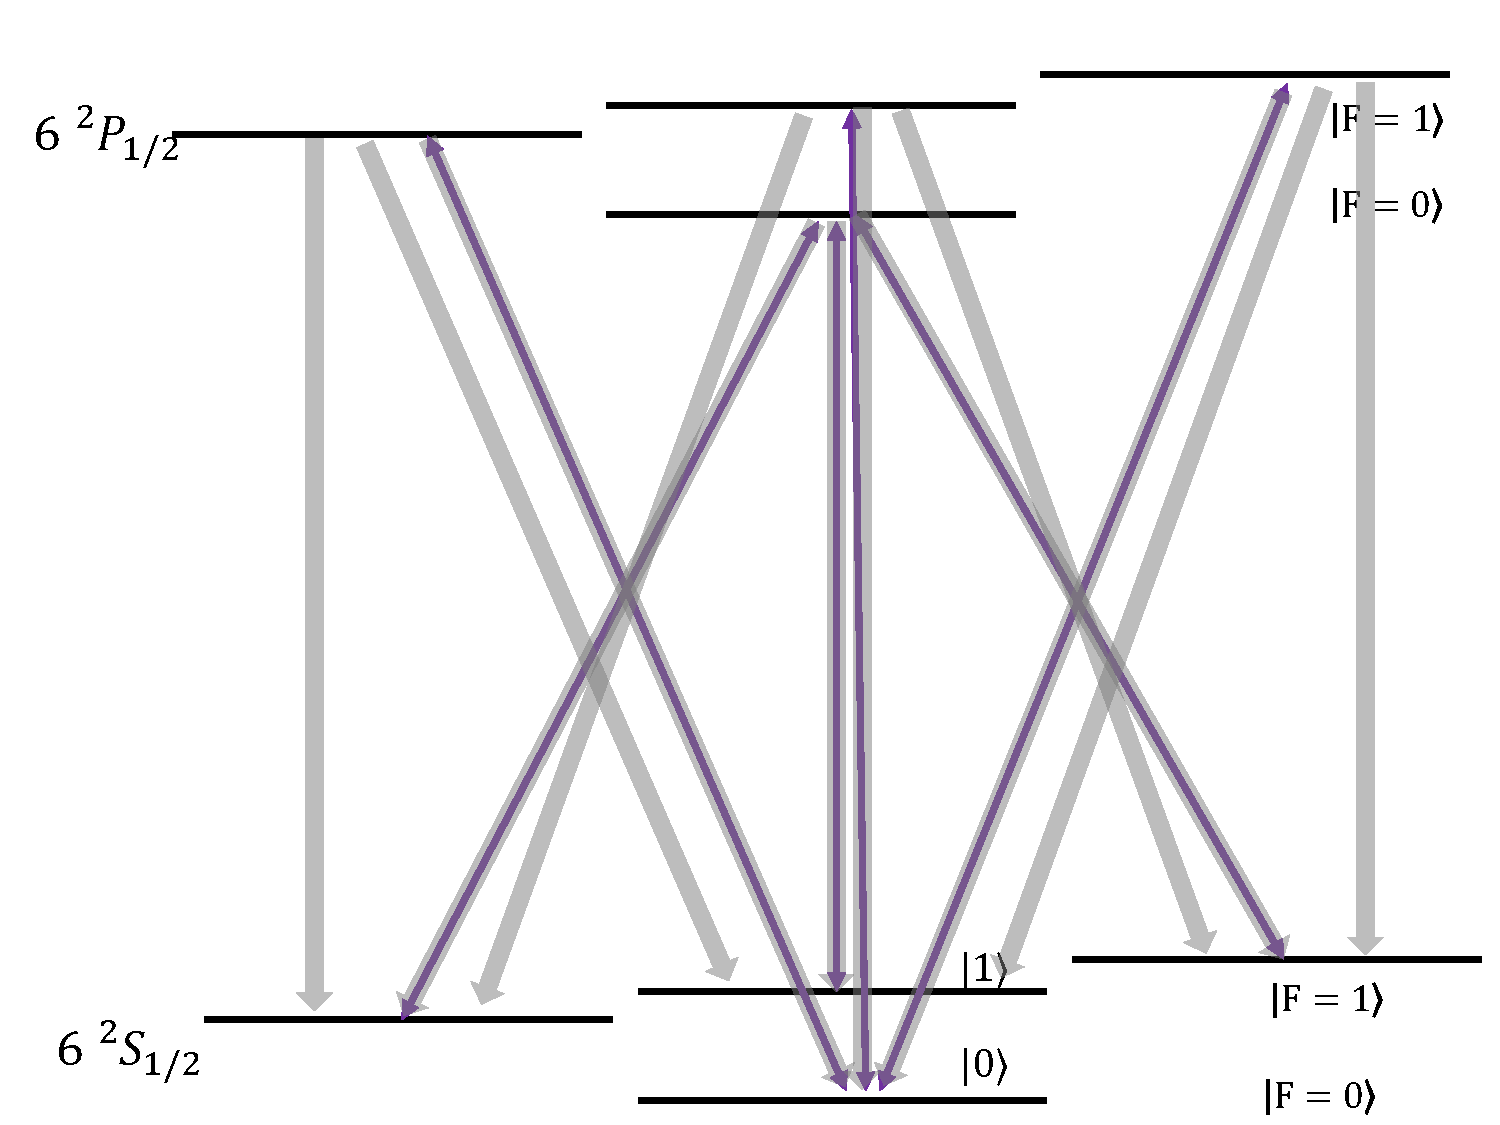
\includegraphics[width=0.4\linewidth]{fig_2_370_transitions_cooling.pdf}}
    \subcaptionbox{Optical pumping.}
    {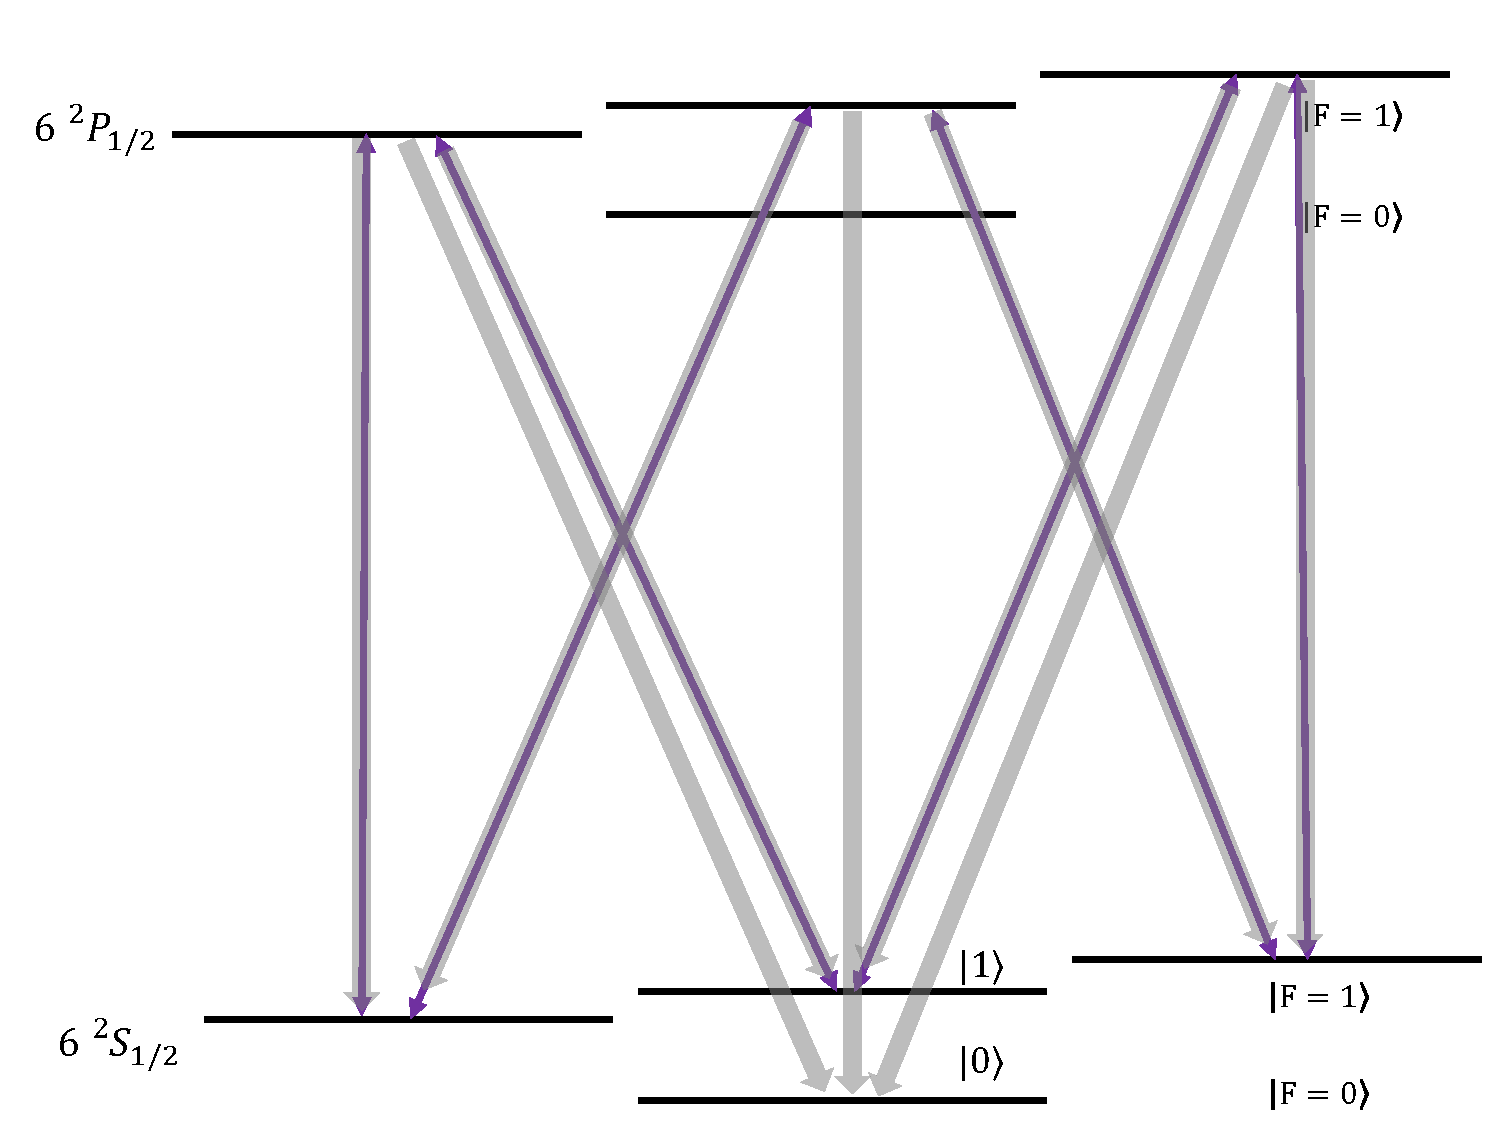
\includegraphics[width=0.4\linewidth]{fig_2_370_transitions_pumping.pdf}}
    \subcaptionbox{State detection.}
    {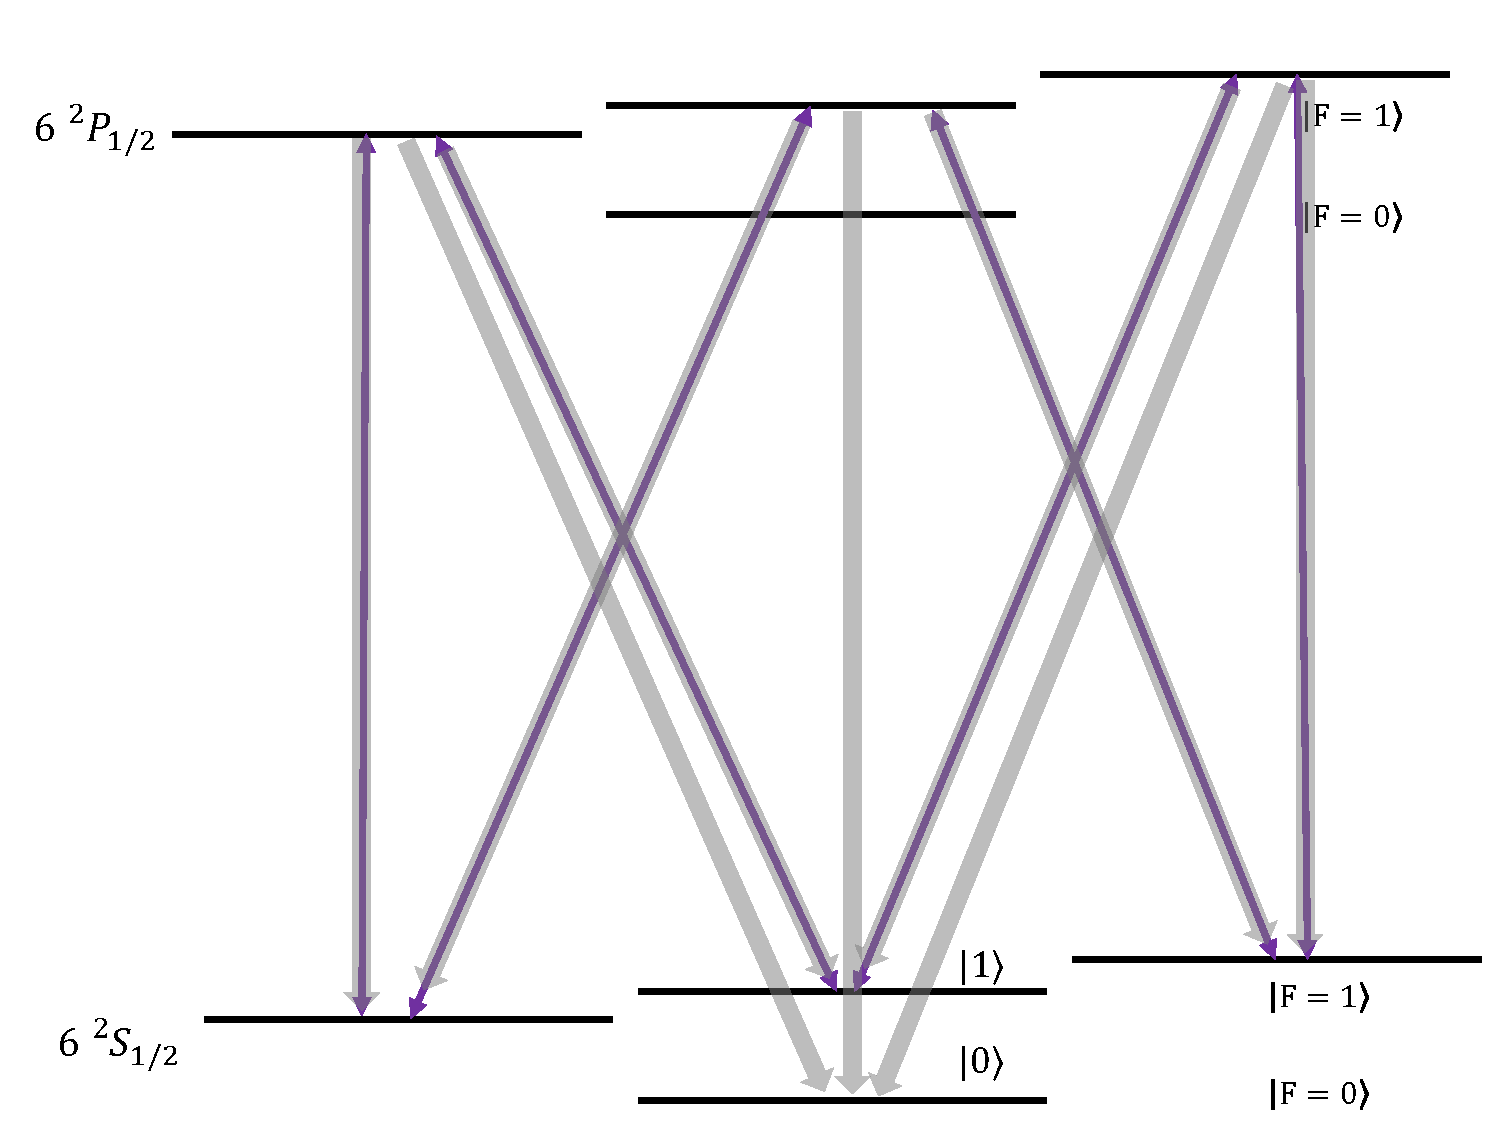
\includegraphics[width=0.4\linewidth]{fig_2_370_transitions_pumping.pdf}}
    \caption{The relevant transitions for 369.52 nm laser}
    \label{fig:370_transitions}
\end{figure}

\subsection{Optical Pumping}

When the ions have been cooled, the $\left|\downarrow_z\right\rangle$ state is prepared using optical pumping. Laser at 370 nm is stimulated when the ${ }^2 \mathrm{~S}_{1 / 2} \mathrm{~F}=1$ to ${ }^2 \mathrm{P}_{1 / 2} \mathrm{~F}=1$ transition occurs. If the ion enters the ${ }^2 \mathrm{P}_{1 / 2} \mathrm{~F}=1$ manifold, it may spontaneously decay to any of the ${ }^2 \mathrm{~S}_{1 / 2}$ states. The ion is $\sim$ 10GHz off resonant from the nearest transition. From the ${ }^2 \mathrm{P}_{1 / 2} \mathrm{~F}=1$ state, the ion has a 1/3 chance of decaying to the $\left|\downarrow_z\right\rangle$ state. According to the energy diagram, the optical pumping beam has to include both linear and circular components of polarization.

\subsection{State Detection}

An experiment's initial step is always preparing the $\left|\downarrow_z\right\rangle$ ion chain. The next step is to actually do the experiment, followed by analysis. When the $\hat{\sigma}_z$ operator is used for measurements, the $\left|\uparrow\right\rangle$ and $\left|\downarrow_z\right\rangle$ states of the ions are the only viable results.

It is possible to determine the state of the ion by shining light with a wavelength of 370 nm onto an ion chain that is resonant with the ${ }^2 \mathrm{~S}_{1 / 2} \mathrm{~F}=1$ to ${ }^2 \mathrm{P}_{1 / 2} \mathrm{~F}=0$ transition. This kind of light is known as a detecting light. The detecting light will only resonate with the $\left|\uparrow\right\rangle$ state if it is present. It is possible for the ion to decay spontaneously to any of the ${ }^2 \mathrm{~S}_{1 / 2} \mathrm{~F}=1$ levels. Since it is desirable to have numerous absorption or emission events, the beam has all possible polarization components. This allows the detection process to continue without interruption until sufficient photons have been gathered to determine the ion state. The ion fluoresces isotropically when exposed to the detecting light, and a portion of the light that is emitted by it is gathered by imaging optics and directed onto an EMCCD camera in order to read out the spin state. The detection light has a minuscule chance of off-resonantly exciting either spin state to the ${ }^2 \mathrm{P}_{1 / 2} \mathrm{~F}=1$ manifold, where the ion may subsequently decay into the other spin state and induce detection errors. This happens because of the ${ }^2 \mathrm{P}_{1 / 2} \mathrm{~F}=1$ manifold.

Doppler cooling, optical pumping, and state detection are all examples of operations that entail spontaneous decay to the ${ }^2 \mathrm{~S}_{1 / 2} \mathrm{~F}=1$ manifold of states. Hence, if the Zeeman states are degenerate, the mechanism of coherent population trapping may be used to pump the ion into a dark state. As a result, an application of a B-field is made to the ions in order to disrupt this degeneracy and stop the trapping of coherent populations. In the location where the ions are located, the B-field strength is XX G, and the Zeeman splitting from the $\left|\uparrow\right\rangle$ state is measured XX MHz.

We are able to determine the state of the spins in the ion chain by capturing the spin-dependent fluorescence using a site-resolving image Andor IXon Ultra 888 EMCCD camera. During the state detection process, a resonant laser with a wavelength of 370 nm is shone between $\left|\uparrow\right\rangle$ and $\left|\downarrow_z\right\rangle$. When the qubit is in the $\left|\downarrow_z\right\rangle$ state, a small amount of photons are scattered off, however when the spin state is in the $\left|\uparrow\right\rangle$ state, a significant number of photons are scattered off. The binary threshold for spin-state discrimination is determined by calibrating the number of photons dispersed from the bright $\left|\uparrow\right\rangle$ state and the dark $\left|\downarrow_z\right\rangle$ state of each spin at the beginning of the process of collecting data on those spins. The bright and dark states of the setup used in this thesis have an average fidelity of more than 97 \%, which is suitable for the quantum memory experiments. The off-resonant mixing of spin states during detection, crosstalk between nearby ions, noise from the electronic camera, and noise from the laser are the primary causes of mistake in this case.


\section{The Linear Paul Trap}

According to one of Maxwell's equations, $\nabla \cdot \vec{E}=0$, the electric field will not diverge in a region where there is no free charge density. This conclusion may be drawn from the fact that: Earnshaw deduced from this equation that it was mathematically impossible for a charged particle to be connected in a static electric field in all directions at the same time. Yet, in order to condense charged particles, either oscillating electric fields or a combination of static electric and magnetic fields are required. In this experiment, the RF trap is the primary focus.

Assuming for the sake of this discussion that the ions have a positive charge, mathematically express the criteria of an accessible potential that requires minima in any direction as shown below.

\begin{equation}\label{eq:minima}
    \frac{\partial \mathbf{E}}{\partial x_i}=-\frac{\partial^2 \Psi}{\partial x_i^2}<0, x_i \in\{x, y, z\}
\end{equation}

However, Eq.~\eqref{eq:minima} contradicts of the Laplacian equation for static electric fields in vacuum, which states that else there would never be a global minimum in any of the directions otherwise $\frac{\partial \mathbf{E}}{\partial x_i}=0$

\begin{equation}
    \nabla^2 \Psi=0
\end{equation}


The ion trap technique, which uses a mix of DC and RF oscillating electric fields, offers a fortunate alternative to the traditional method of confining ions in a vacuum environment. It is possible to write down the broad potential of a Paul trap as

\begin{equation}\label{eq:rfpotential}
    \Psi(x, y, z)=\frac{U}{2}\left(\alpha x^2+\beta y^2+\gamma z^2\right)+\frac{V}{2} \cos (\Omega t)\left(\alpha^{\prime} x^2+\beta^{\prime} y^2+\gamma^{\prime} z^2\right)
\end{equation}

$\alpha, \beta, \gamma, \alpha^{\prime}, \beta^{\prime}, \gamma^{\prime}$ are geometrical factors. A potential of this kind may be generated using hyperbolic electrodes, the geometrical factors involved are precisely $1 / r^2$, where $r$ denotes the distance to the electrodes. Unfortunately, the hyperbolic electrodes restrict the optical access. There are some novel designs for traps with high optical access, but the geometrical considerations need to take into account the approximations that are necessary since the hyperbolic electrodes are not ideal. There is an extra restriction for the geometrical factors that must be satisfied in order to satisfy the Laplacian equation

\begin{equation}
    \alpha+\beta+\gamma=0,\quad \alpha'+\beta'+\gamma'=0
\end{equation}

To be more specific, a Paul trap with the parameters $\gamma^{\prime}=0, \alpha=\beta=-\frac{\gamma}{2}, \alpha^{\prime}=-\beta^{\prime}$ is referred to as a linear trap. In a linear trap, charged particles are only confined by a static field in one direction, while RF fields are used to confine them in the other two directions.

\subsection{Mathieu Equation}

With a Paul trap, it is possible to decouple the motion of charged particles in three different directions. In this case, we will treat in $x$ for the sake of simplicity following,

\begin{equation}\label{eq:motion}
    m \frac{\mathrm{d}^2 x}{\mathrm{~d} t^2}=-Q\left(\alpha U x+\alpha^{\prime} V \cos (\Omega t) x\right)
\end{equation}
substitute $\tau=\frac{\Omega t}{2}, a_x=\frac{4 Q U \alpha}{m \Omega^2}, q_x=\frac{2 Q V \alpha^{\prime}}{m \Omega^2}$, Eq.~\eqref{eq:motion} can be simplified as a Mathieu equation

\begin{equation}
    \frac{\mathrm{d}^2 x}{\mathrm{~d} \tau^2}+\left(a_x x-2 q_x \cos (2 \tau) x\right)=0
\end{equation}

In this case, the solution of the lowest order is shown together with the assumptions that $\left|a_x\right|, q_x^2 \ll 1$,

\begin{equation}
    \beta_x=\sqrt{a_x+\frac{q_x^2}{2}}, \quad x(t)=2 A C_0 \cos \left(\beta_x \frac{\Omega t}{2}\right)\left[1-\frac{q_x}{2} \cos (\Omega t)\right]
\end{equation}

This is a bounded solution with periodic frequency $\omega_x=\frac{\beta_x \Omega}{2}$, which is often referred to as secular motion. The second component in frequency $\Omega \pm \omega_x$ represents the intrinsic micromotion that is induced by the RF fields.

In a further approximation, it is possible to construct an effective time-independent potential to describe the dynamics of charged particles in an RF Paul trap. An example in $x$ is presented below, and we assume that the charge is equal to $e$.

\begin{equation}
    E(x, t)=E_0(x) \cos (\Omega t)
\end{equation}

\begin{equation}
    F(x, t)=m \ddot{x}=e E_0(x) \cos (\Omega t)
\end{equation}

where $E_0(x)$ is independent of the time-varying potential and solely depends on positional information. Imagine a crystal that has been stabilized such that all of its ions remain in close proximity to their positions of equilibrium. The only new vibrations that occur are those that are caused by the RF fields.

\begin{equation}\label{eq:staticmotion}
    x=x_0-\frac{eE_0(x_0)}{m\Omega^2}\cos(\Omega t)
\end{equation}

This is the first-order solution to the motion, and we may do additional Taylor expansion at the equilibrium location $x_0$ to the electric field as well, although this is not necessary.

\begin{equation}
    \begin{aligned}
        E_0(x) & =E_0\left(x_0\right)+\left.\frac{\partial E_0(x)}{\partial x}\right|_{x_0}\left(x-x_0\right)                                                    \\
               & =E_0\left(x_0\right)-\left.\frac{\partial E_0(x)}{\partial x}\right|_{x_0}\left(\frac{e E_0\left(x_0\right)}{m \Omega^2} \cos (\Omega t)\right) \\
               & =E_0\left(x_0\right)-\left.\frac{e}{2 m \Omega^2} \frac{\partial E_0^2(x)}{\partial x}\right|_{x_0} \cos (\Omega t)
    \end{aligned}
\end{equation}

\begin{equation}
    \begin{aligned}
        F(x, t)=m \ddot{x} & =e E_0\left(x_0\right) \cos (\Omega t)-\left.\frac{e^2}{2 m \Omega^2} \frac{\partial E_0^2(x)}{\partial x}\right|_{x_0} \cos ^2(\Omega t)        \\
                           & =e E_0\left(x_0\right) \cos (\Omega t)-\left.\frac{e^2}{2 m \Omega^2} \frac{\partial E_0^2(x)}{\partial x}\right|_{x_0}(1+\cos (2 \Omega t)) / 2
    \end{aligned}
\end{equation}

Assess the influence on average, excluding out the variables that are rapidly fluctuating,

\begin{equation}
    \bar{F}(x)=-\left.\frac{e^2}{4 m \Omega^2} \frac{\partial E_0^2(x)}{\partial x}\right|_{x_0}
\end{equation}

where \(E_0(x)=-\alpha'V x\) for the general potential, it is a harmonic confinement that does not rely on whether the ions are positively or negatively charged, and it controls the secular motion of ions inside the trap. Additional words include the source of micromotion, which has an oscillation that is much more rapid and is defined by frequency \(\Omega\). Hence, one way to define the pseudo potential is as follows,

\begin{equation}\label{eq:pseudo_potential}
    \Psi_{ps}=\frac{e}{4m\Omega^2}E_0^2(x)=\frac{e\alpha'^2V^2}{4m\Omega^2}x^2
\end{equation}

This re-creates the conclusion that Earnshaw's theorem came to. It is a valid approximation for equilibrium positions and secular motion of charged particles in an RF trap, and it can be used to calculate the principal axes taking both DC and RF fields into account. The secular frequency is \(\omega_x=\frac{e\alpha' V}{\sqrt{2}m\Omega}\), which is consistent with the Mathieu equation. The static confinement can also be taken into account, which is also a harmonic term.

\subsection{Normal Modes}

Since the normal modes are entirely decoupled from all directions, particularly the transverse modes that we are working on, we employ a chain of trapped ${ }^{171} \mathrm{Yb}^{+}$ ions as the quantum memory in a linear Paul trap. This allows us to study the transverse modes. It is necessary for the trap frequencies to adhere to the relation Eq.~\eqref{eq:linear_chain} if the Coulomb crystal is to be contained inside a linear chain.

\begin{equation}\label{eq:linear_chain}
    \left(\frac{\omega_r}{\omega_z}\right)^2 \geq \frac{N^{1.73}}{2.53}
\end{equation}

where \(N\) is the number of ions, \(\omega_r\) refers to either the transverse mode \(\omega_x\) or \(\omega_y\), and \(\omega_z\) refers to the axial mode with DC confinement.

Instead of using the straightforward Mathieu equation, one needs take into consideration the Coulomb interaction that occurs between the ions when there are a greater number of ions fed into the trap. Both the externally imposed pseudo potential and the Coulomb interactions that occur between the ions work together to decide the shape of the ion crystal.

The inter-ion spacings would not be uniform under a harmonic potential similar to Eq.~\eqref{eq:rfpotential}, where spacings at the center of an ion chain would be much more tight but loose at the edge. This would require much higher RF potential or lower DC potential to satisfy Eq.~\eqref{eq:linear_chain}, or else there would be an unstable transition to zigzag mode. Here, we consider \(N\) ions in In order to solve the issue, quartic potential is required. This is because increasing the number of electrodes along the z-axis will bring the inter-ion spacings closer to being uniform. As the micromotion is negligible in comparison to the secular motion and all of the ions are aligned with the RF null in the required configuration, the property of the ion crystal may be obtained using the pseudo potential while ignoring the time-dependent RF potential.

The potential in its broadest sense may be expressed as

\begin{equation}
    U=\sum_i\left(\frac{\alpha}{2} z_i^2+\frac{\beta}{4} z_i^4\right)+\sum_{i<j} \frac{e^2}{4 \pi \epsilon_0\left|z_i-z_j\right|}
\end{equation}

Here, we will define the length unit known as \(l=\qty(e^2/4\pi\epsilon_0\alpha)^{1/3}\), and after that, we will be able to rewrite the potential \(u_i\equiv z_i/l\) using dimensionless coordinates and dimensionless energy \(U'\equiv 4\pi \epsilon_0 lU/e^2\), respectively.

\begin{equation}\label{eq:dimensionlessaxialpotential}
    U'=\sum_i\qty(\frac{1}{2}u_i^2+\frac{\beta l^2}{4\alpha}u_i^4)+\sum_{i\ne j}\frac{sgn(\alpha)}{2\abs{u_i-u_j}}
\end{equation}\

where \(sgn(x)\) is the sign function.

% Once we have determined the ion number and the potential configuration \(\frac{\beta l^2}{\alpha}\), we can minimize the energy to find the equilibrium positions. Alternatively, we can solve the equations of gradient at equilibrium
% \begin{equation}\label{eq:gradient}
%     0=\pdv{U'}{u_i}=u_i+\frac{\beta l^2}{\alpha}u_i^3-sgn(\alpha)\sum_{i\ne j}\frac{u_i-u_j}{\abs{u_i-u_j}^3}
% \end{equation}

% Rather than perform the optimization with multiple variables, we can further reduce the problem to find the solutions of the gradient equations, which can be easily accomplished by some built-in functions of Wolfram Mathematica such as FindRoot or NSolve.

% After obtaining the equilibrium positions, the axial motional modes can be computed by the Hessian matrix
% \begin{equation}\label{eq:axial_hessian}
%     \pdv{U'}{u_i}{u_j}=\begin{cases}
%         1+\frac{3\beta l^2}{\alpha}u_i^2+\sum_{k\ne i}\frac{2sgn(\alpha)}{\abs{u_i-u_k}^3}, & i=j    \\
%         -\frac{2sgn(\alpha)}{\abs{u_i-u_j}^3},                                              & i\ne j
%     \end{cases}
% \end{equation}

% To show a brief picture of the potential, we will give an example based on our BEM simulation of \(5\)-segment blade trap(See Sec.~\ref{sec:idealpotential}). For a harmonic potential \(\alpha> 0\), we can set the voltage of DC segments as \(\qty(1,\,0,\,0,\,0,\,1)\,\unit{V}\), the simulated results of \(60\) \yb{171} ions are shown in Fig.~\ref{fig:harmonic}, the length of the ion chain is about \(200\,\unit{\um}\), the lowest center-of-mass(COM) mode is \(92.76\,\unit{\kHz}\) and the potential depth by \(\pm 150\,\unit{\um}\) is about \(0.0065\,\unit{eV}\), and the inter-ion spacings are increasing from the center to the edge with a relative standard deviation(RSD) \(28.4\%\). For such a configuration, the repulsion among the central ions would be strongest and thus the zigzag transition would first take place in the center, which could be avoided by lowering the axial confinement or increasing the RF confinement.

% \begin{figure}[hbtp]
%     \centering
%     \subcaptionbox{}[0.5\linewidth]{\includegraphics[width=\linewidth]{harmonic_potential.pdf}}\hfill
%     \subcaptionbox{}[0.5\linewidth]{\includegraphics[width=\linewidth]{harmonic_spacing.pdf}}
%     \caption[Equilibrium positions and ion spacings in the harmonic potential]{\label{fig:harmonic}(a) The equilibrium positions, (b) The inter-ion spacings of \(60\) \yb{171} ions in the harmonic potential, the relative standard deviation(RSD) is \(28.4\%\).}
% \end{figure}

% However, we have two degrees of freedom for the axial confinement so that we can engineer a quartic potential \(\alpha<0,\,\beta>0\), the voltages can be set \(\mqty(10&0&2.4&0&10)\,\unit{V}\) to achieve the same size of \(60\)-ion crystal in length of \(200\,\unit{\um}\), typically the COM mode frequency would be higher than the harmonic one and here it is \(95.57\,\unit{\kHz}\). The potential depth by \(\pm 150\,\unit{\um}\) is about \(0.0125\,\unit{\eV}\) and the inter-ion spacings are much more uniform with RSD \(11.9\%\), which can be further improved if we have more DC electrodes. In addition, the bandwidth of the normal modes can be narrower for quartic potential, as seen in Fig.~\ref{fig:narrow_bandwidth}, this would enable us a better control over the normal modes such as the ground state cooling. The corresponding \(60\) dimensionless normal mode vectors are depicted as in Fig.~\ref{fig:axial_modes}, the mode structure is completely different that modes are distributed more uniformly for quartic potential and the strengths of normal mode vectors represent the contribution for specific normal modes.
% \begin{figure}[hbtp]
%     \centering
%     \subcaptionbox{}[0.5\linewidth]{\includegraphics[width=\linewidth]{quartic_potential.pdf}}\hfill
%     \subcaptionbox{}[0.5\linewidth]{\includegraphics[width=\linewidth]{quartic_spacing.pdf}}
%     \caption[Equilibrium positions and ion spacings in the quartic potential]{\label{fig:quartic}(a) The equilibrium positions, (b) The inter-ion spacings of \(60\) \yb{171} ions in the quartic potential, the relative standard deviation(RSD) is \(12.0\%\)}
% \end{figure}

% \begin{figure}[hbtp]
%     \centering
%     \subcaptionbox{Harmonic potential.}[0.5\linewidth]{\includegraphics[width=\linewidth]{harmonic_freq.pdf}}\hfill
%     \subcaptionbox{Quartic potential.}[0.5\linewidth]{\includegraphics[width=\linewidth]{quartic_freq.pdf}}
%     \caption[The axial normal mode frequencies]{\label{fig:narrow_bandwidth}The axial normal mode frequencies of \(60\) \yb{171} ions in two kinds of potential form.}
% \end{figure}

% \begin{figure}[hbtp]
%     \centering
%     \subcaptionbox{Harmonic potential.}[0.5\linewidth]{\includegraphics[width=\linewidth]{harmonic_axial_mode.pdf}}\hfill
%     \subcaptionbox{Quartic potential.}[0.5\linewidth]{\includegraphics[width=\linewidth]{quartic_axial_mode.pdf}}
%     \caption[The axial normal mode vectors]{\label{fig:axial_modes}The dimensionless normal mode vectors along trap axis of \(60\) \yb{171} ions in two kinds of potential form, the mode index starts from the lowest COM mode and the strengths of mode vectors represent the contribution to specific modes.}
% \end{figure}

% As for the transverse modes, things would be different. The COM mode is the highest one and the bandwidth is near the axial COM mode\cite{zhu2006trapped}, thus the transverse modes are much more crowded. We can further include the transverse terms in a general form
% \begin{equation}\label{eq:allpotential}
%     U=\sum_i\qty(\frac{\alpha}{2}z_i^2+\frac{\beta}{4}z_i^4+\frac{1}{2}m\omega_x^2x_i^2+\frac{1}{2}m\omega_y^2y_i^2)+\sum_{i<j}\frac{e^2}{4\pi\epsilon_0\abs{\vb{r_i}-\vb{r_j}}}
% \end{equation}

% For a linear chain configuration, the equilibrium positions for transverse \(x,\, y\) are quite clear that \(x_0=0,\,y_0=0\), and we can use the same dimensionless unit \(l\) to simplify the potential expression using notation \(uz=z/l,\, ux=x/l,\, uy=y/l\),
% \begin{equation}\label{eq:dimensionlesspotential}
%     \begin{aligned}
%         U' & =\sum_i\qty(\frac{1}{2}uz_i^2+\frac{\beta l^2}{4\alpha}uz_i^4+\frac{m\omega_x^2}{2\alpha}ux_i^2+\frac{m\omega_y^2}{2\alpha}uy_i^2)+\sum_{i\ne j}\frac{sgn(\alpha)}{2\abs{\vb{u_i}-\vb{u_j}}} \\
%            & =U_0+\sum_i\qty(\frac{m\omega_x^2}{2\alpha}ux_i^2+\frac{m\omega_y^2}{2\alpha}uy_i^2)-sgn(\alpha)\sum_{i\ne j}\frac{\qty(ux_i-ux_j)^2+\qty(uy_i-uy_j)^2}{4\abs{uz_i-uz_j}^3}
%     \end{aligned}
% \end{equation}
% where \(U_0\) is the one only related to coordinates \(uz_i\)'s, and we can neglect them without loss of generality when considering the transverse modes. We can also obtain the Hessian matrix for \(x,\, y\), and the results for \(x\) is present below, and RHS of the potential has the same dependence on the sign of \(\alpha\), in practice, we can directly use the absolute value,

% \begin{equation}\label{eq:transverse_hessian}
%     \pdv{U'}{ux_i}{ux_j}=\begin{cases}
%         \frac{m\omega_x^2}{\abs{\alpha}}-\sum_{k\ne i}\frac{1}{\abs{uz_i-uz_k}^3}, & i=j    \\
%         \frac{1}{\abs{uz_i-uz_j}^3},                                               & i\ne j
%     \end{cases}
% \end{equation}

% Here, we show an example of the above crystal, and set the transverse trap frequency as \(2\pi \times 2.47\,\unit{\MHz}\), clearly the transverse mode bandwidth is narrower for the quartic potential as shown in Fig.~\ref{fig:transverse_freq}, once the zigzag mode frequency is low and then the transition probability to a 2D zigzag pattern would be high.  In particular, the mode vectors are in a way the inverse of the axial one, as we can see in Fig.~\ref{fig:axial_modes} and Fig.~\ref{fig:transverse_modes}.
% \begin{figure}[hbtp]
%     \centering
%     \subcaptionbox{Harmonic potential.}[0.5\linewidth]{\includegraphics[width=\linewidth]{transverse_harmonic_freq.pdf}}\hfill
%     \subcaptionbox{Quartic potential.}[0.5\linewidth]{\includegraphics[width=\linewidth]{transverse_quartic_freq.pdf}}
%     \caption[The transverse normal mode frequencies]{\label{fig:transverse_freq}The transverse normal mode frequencies of \(60\) \yb{171} ions in two kinds of potential form.}
% \end{figure}

% \begin{figure}[hbtp]
%     \centering
%     \subcaptionbox{Harmonic potential.}[0.5\linewidth]{\includegraphics[width=\linewidth]{transverse_harmonic_mode.pdf}}\hfill
%     \subcaptionbox{Quartic potential.}[0.5\linewidth]{\includegraphics[width=\linewidth]{transverse_quartic_mode.pdf}}
%     \caption[The transverse normal mode vectors]{\label{fig:transverse_modes}The dimensionless normal mode vectors along transverse axes of \(60\) \yb{171} ions in two kinds of potential form, the mode index starts from the lowest zigzag mode and the strengths of mode vectors represent the contribution to specific modes.}
% \end{figure}



\section{notation}

${ }^{171} \mathrm{Yb}^{+}$

$6^2 P_{1 / 2}$

$|\downarrow\rangle$

$\left|\downarrow_z\right\rangle$

$\left|\uparrow\right\rangle$


% !TeX root = ./PhDThesis.tex

\chapter{Experimental setup}

The rate of background gas collisions with the ion chain is one of the scaling challenges in an ion-trapped system. Such collisions may destroy the qubit's information and result in the loss of the whole chain. Thus, it is essential to construct an extreme high vacuum (XHV) environment to reduce pressure of the background gas in the vacuum system.



\section{The cryostat}

The cryostat is the key equipment of the cryogenic trapped ion system \cite{RN58,RN38,RN59,RN260}. We need to pay attention to some key technical indicators when choosing the model of the cryostat, designing the internal support structure and the assembly structure of the trap-related components \cite{RN93}. The most critical technical indicators are cooling capacity and vibration. Low temperature is the advantage of the cryogenic trap over the room-temperature trap. We can achieve low pressure by cryo-pumping to reduce the collision \cite{RN134} rate of trapped ions with residual background gas, thereby increasing the lifetime of trapped ions. The price of cryo-pumping is additional vibration, however, the vibration can be reduced to a degree that does not affect quantum gate fidelity. In experiments, we often use these two parameters to characterize the cooling capacity. One is the lowest temperature that the system can reach when the cryogenic trap is not temperature stabilized, and the other is the heating power at the sample mount when the temperature of the cryogenic trap is stabilized above the liquid helium temperature zone and the vibration caused by liquid helium is reduced to a certain range. Another key technical indicator of the cryostat is the long-term stability at the sample, including changes in displacement and background electric field. This will affect the calibration period of the ion trap experiment. Calibration that is too frequent indicates a lack of robustness in the experiment system \cite{RN84}.

There are several different types of cryostats on the market. One of these is the flow cryostat, which has lower cryocooler vibration noise but requires constant replenishment of cold liquid coolant, which is expensive and time-consuming \cite{RN283}. In contrast, the cryogenic trapped ion system in our lab uses a closed-loop Gifford-McMahon cryostat \cite{RN284,RN285,RN39,RN282,RN206}. This type of cryostat uses closed-cycle helium gas as operation material in cooling cycle and does not require constant refilling of the coolant. It is very convenient to use and cheap to maintain as it only needs external electric supply.
One of the advantages of this closed-loop cryostat is that it has a vibration isolation system (VIS). The vibrating cold finger is mechanically separated from the main vacuum by a helium-filled exchange gas region at a pressure 0.03 bar above atmospheric. The vibration isolation system is the only mechanical coupling between the cold head and the main vacuum apparatus which is mounted on an optical breadboard. In the vibration isolation system region, it is sealed with a helium-confined rubber bellows. The helium gas serves as the thermal link between the cold finger and the sample mount where the ion trap is mounted. Another advantage of this closed-cycle cryostat is that its structure is relatively simple, and we can increase cooling capacity and reduce vibration through optimized design, because it is difficult to optimize each parameter independently in a complex system \cite{RN120}.

\begin{table}
    \centering
    \caption{Refrigeration capacity (typical).}
    \begin{tabular}{p{0.2\linewidth}p{0.3\linewidth}p{0.3\linewidth}}
        \toprule
                     & RDK-408D2                 & RDK-415D2                 \\
        \midrule
        First stage  & 40 Watts @ 43 (50Hz)      & 35 Watts @ 50K (50Hz)     \\
                     & 50 Watts @ 43 (60Hz)      & 45 Watts @ 50K (60Hz)     \\
        Second stage & 1.0 Watt @ 4.2K (50/60Hz) & 1.5 Watt @ 4.2K (50/60Hz) \\
        \bottomrule
    \end{tabular}
    \label{tab:refrigeration_capacity}
\end{table}

The cryostat is model SHI-4XG-15-UHV, designed and manufactured by Janis Inc \cite{RN121}. In order to reduce vibration, we provide some design suggestions. The cryostat consists of a cold head, an exchange gas space and a vacuum chamber.
The cold head is powered by a helium compressor. The models of cold head and helium compressor are RDK-415D2 and F70-H produced by Sumitomo Corporation of Japan. The cold head features two stages with different refrigeration capacity: the 40 K stage has $\sim$ 35 W, and the 4 K stage has 1.5 W, as shown in Table~\ref{tab:refrigeration_capacity}. The cold head must be fixed near the vacuum chamber, but there are only three interfaces of the cold head: the power supply, the supply high-pressure helium tube and the return high-pressure helium tube. Therefore, we placed the helium compressor and water cooler in the grey room of the laboratory to further isolate the source of vibration noise. The single continuous running time of the cold head can exceed 10,000 hours, which is enough for us to carry out long-term experiments.

\begin{figure}
    \centering
    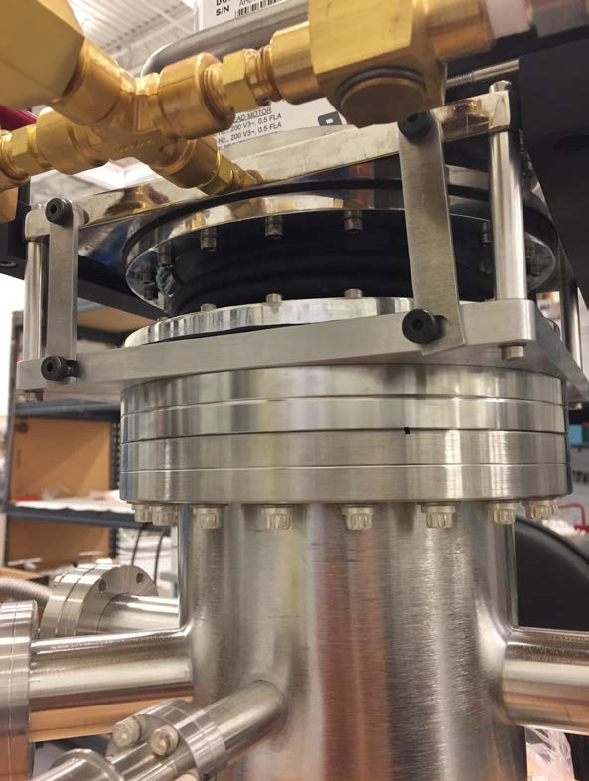
\includegraphics[width=0.5\linewidth]{fig_3_exchange_gas_space.pdf}
    \caption{Exchange gas space.}
    \label{fig:exchange_gas_space}
\end{figure}

The exchange gas space, as shown in Fig~\ref{fig:exchange_gas_space}, is mainly composed of rubber bellow, helium pressure gauge and some helium valves, the top and bottom are respectively connected to the cold head and the vacuum chamber. The role of bellow is to reduce the vibration generated by the cold head and directly transmitted to the vacuum chamber, because rubber is more elastic than stainless steel. I think it is worth trying to replace the rubber bellow with a stainless-steel sheet that has been bent many times, because using a rubber bellow may cause leakage in the long-term operation of the system. Leakage of rubber bellow may come from three aspects. Firstly, the rubber material will deteriorate after a long-time use, our system has a leakage problem after about 2 years of operation, which is manifested as water inside the exchange gas space after the process of cooling down and warming up. Secondly, the rubber bellow is prone to defects during machining, we contacted our supplier to process a new rubber bellow after we found the leakage problem, and found that some of the rubber bellow had defects on the surface during many attempts. Finally, the sealing method of rubber bellow is worse than that of stainless steel, our cryostat uses o-ring to seal rubber bellow \cite{RN133}. We tried to have the supplier process different rubber bellow to test the leakage, such as testing different materials and thickness of rubber bellow, in some poor cases after a single cooling and reheating process will appear leakage, we finally used silicone rubber bellow and the thickness is twice the original and no leakage has been found so far.



\section{Cryogenic and UHV system}

\begin{figure}
    \centering
    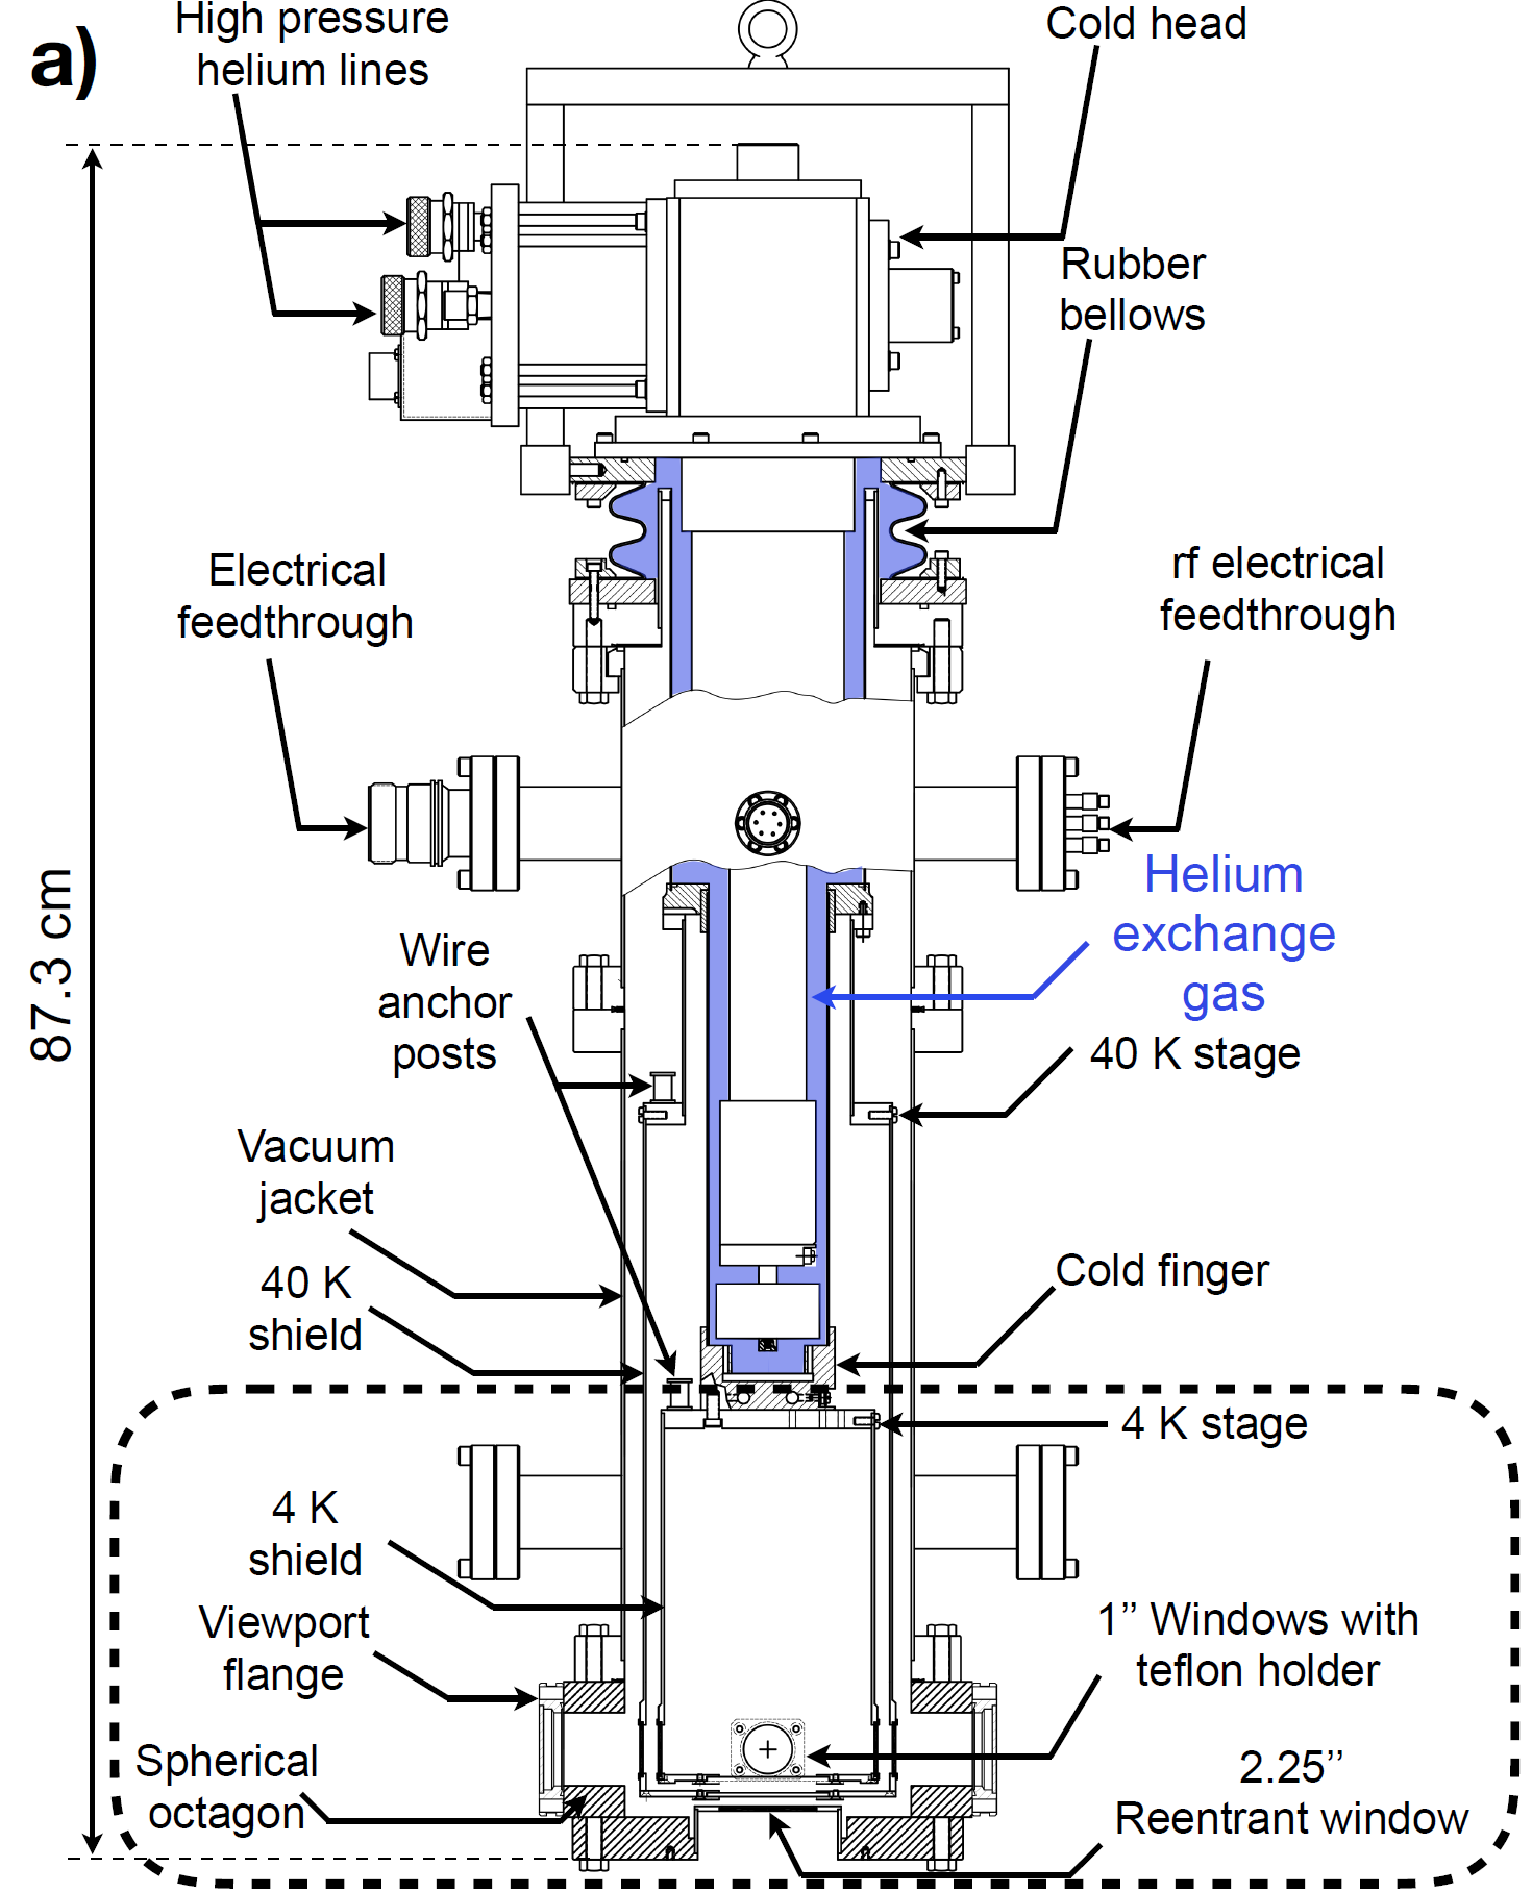
\includegraphics[width=0.7\linewidth]{fig_3_cryostat_a.pdf}
    \caption{The side section view of the Gilford-McMahon cryostat.}
    \label{fig:cryostat_a}
\end{figure}

The vacuum chamber resembles a cylinder with a diameter of about 200 mm and a height of about 600 mm. Externally, the upper part of the vacuum chamber has some feedthroughs connecting the electrical equipment to the vacuum equipment, and the lower part is a spherical octagon. The top of the vacuum chamber is in contact with the exchange gas space, and the bottom is the re-entrant window. In our experiments, we used a total of three electrical feedthroughs, one DC feedthrough to drive the voltage signal to the electrodes of the trap, another DC feedthrough to drive the thermometer and heater in the vacuum chamber, and an RF feedthrough to drive the RF signal to the resonator. Below them, there are a total of three Vacuum feedthroughs, one connected to an ion gauge (Agilent UHV-24P) to monitor the vacuum level in the vacuum chamber, one connected to a NEG-Ion pump (SAES NextTorr Z100) to pump out hydrogen, since hydrogen is the least efficiently cryo-pumped gas, and an angle valve to pump out vacuum during system maintenance. A spherical octagon holds eight 1'' diameter windows to provide optical access in the horizontal plane, the windows are made of UVFS and have different wavelength optical coatings according to the optical path design. We replaced one of the windows along the trap axis with an oven feedthrough, and installed both enriched ${ }^{171} \mathrm{Yb}$ oven and enriched ${ }^{174} \mathrm{Yb}$ oven on it, and finally tested them to work. However, assembly errors during installation may cause the Yb flux cannot enter the trap during ion loading, we can increase the translation degrees of freedom when designing the part to solve this problem. According to our experience, because of the large divergence angle of Yb flux, we just need to be able to see the trap and oven through the opposite window. The re-entrant window located at the bottom of the vacuum chamber has a diameter of 2.25'', below which is the imaging system. The maximum numerical aperture allowed for imaging ions along the vertical direction is 0.5. The Re-entrant window is surrounded by a doughnut-shaped aluminum base placed on an optical breadboard, and the base carries the full weight of the vacuum chamber. We tried to fasten between the upper part of the vacuum chamber and the optical breadboard with an aluminum sloped beam, but it did not reduce the vibration of the trap, indicating that the current support structure is solid enough.

\begin{table}
    \centering
    \caption{Table of electrical devices connected to the vacuum chamber.}
    \begin{tabular}{ll}
        \toprule
        Device           & Model                      \\
        \midrule
        ion gauge        & Agilent UHV-24P            \\
        NEG-Ion pump     & AES NextTorr Z100          \\
        DC signal source & Homemade 16-channel AD5791 \\
        RF signal source & Rohde \& Schwarz SMB-100B  \\
        \bottomrule
    \end{tabular}
\end{table}

The main components inside the vacuum chamber are the 40 K shield, the 4 K shield and the sample mount. These two shields are used to shield the ion trap from room temperature blackbody radiation, their material is aluminum, but copper may be a better choice because copper material has a higher thermal conductivity. The bottom of the two shields are eight 1" UVFS windows, which correspond to the spherical octagon and have the same optical coating. The glass is fixed in the groove by the Teflon holder in order to keep the windows from being crushed during the cooling procedure, however, because of the elasticity of Teflon, the positioning accuracy of the windows is poor, which may be the main source of optical aberration. The top of the 40 K shield is in contact with the 40 K stage of the cold head through the helium gas in the exchange gas space, which is usually higher than 40 K, we named it that way just because it is intuitive. The top of the 4 K shield is fixed to the sample mount, which is made of oxygen-free copper with a gold-plated surface to obtain a high thermal conductivity and to prevent oxidation during system maintenance. The sample mount and the 4 K stage of the cold head are separated by a heat exchanger and cryogenic helium gas. The 4 K stage can reach temperatures below 4 K, and the heat exchanger is composed of a series of concentric circular oxygen-free copper sheets, which are designed to increase the cooling capacity at the sample mount. However, if the position between a pair of heat exchangers is shifted during operation and touches each other, it can introduce large vibrations to the sample mount, for example when floating the optical table.

\begin{figure}
    \centering
    \subcaptionbox{The oblique view of ion trap and vacuum chamber.\label{fig:cryostat_b}}
    {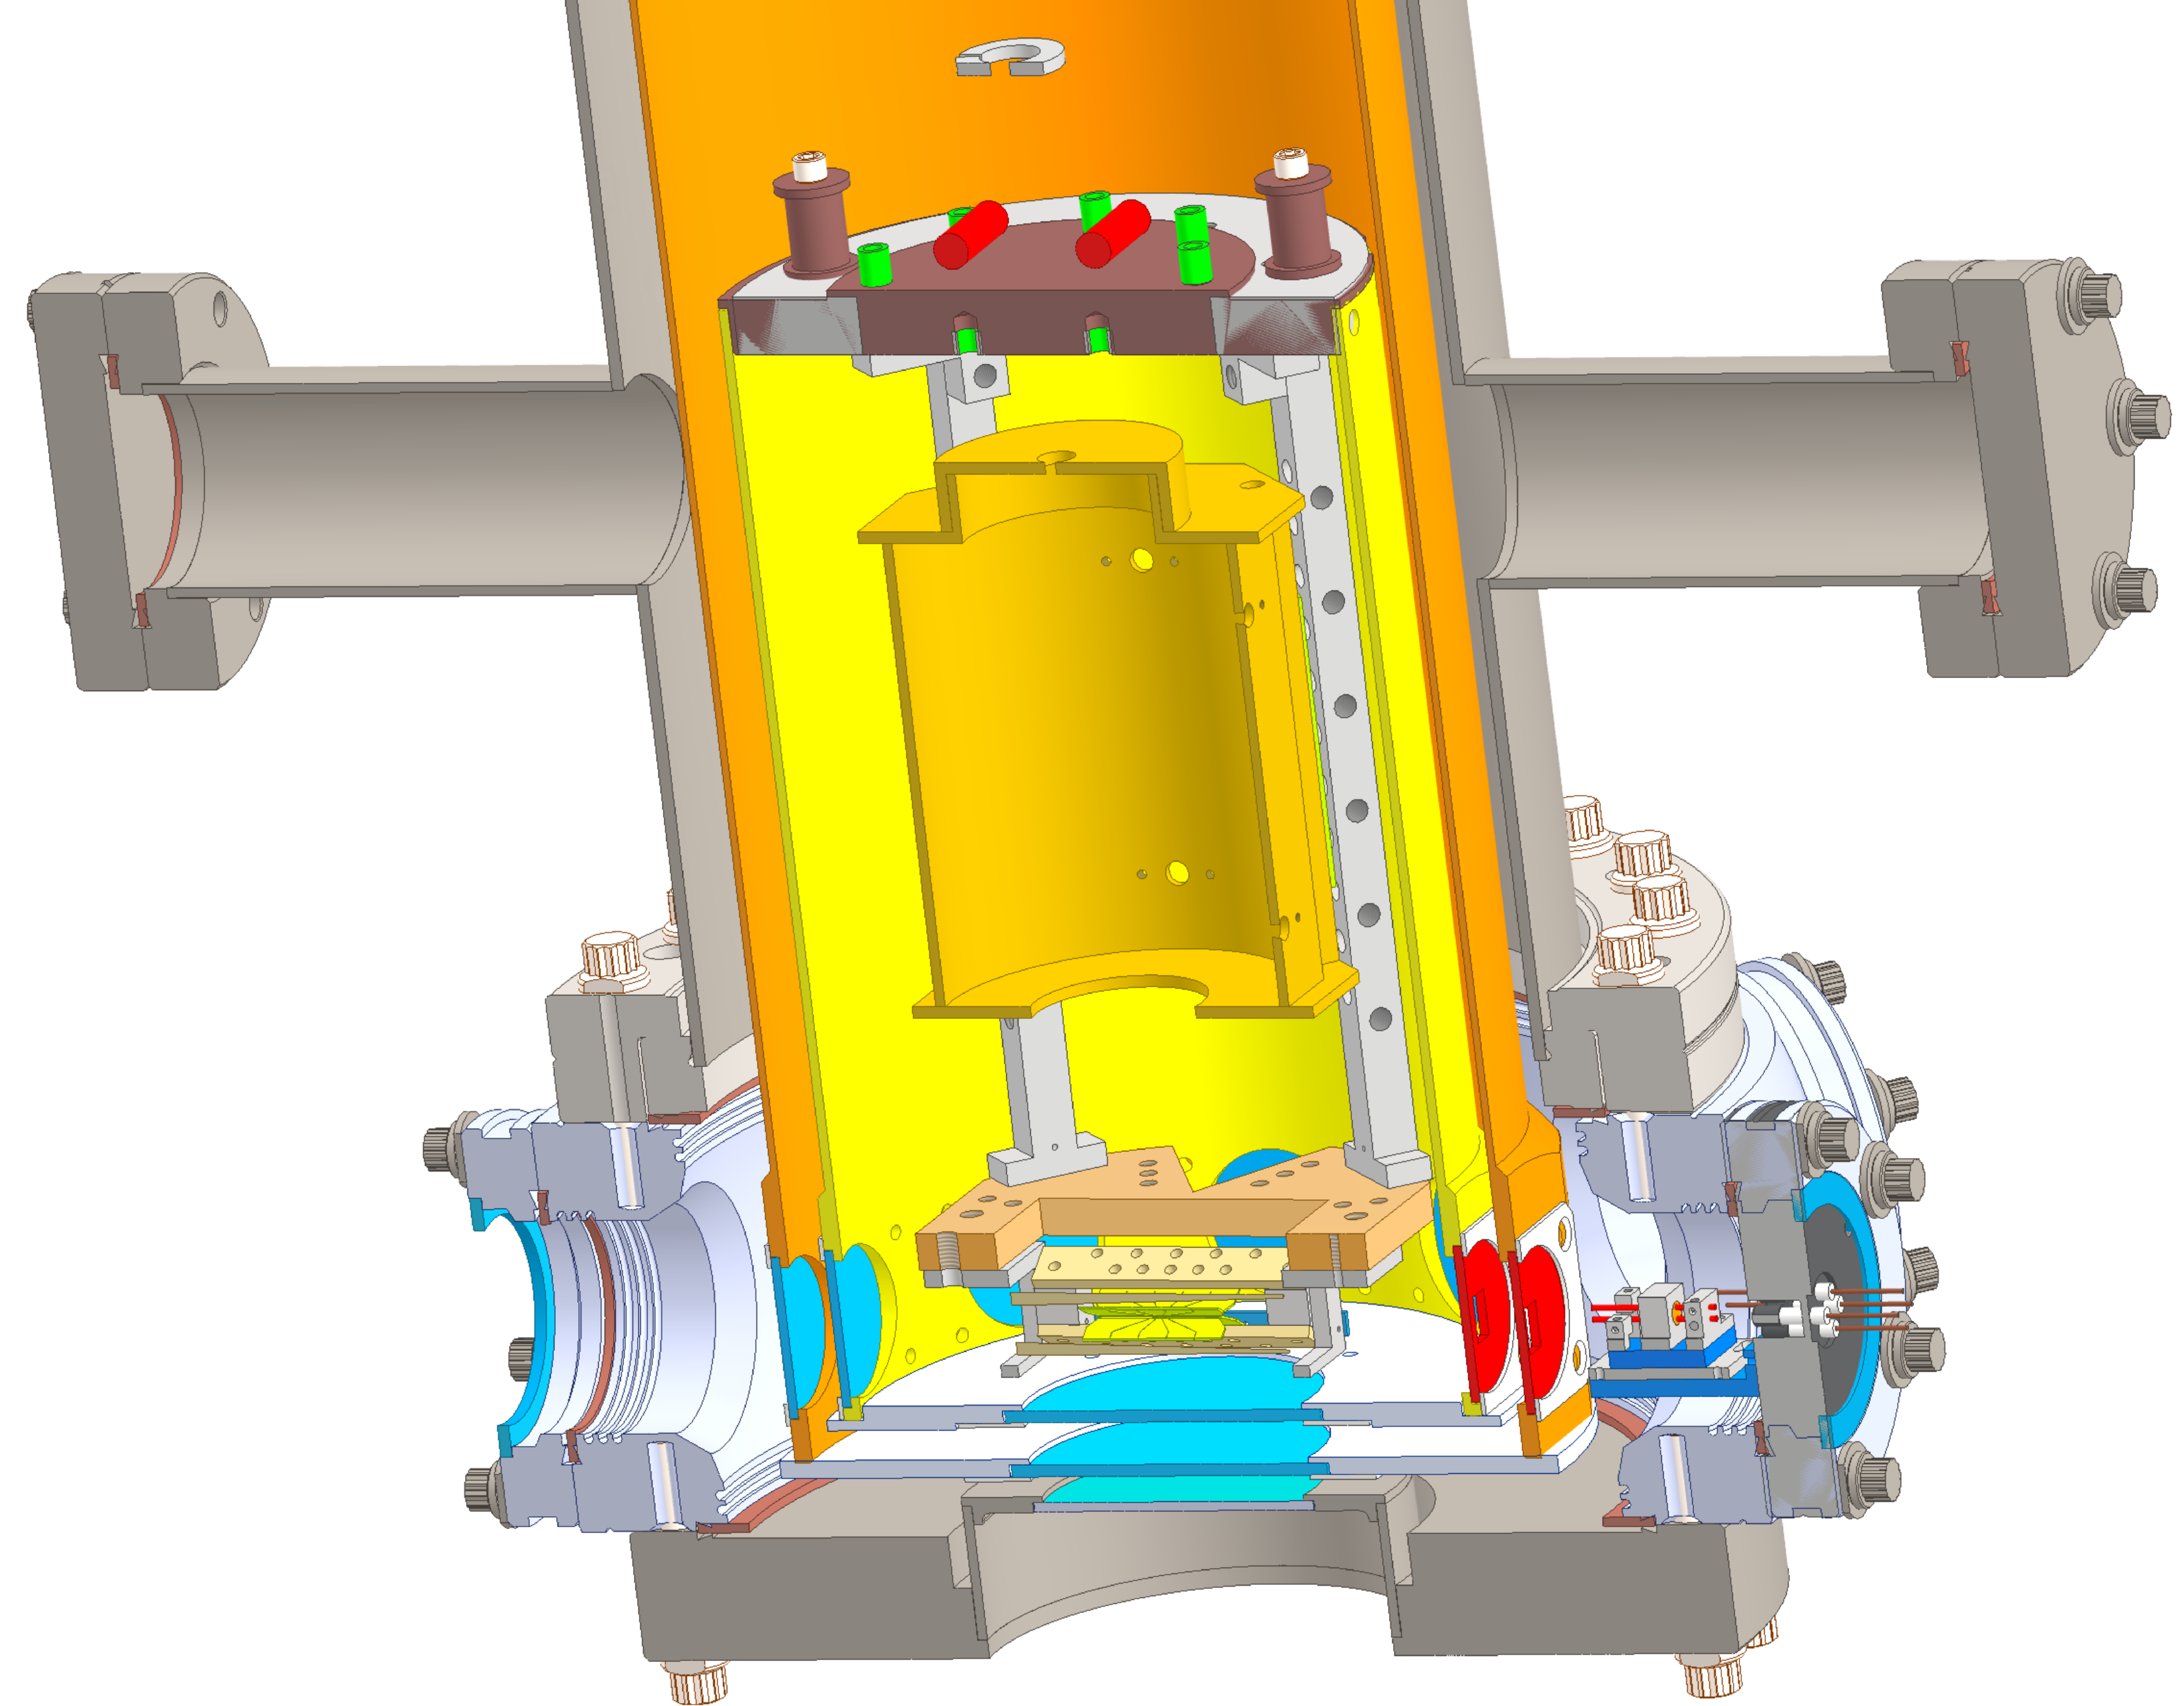
\includegraphics[width=0.4\linewidth]{fig_3_cryostat_b.pdf}}
    \subcaptionbox{The top view of ion trap and vacuum chamber.\label{fig:cryostat_c}}
    {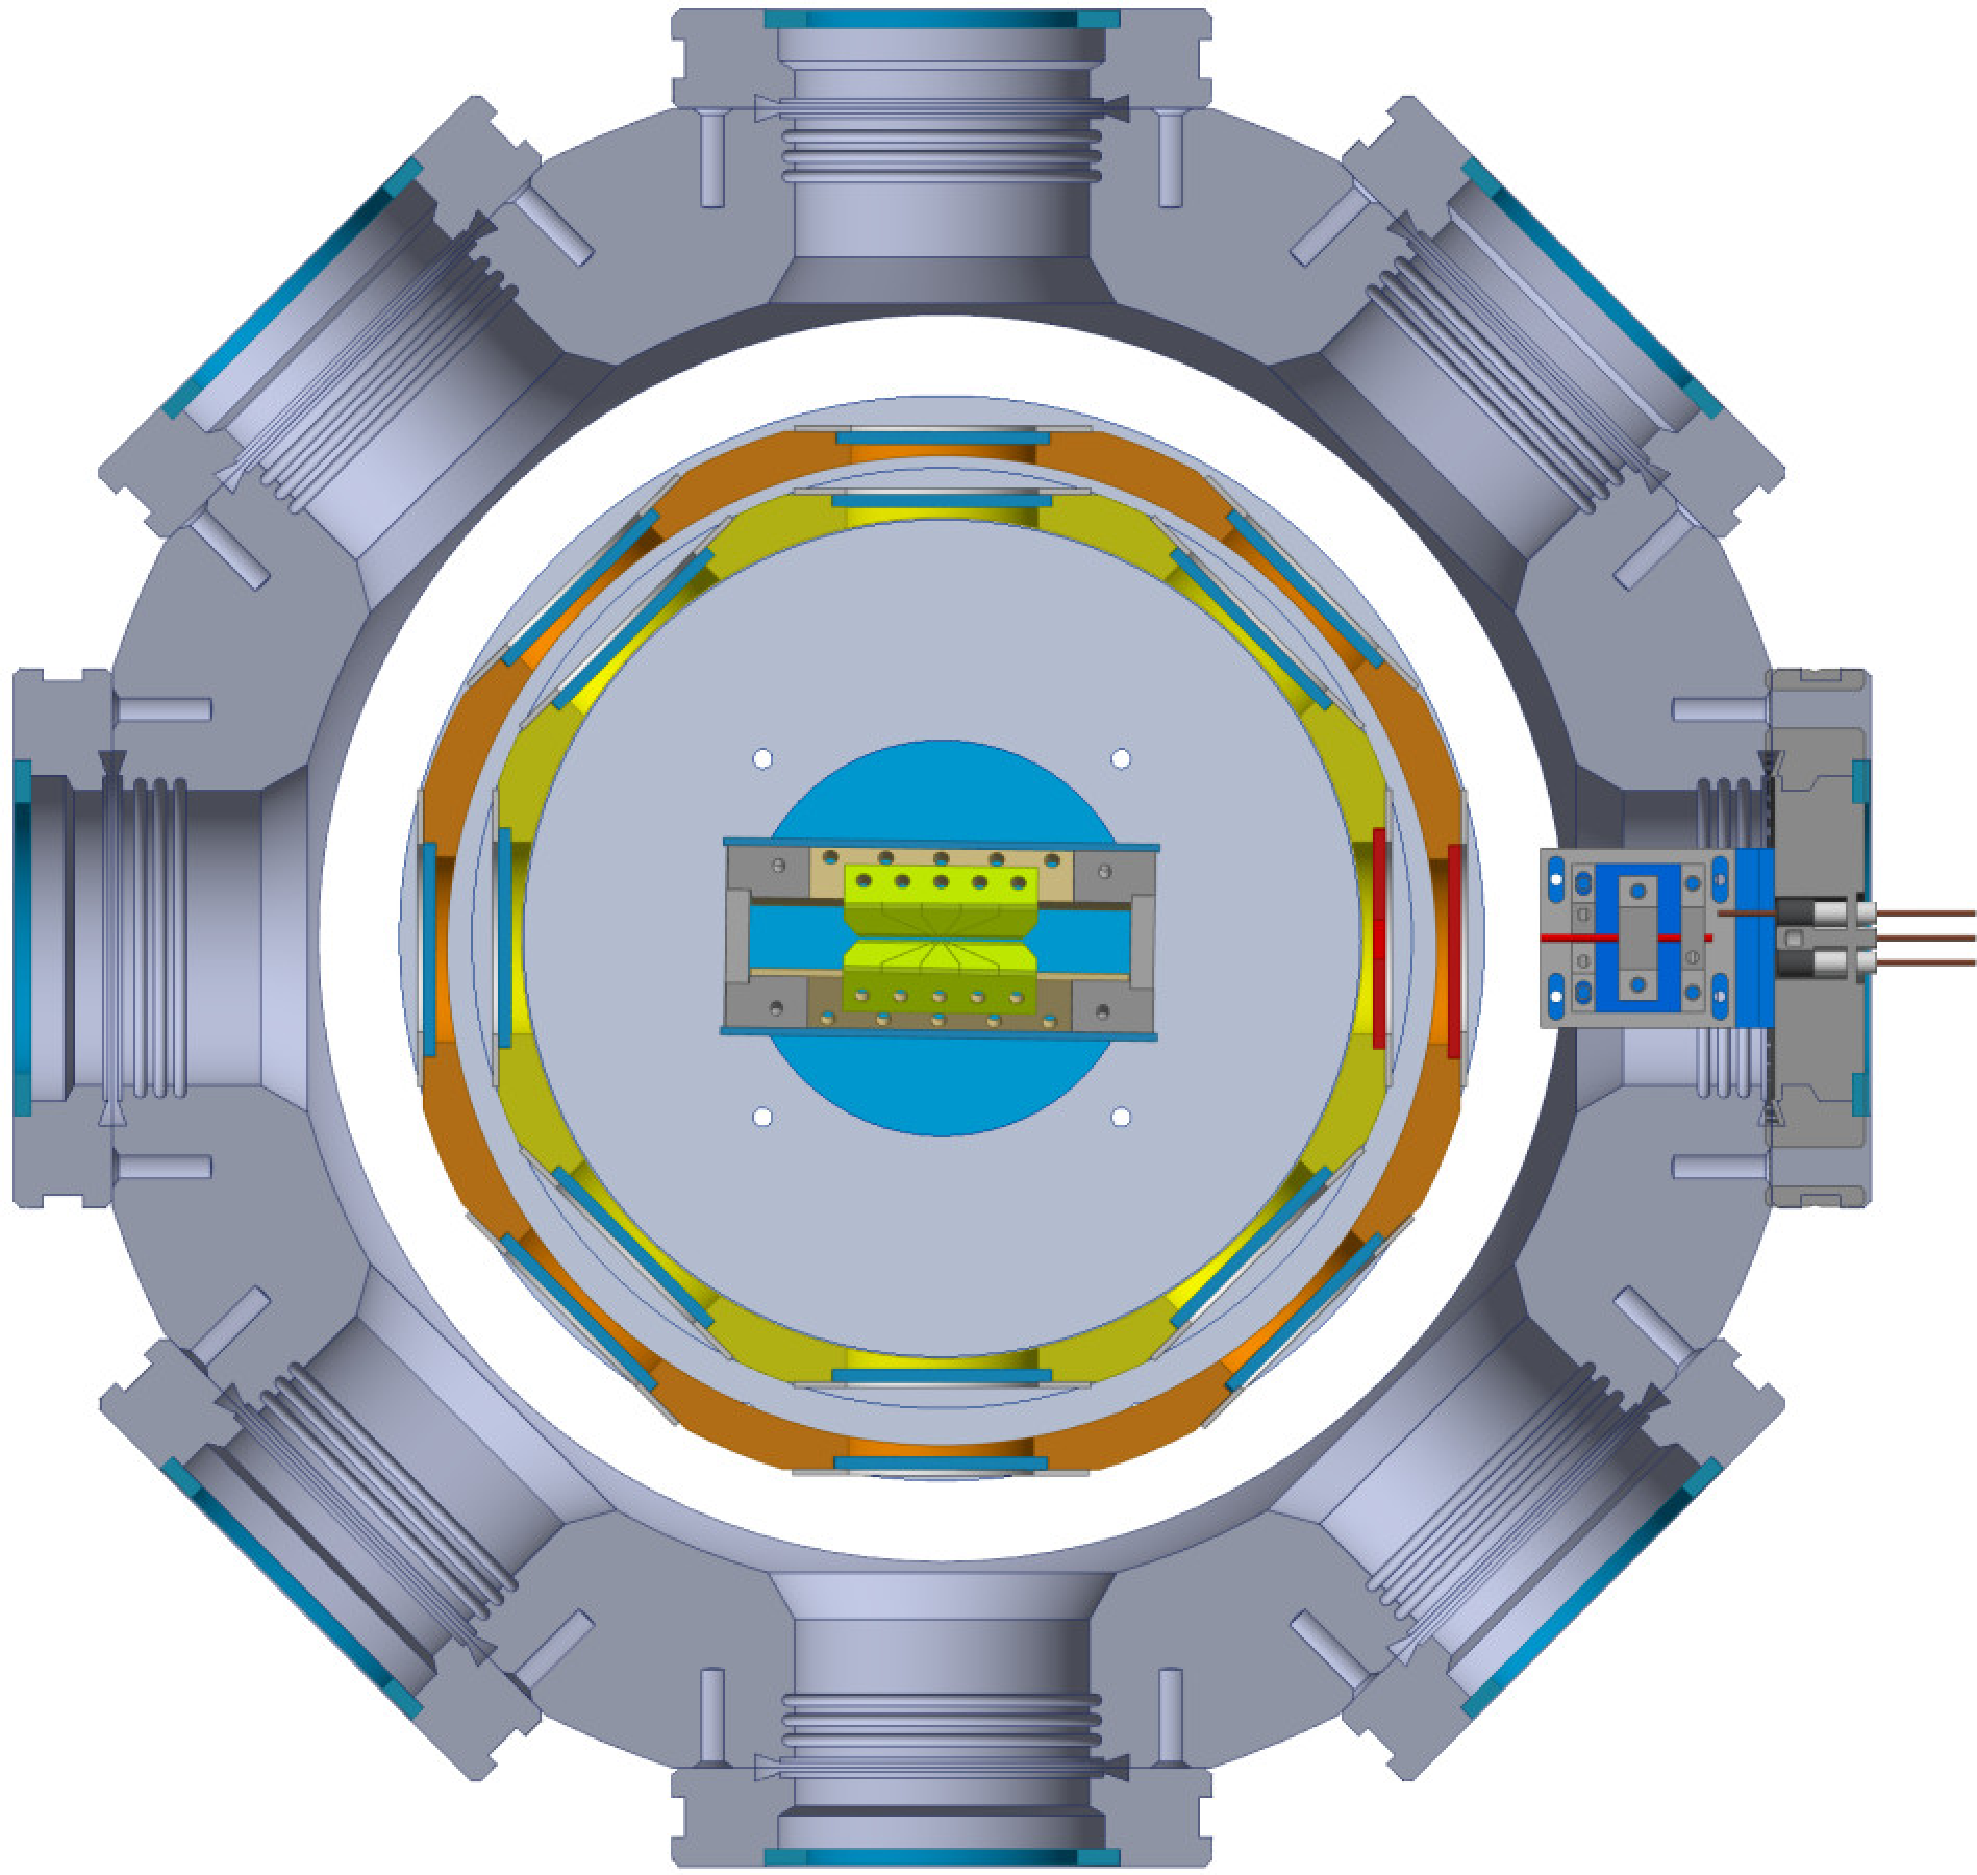
\includegraphics[width=0.4\linewidth]{fig_3_cryostat_c.pdf}}
    \caption{The design and related information of the cryostat.}
    \label{fig:cryostat}
\end{figure}

Although the refrigeration capacity of the 4 K stage in the cold head reaches 1.5 W, the cooling capacity of the sample mount in the vacuum chamber, which is directly available to the user, is much lower. The reduction of the cooling capacity comes from the heat conduction between the 4 K stage and the sample mount and the heat leakage from the environment. In order to improve the heat transfer between the 4 K stage and the sample mount, we can increase the surface area of the heat exchanger, we can also fill the exchange gas space with sufficient helium gas, and it is necessary to use oxygen-free copper to produce thermally conductive parts. In our experiments, we use auto gas charging system to stabilize the helium pressure in the exchange gas space at a fixed positive pressure. It is worth noting that the rubber bellow loses its vibration isolation function under negative pressure, and the life of the rubber bellow is reduced. The auto gas charging system was designed by PHYSIK and is based on the principle of using a PLC to read the helium pressure gauge and control the opening and closing moments of the helium valves, which will eventually stabilize the helium pressure gauge at 1.03 bar. There are two helium valves to control the helium inlet and outlet, and one safety value to allow excess helium to escape, preventing the bellow from bursting when the auto gas charging system is not working. The temperature stabilize system is a kit we purchased from Janis Inc. and consists of a thermometer, heater and temperature controller. The thermometer (DT-670-CU-HT-1.4H) is located inside the sample mount in the vacuum chamber and has a measurement range of 1.4-500 K, covering the cryostat operating range of approximately 4-300 K. The heater is a 25 $\Omega$ resistor very close to the thermometer. The DC lines of the heater and the thermometer are connected to the temperature controller (Model 26 from CryoCon) on the instrument rack via a DC feedthrough on the vacuum chamber. In low temperature operation, the temperature of the sample mount can be stabilized at $6 \pm 0.05$ K for a long time by setting the appropriate PID parameters, as shown in Fig~\ref{fig:cryostat_temperature}. The output power of the heater is about 350 mW, which means that the refrigeration capacity of the sample mount has a margin of 350 mW.

\begin{figure}
    \centering
    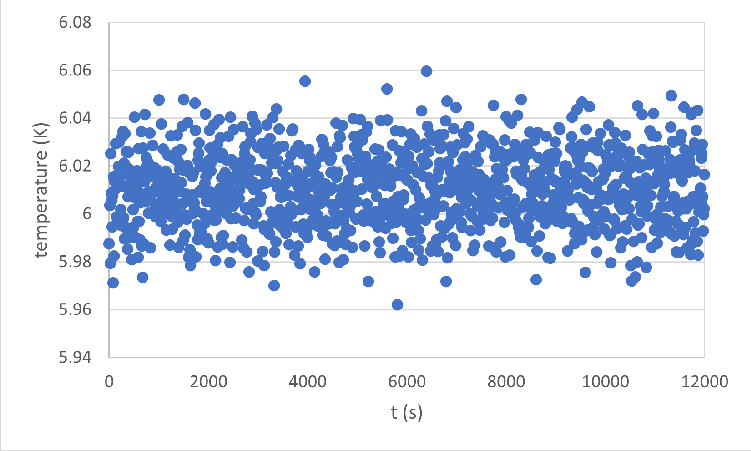
\includegraphics[width=0.7\linewidth]{fig_3_cryostat_temperature.pdf}
    \caption{The stablized temperature of the sample mount.}
    \label{fig:cryostat_temperature}
\end{figure}

The auto gas charging system and the temperature stabilize system are the key systems for the long-term stability of the cryostat. Although the temperature of This cryostat has almost no drift, we can observe that the trap can shift $\pm 1$ $\mu$m during the experiment. The operation to avoid the effects of such position shifts by frequent calibration of the system parameters is very complicated, so this instability can be fatal for an experimental system. The long drift of the sample mount comes from the mechanical structure of the cryostat. The auto gas charging system can only stabilize the helium pressure near the rubber bellow, and the 40 K stage and 4 K stage of the cold head are not stabilized. Therefore, the pressure and temperature in the contact part of the vacuum chamber and the exchange gas space cannot be stabilized for a long time. However, this part is the support point of the sample mount, so the sample mount will be disturbed by these external environmental changes. We can consider fixing the sample mount to the room temperature area of the vacuum chamber, which will not move if the laboratory environment is stable, but this will inevitably increase the heat leakage from the room temperature area. In our experiments, we first pumped the vacuum chamber to $1 \times {10}^{-6}$ mbar at room temperature using the Turbo Pump, then activated the NEG-Ion Pump for about 2 hours, and at the end of the operation the vacuum chamber vacuum level dropped to $1 \times {10}^{-8}$ mbar. The vacuum chamber can reach a vacuum level of $3 \times {10}^{-10}$ mbar with the effect of the cryo-pump.



\section{Helical resonator and segmented blade trap}

The blade trap forms a capacitor of approximately 6 pF. In order to drive this capacitor, i.e. to apply a high voltage signal to it, we need a larger helical resonator to form the LC oscillation circuit and to achieve impedance matching. The two components are therefore closely linked. The helical resonator and the blade trap are both located inside the 4 K shield of the vacuum chamber. The helical resonator is fixed underneath the sample mount and then the blade trap is fixed underneath the helical resonator. This ensures that the helical resonator and the blade trap are very close to each other and that their temperatures are equally stable. At the same time the low temperature allows the resistance in the oscillator circuit to be significantly reduced, which helps to increase the quality factor of the oscillator circuit. The helical resonator and the blade trap are used as a single unit and its input and output are achieved via RF and DC electric feedthrough.

\subsection{Design of helical resonator}

\begin{figure}
    \centering
    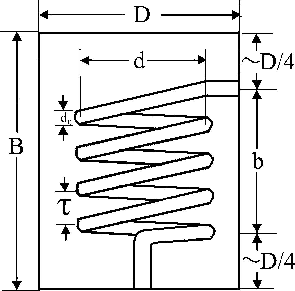
\includegraphics[width=0.5\linewidth]{fig_3_outline_design_of_a_helical_resonator.pdf}
    \caption{The outline design of a helical resonator.}
    \label{fig:outline_design_of_a_helical_resonator}
\end{figure}

The circuit models for the helical resonator and the blade trap have been well studied. In practice, we have developed a very mature design procedure with a high quality factor, choosing only two parameters $ b / d $ and $ d / D $ to optimise the performance of the helical resonator with the quality factor as the objective function. We can calculate the loading frequency in the empirical parameter regime using the trap capacitance and the quality factor. Typically, $ b / d \approx 1.5 $ and $ d / D \approx 0.5 $ is a good choice, and if the loading frequency meets our requirements we will try to choose the highest quality factor around this parameter range, as shown in Fig~\ref{fig:outline_design_of_a_helical_resonator}. A two-wire spiral resonator is much more complex than a single-wire spiral resonator because of the coupling between the two coils. However, for the sake of simplicity we are still using the model and we can achieve an accuracy of about $\pm 5$ MHz. To ensure that the phase and amplitude of the two coils are the same, we use a parallel capacitor, which is shorted when connected to the RF feedthrough, with a capacitance of approximately 300 nF. The two-wire design is designed to help minimise micro-movements by applying a DC voltage to the RF electrodes, so we need to ensure that the RF signal on the coil is grounded and the DC voltage is not, this is achieved by a 300 nF capacitor connected to the shield. In addition, we added an RC filter before the DC voltage was connected to the coil.

\subsection{Circuit diagrams of the helical resonator and the blade trap}

\begin{figure}
    \centering
    \subcaptionbox{Circuit diagrams of the helical resonator.\label{fig:circuit_diagram_helical_resonator}}
    {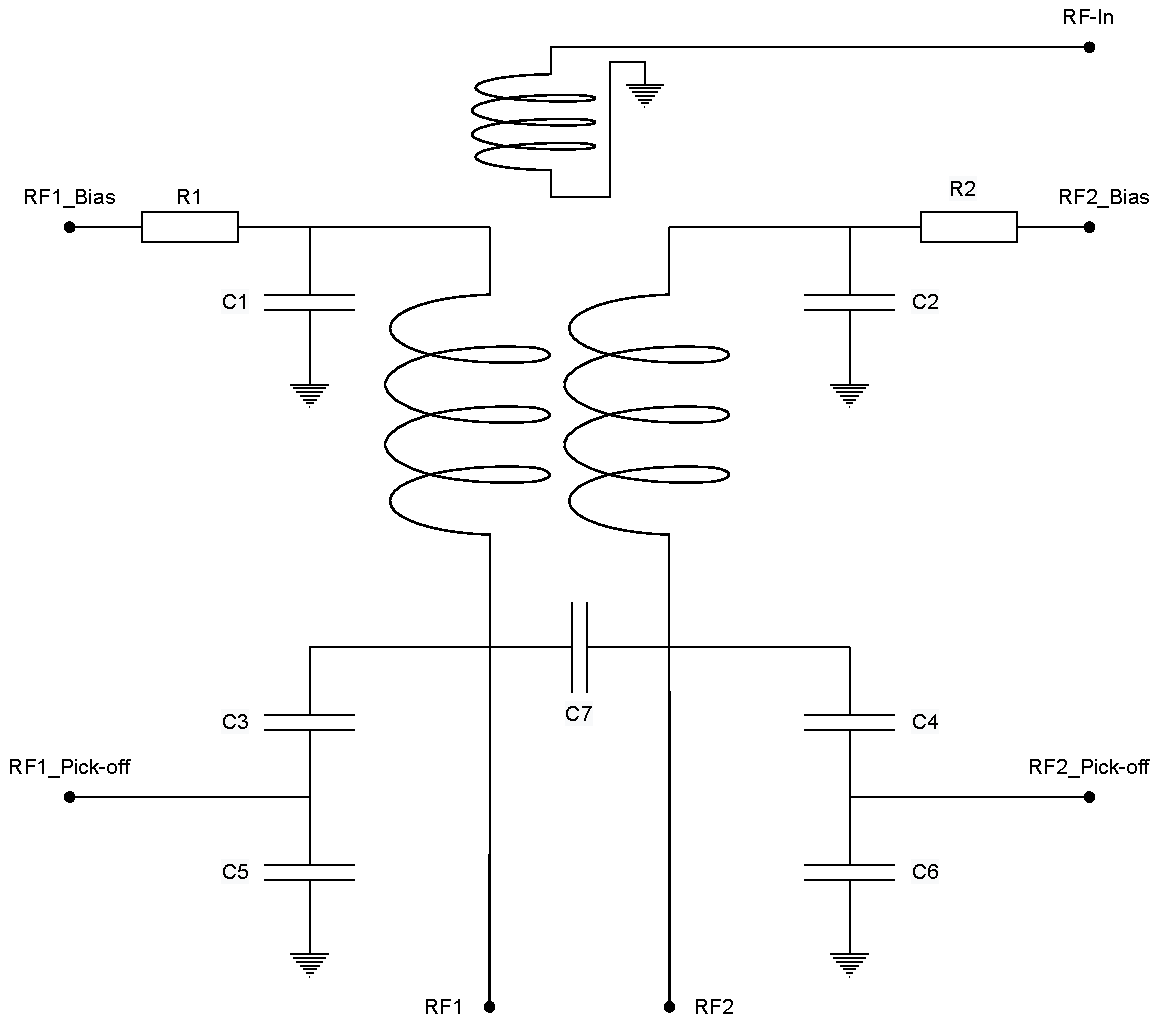
\includegraphics[width=0.5\linewidth]{fig_3_circuit_diagram_helical_resonator.pdf}}
    \subcaptionbox{Circuit diagrams of the blade trap.\label{fig:circuit_diagram_blade_trap}}
    {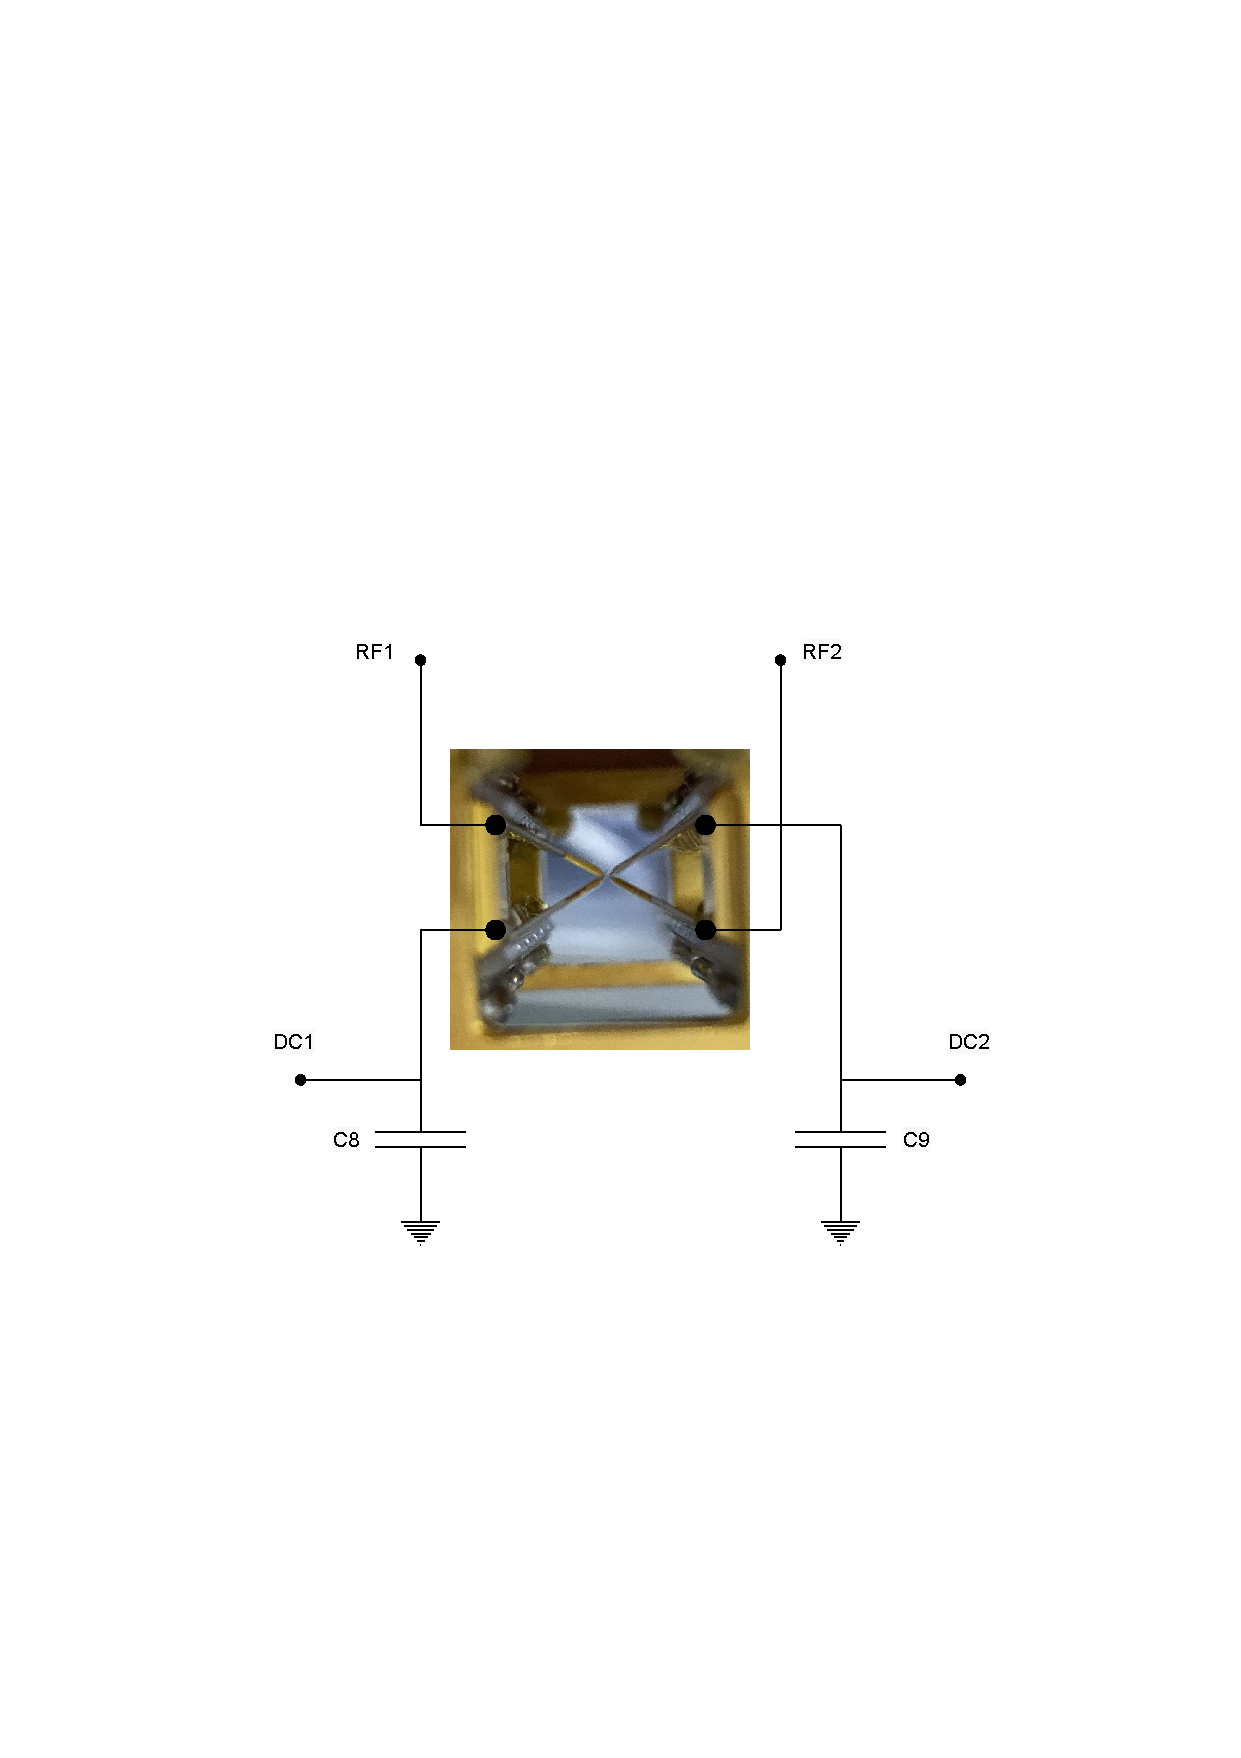
\includegraphics[width=0.3\linewidth]{fig_3_circuit_diagram_blade_trap.pdf}}
    \caption{Circuit diagrams of the helical resonator and the blade trap.}
    \label{fig:circuit_diagram}
\end{figure}

To facilitate our understanding of the circuit structure of the helical resonator and the blade trap, Fig~\ref{fig:circuit_diagram_helical_resonator} shows their equivalent circuit diagrams. In Fig~\ref{fig:circuit_diagram_blade_trap}, an external RF signal (RF-In) is fed to a small antenna. The antenna is coupled to a double bifilar helical copper wire, which is short-circuited by a large capacitor (C7, 330nF). The two RF bias signals (RF1 Bias and RF2 Bias) are supplied by the AD5791 and pass through an RC filter consisting of a resistor (R1, R2, 10 $k\Omega$) and a capacitor (C1, C2, 330 nF) to add a DC bias to the respective RF signal. The two capacitively coupled signals (RF1 Pick-off, RF2 Pick-off) can be coupled to a 1\% RF resonant signal. The voltage divider circuit uses a small capacitor (C3, C4, 0.2 pF) and a large capacitor (C5, C6, 20 pF) in series. The signal from the two pairs of DC electrodes on the blade trap (DC1, DC2) is grounded through large capacitors (C8, C9, 820 pF).

\begin{table}
    \centering
    \caption{Table of electronic components in the circuit diagrams.}
    \begin{tabular}{p{0.15\linewidth}p{0.1\linewidth}p{0.3\linewidth}p{0.3\linewidth}}
        \toprule
        Component & Value        & Model            & Parameters                   \\
        \midrule
        Resistor  & 10 $k\Omega$ & RNCF1206TKY10K0  & RES 10K OHM 0.01\% 1/4W 1206 \\
        Capacitor & 0.2 pF       & VJ1111D0R2VXRAJ  & 1.5KV                        \\
        Capacitor & 20 pF        & 800B200JT500XT   & CAP CER  500V C0G/NP0 1111
        \\
        Capacitor & 820 pF       & C0805C821JCGACTU & CAP CER  500V C0G/NP0 0805   \\
        Capacitor & 330 nF       & C2220C334J1GACTU & 100V NP0
        \\
        \bottomrule
    \end{tabular}
\end{table}

\subsection{Assembly of the helical resonator}

The material used for the body of the helical resonator is oxygen-free copper, which is characterised by its very low resistivity and high thermal conductivity. The low resistivity helps to obtain a high quality factor, but the oxygen-free copper is susceptible to oxidation during processing, so the oxide film needs to be removed before assembly. After the helical resonator has been assembled, it needs to be placed in a vacuum enclosure to prevent oxidation.

\begin{figure}
    \centering
    \subcaptionbox{Assembly of the helical resonator antenna.\label{fig:assembly_of_helical_resonator_antenna}}
    {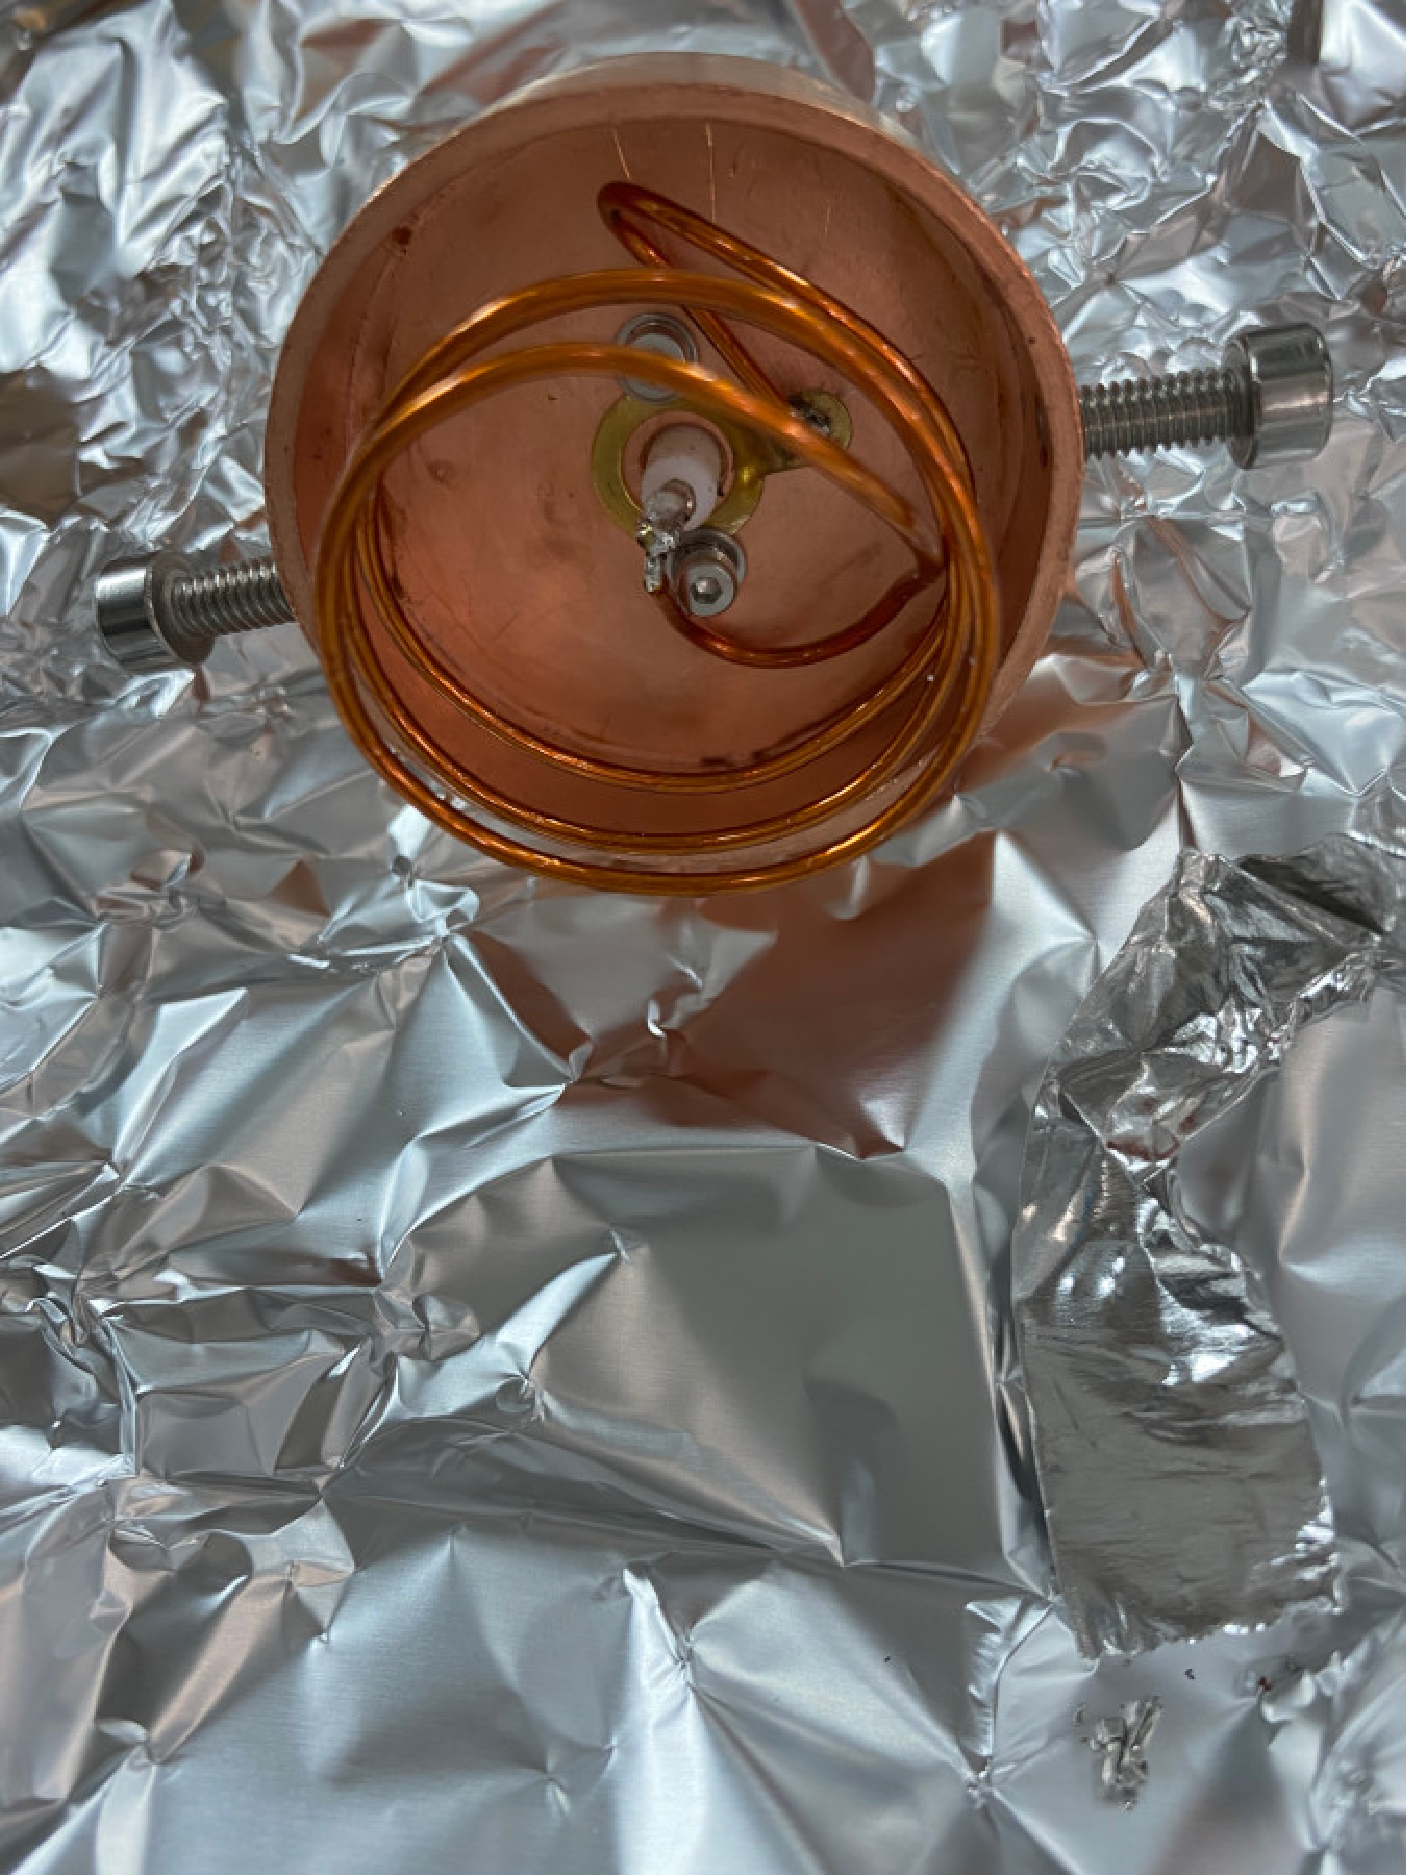
\includegraphics[width=0.4\linewidth]{fig_3_assembly_of_helical_resonator_antenna.pdf}}
    \subcaptionbox{Assembly of the main section.\label{fig:assembly_of_helical_resonator_copper}}
    {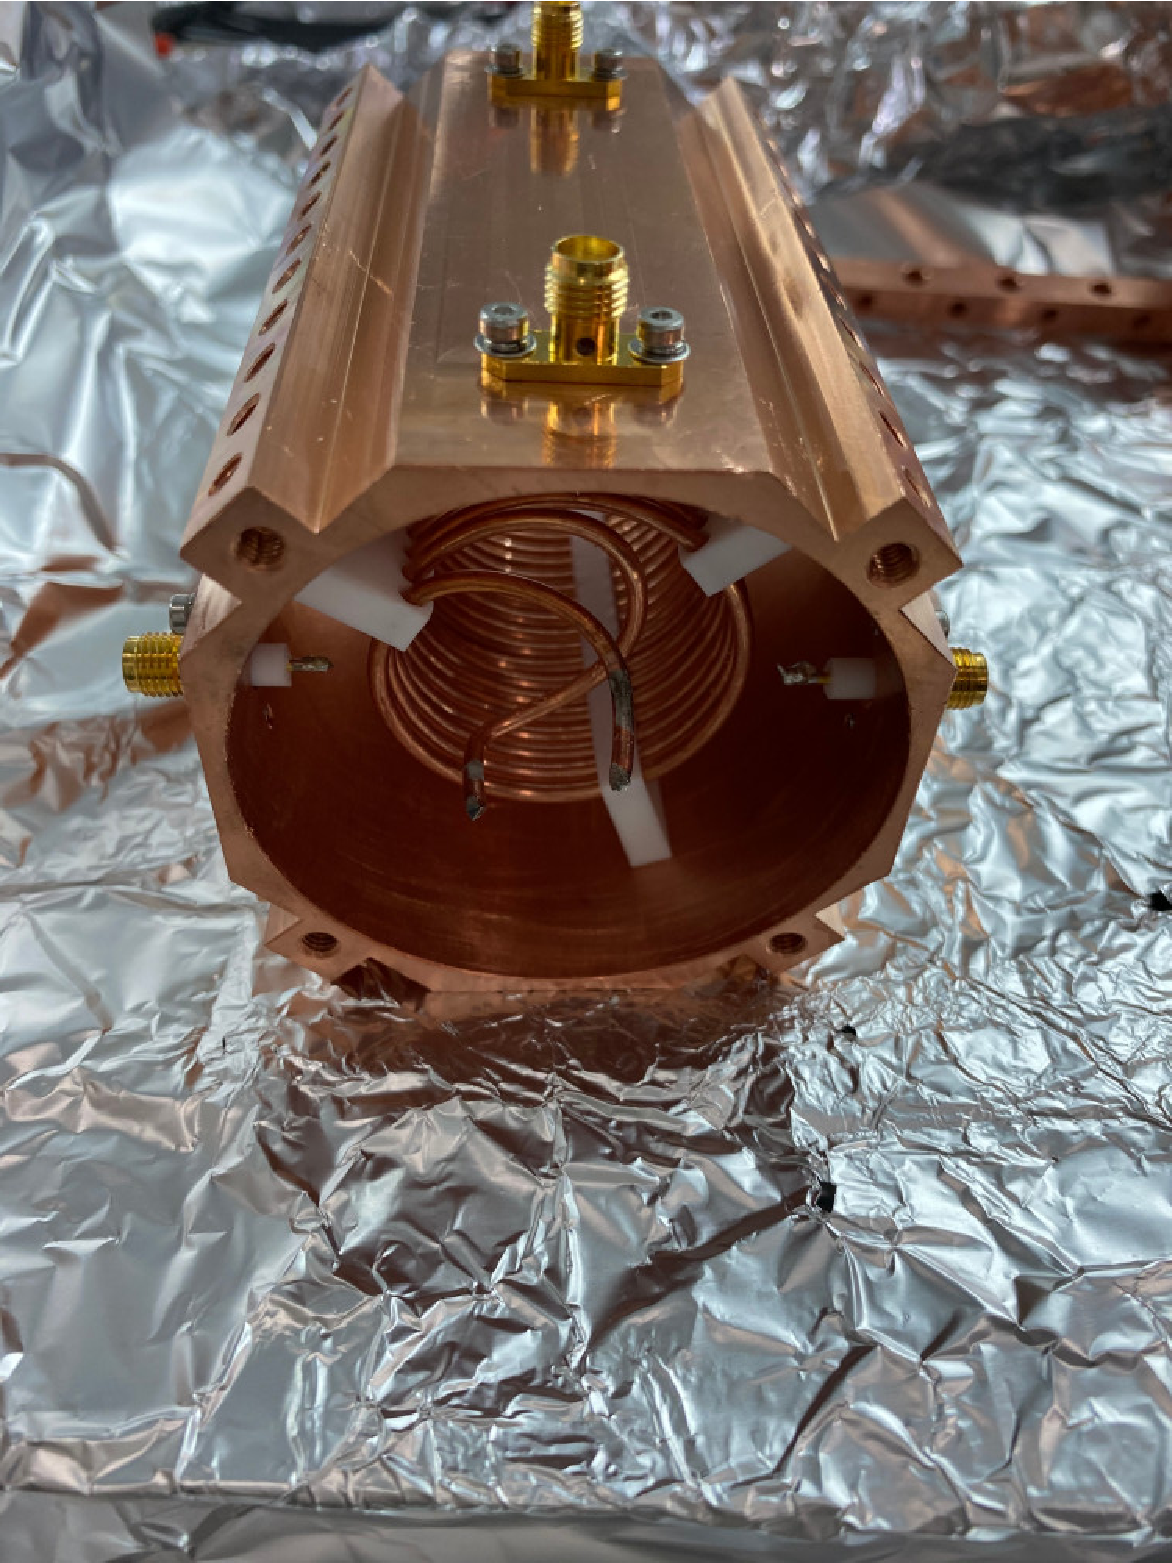
\includegraphics[width=0.4\linewidth]{fig_3_assembly_of_helical_resonator_copper.pdf}}
    \subcaptionbox{Assembly and soldering of the PCB.\label{fig:assembly_of_helical_resonator_pcb}}
    {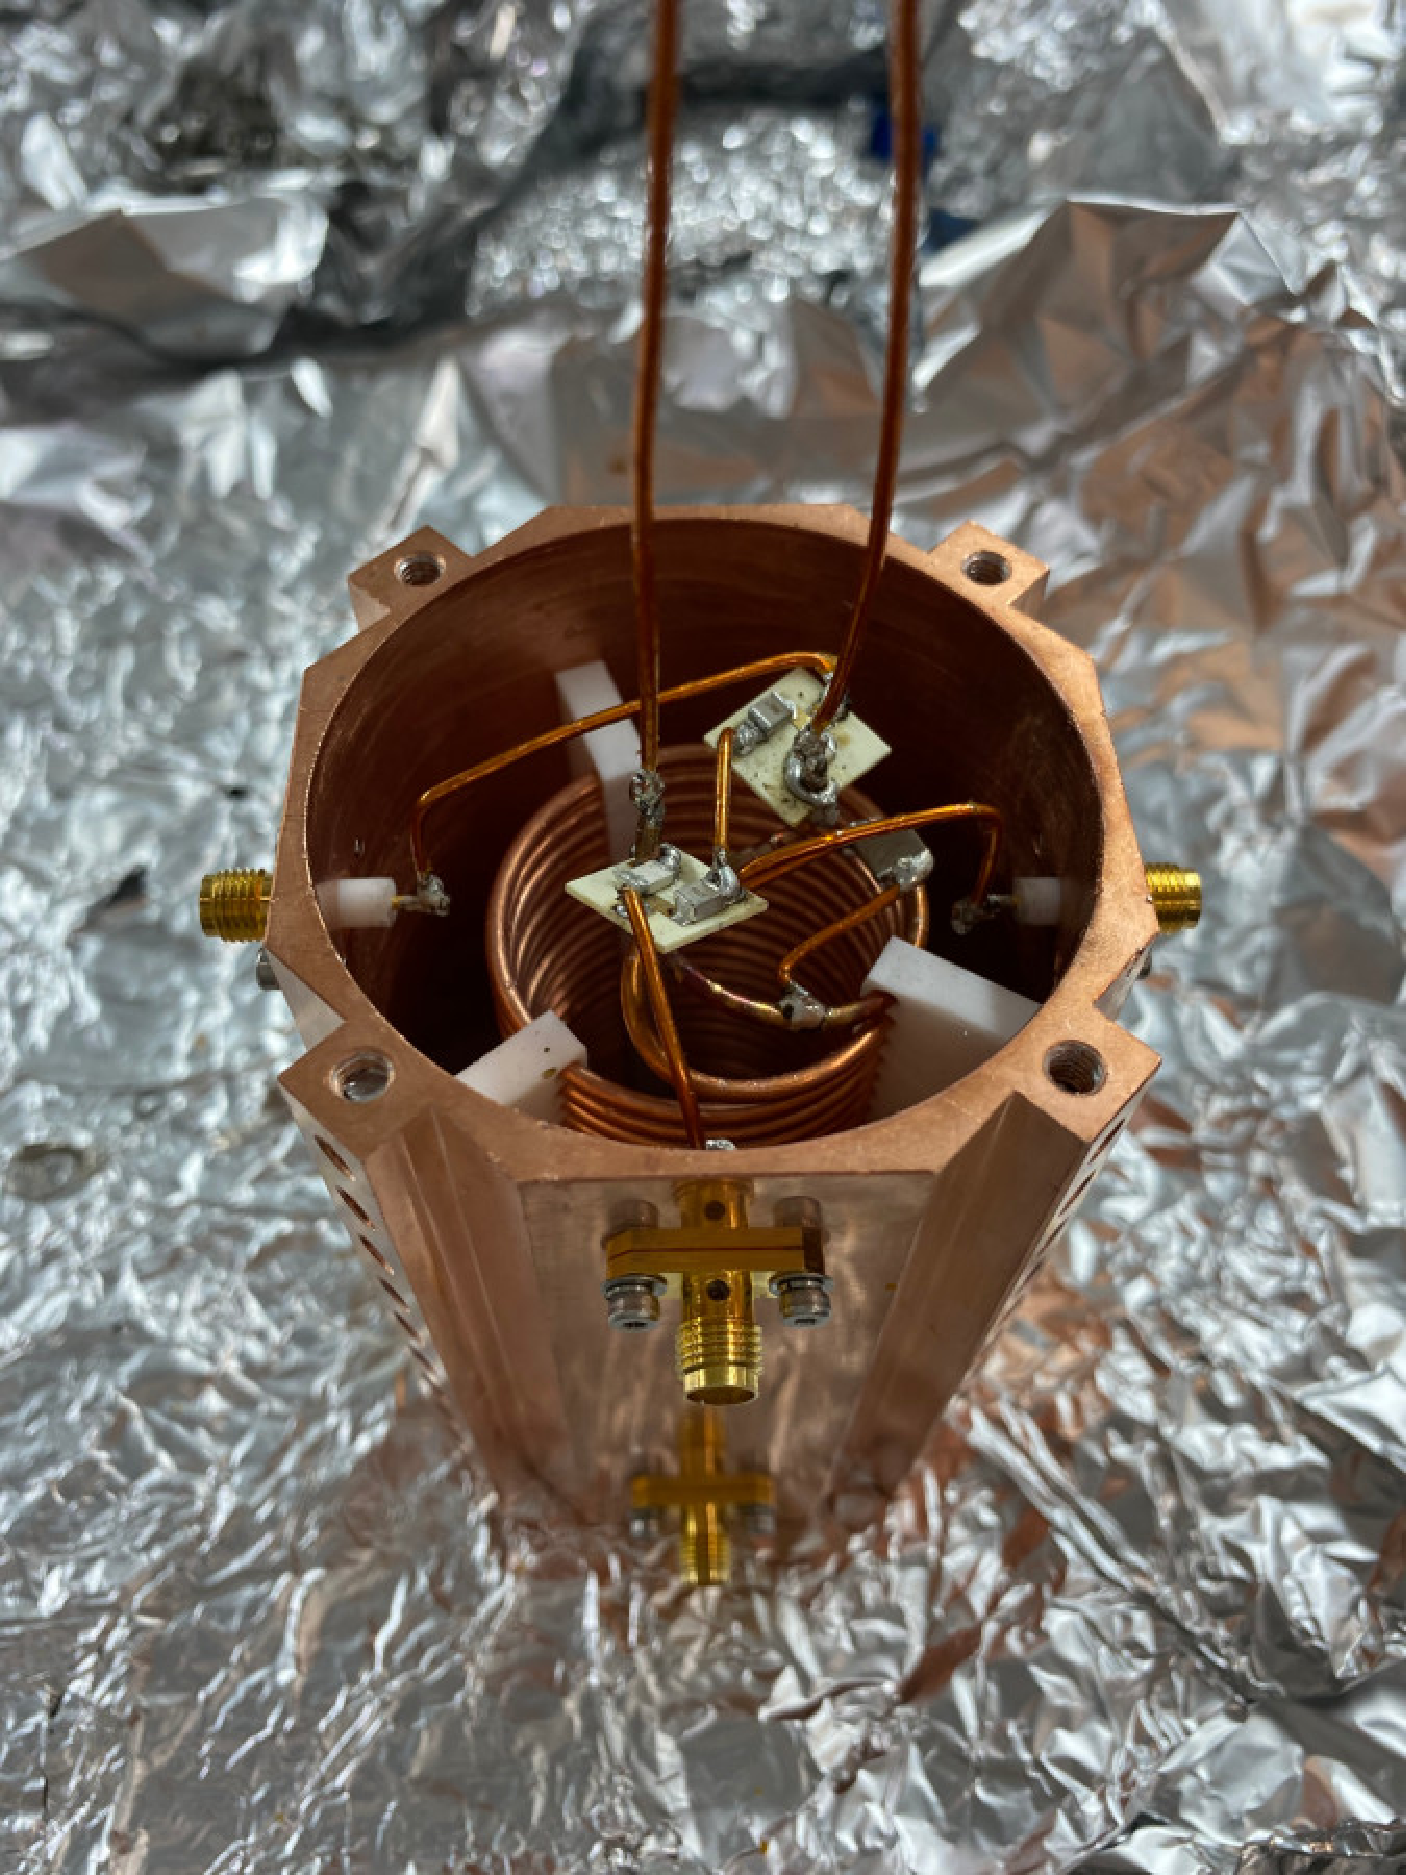
\includegraphics[width=0.5\linewidth]{fig_3_assembly_of_helical_resonator_pcb.pdf}}
    \caption{Assembly of the helical resonator.}
    \label{fig:assembly_of_helical_resonator}
\end{figure}

\begin{table}
    \centering
    \caption{Assembly procedures of the helical resonator.}
    \begin{tabular}{p{0.2\linewidth}p{0.7\linewidth}}
        \toprule
        Procedure    & Content                                                                                                                                                                                                                    \\

        \midrule
        Preservation & Oxygen-free copper components should not be left in the air for long periods of time and need to be placed in a vacuum enclosure.                                                                                          \\
        Clean        & Disassemble the helical resonator and take out the oxygen-free copper components individually into large beakers in preparation for sonication.                                                                            \\
                     & Sonicate them with acetone for 30 minutes and with ethanol for 5 minutes.                                                                                                                                                  \\
                     & Blow the components dry.                                                                                                                                                                                                   \\
                     & Soak them in organic acid for 5 minutes, where the surface oxide film can be observed to disappear and turn purplish red.                                                                                                  \\
                     & Remove residual organic acids from the surface by immerse them in plenty of distilled water.                                                                                                                               \\
                     & Wipe the surface of the oxygen-free copper components with paper, place them in a vacuum hood and evacuate the vacuum enclosure.                                                                                           \\
        Preparation  & Cut a number of thick wires into suitable length and trim off the insulation at both ends.                                                                                                                                 \\
                     & Prepare the PCB, capacitors, resistors, screw coil retainers, SMA connectors, copper plated components, indium foil, screw sets, spanners.                                                                                 \\
                     & Soak the capacitors, resistors and indium foil in acetone for 30 minutes and in ethanol for 5 minutes, sonicate the rest in acetone for 30 minutes and in ethanol for 5 minutes.                                           \\
        Test         & Measure the inductance of the helical resonator with an LCR meter. (1.50 $\mu$H and 1.41 $\mu $H.)                                                                                                                         \\
                     & Measure the scattering parameters of the helical resonator with a vector network analyzer.                                                                                                                                 \\
                     & The antenna position and pitch were adjusted to match the impedance when the helical resonator was unloaded. (f = 69.15 MHz, Q = 434.7 U, R = 50.90 dB.)                                                                   \\
                     & After the helical resonator is connected to the Trap, the antenna position and pitch are adjusted so that the impedance matches, and at this point the RC filter is connected. (f = 36.83 MHz, Q = 373.6 U, R = 28.05 dB.) \\
        \bottomrule
    \end{tabular}
\end{table}

The main parts of the helical resonator were machined according to the design parameters: the antenna cover, the top cover, the middle part, the bottom cover and the helical coils, which were then cleaned in the ultrasound machine using acetone and ethanol. After drying these parts with nitrogen and soaking them in organic acid for 5 minutes, it can be observed that the surface oxide film disappears and turns purplish red. We soak the parts in plenty of distilled water to remove the residual organic acid and then dry the parts with nitrogen. The cleaning of the parts of the main part of the copper tube is now complete. This part needs to be done carefully, as the oxide film on the helical resonator surface affects the quality factor.

We also need to prepare and clean the rest of the parts according to the design parameters to meet the ultra-high vacuum requirements. We then soldered the circuit components together using lead-free solder. The parts are then assembled with stainless steel screws, each requiring a resilient pad to prevent the screws from loosening at low temperatures.


\subsection{Assembly of blade trap}

The advantage of the blade trap is that it is easy to process and assemble, but the disadvantage is that the assembly error is higher compared to the surface trap or the monolithic trap, which causes an asymmetry in the electrostatic potential at the centre of the trap where the ions are located, i.e. a deviation from the linear trap configuration. When designing the blade trap for use in the cryostat, we need to take care that the material has a high thermal conductivity and that the connections between the components are sufficiently tight. In this way we can achieve the lowest temperatures on the blade trap. This helps to obtain a higher vacuum level and to extend the life of the ions.

\begin{figure}
    \centering
    \subcaptionbox{Assembly of the sapphire and indium film.}
    {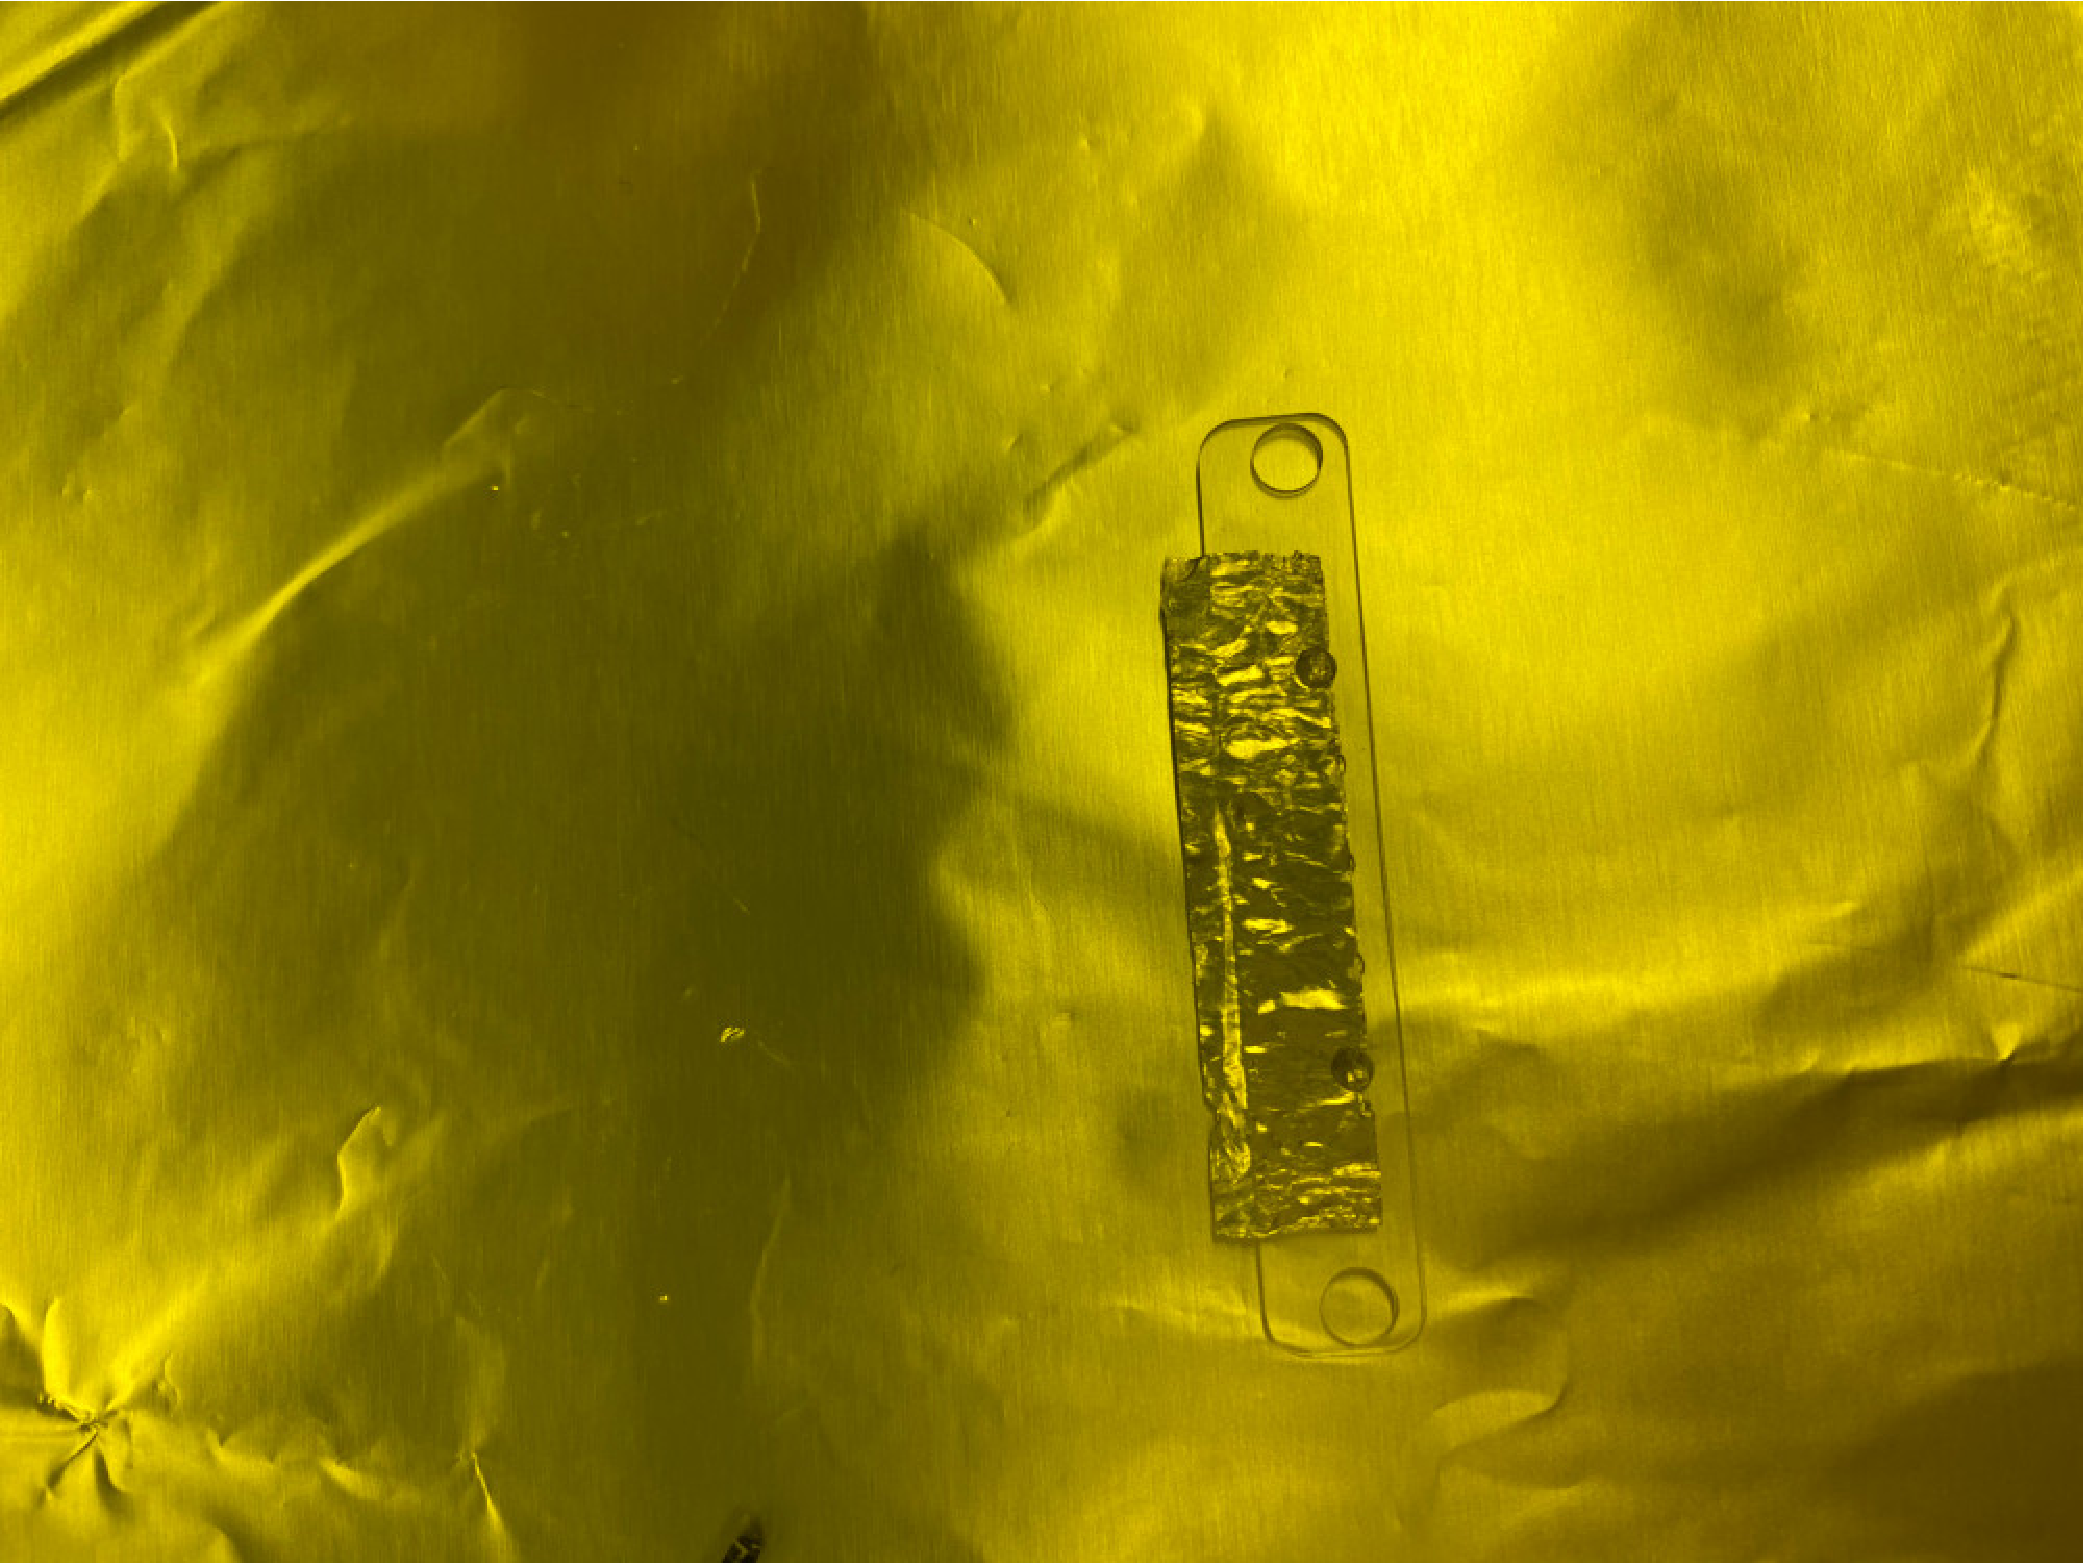
\includegraphics[width=0.4\linewidth]{fig_3_assembly_of_trap_sapphire.pdf}}
    \subcaptionbox{Assembly of the blade.}
    {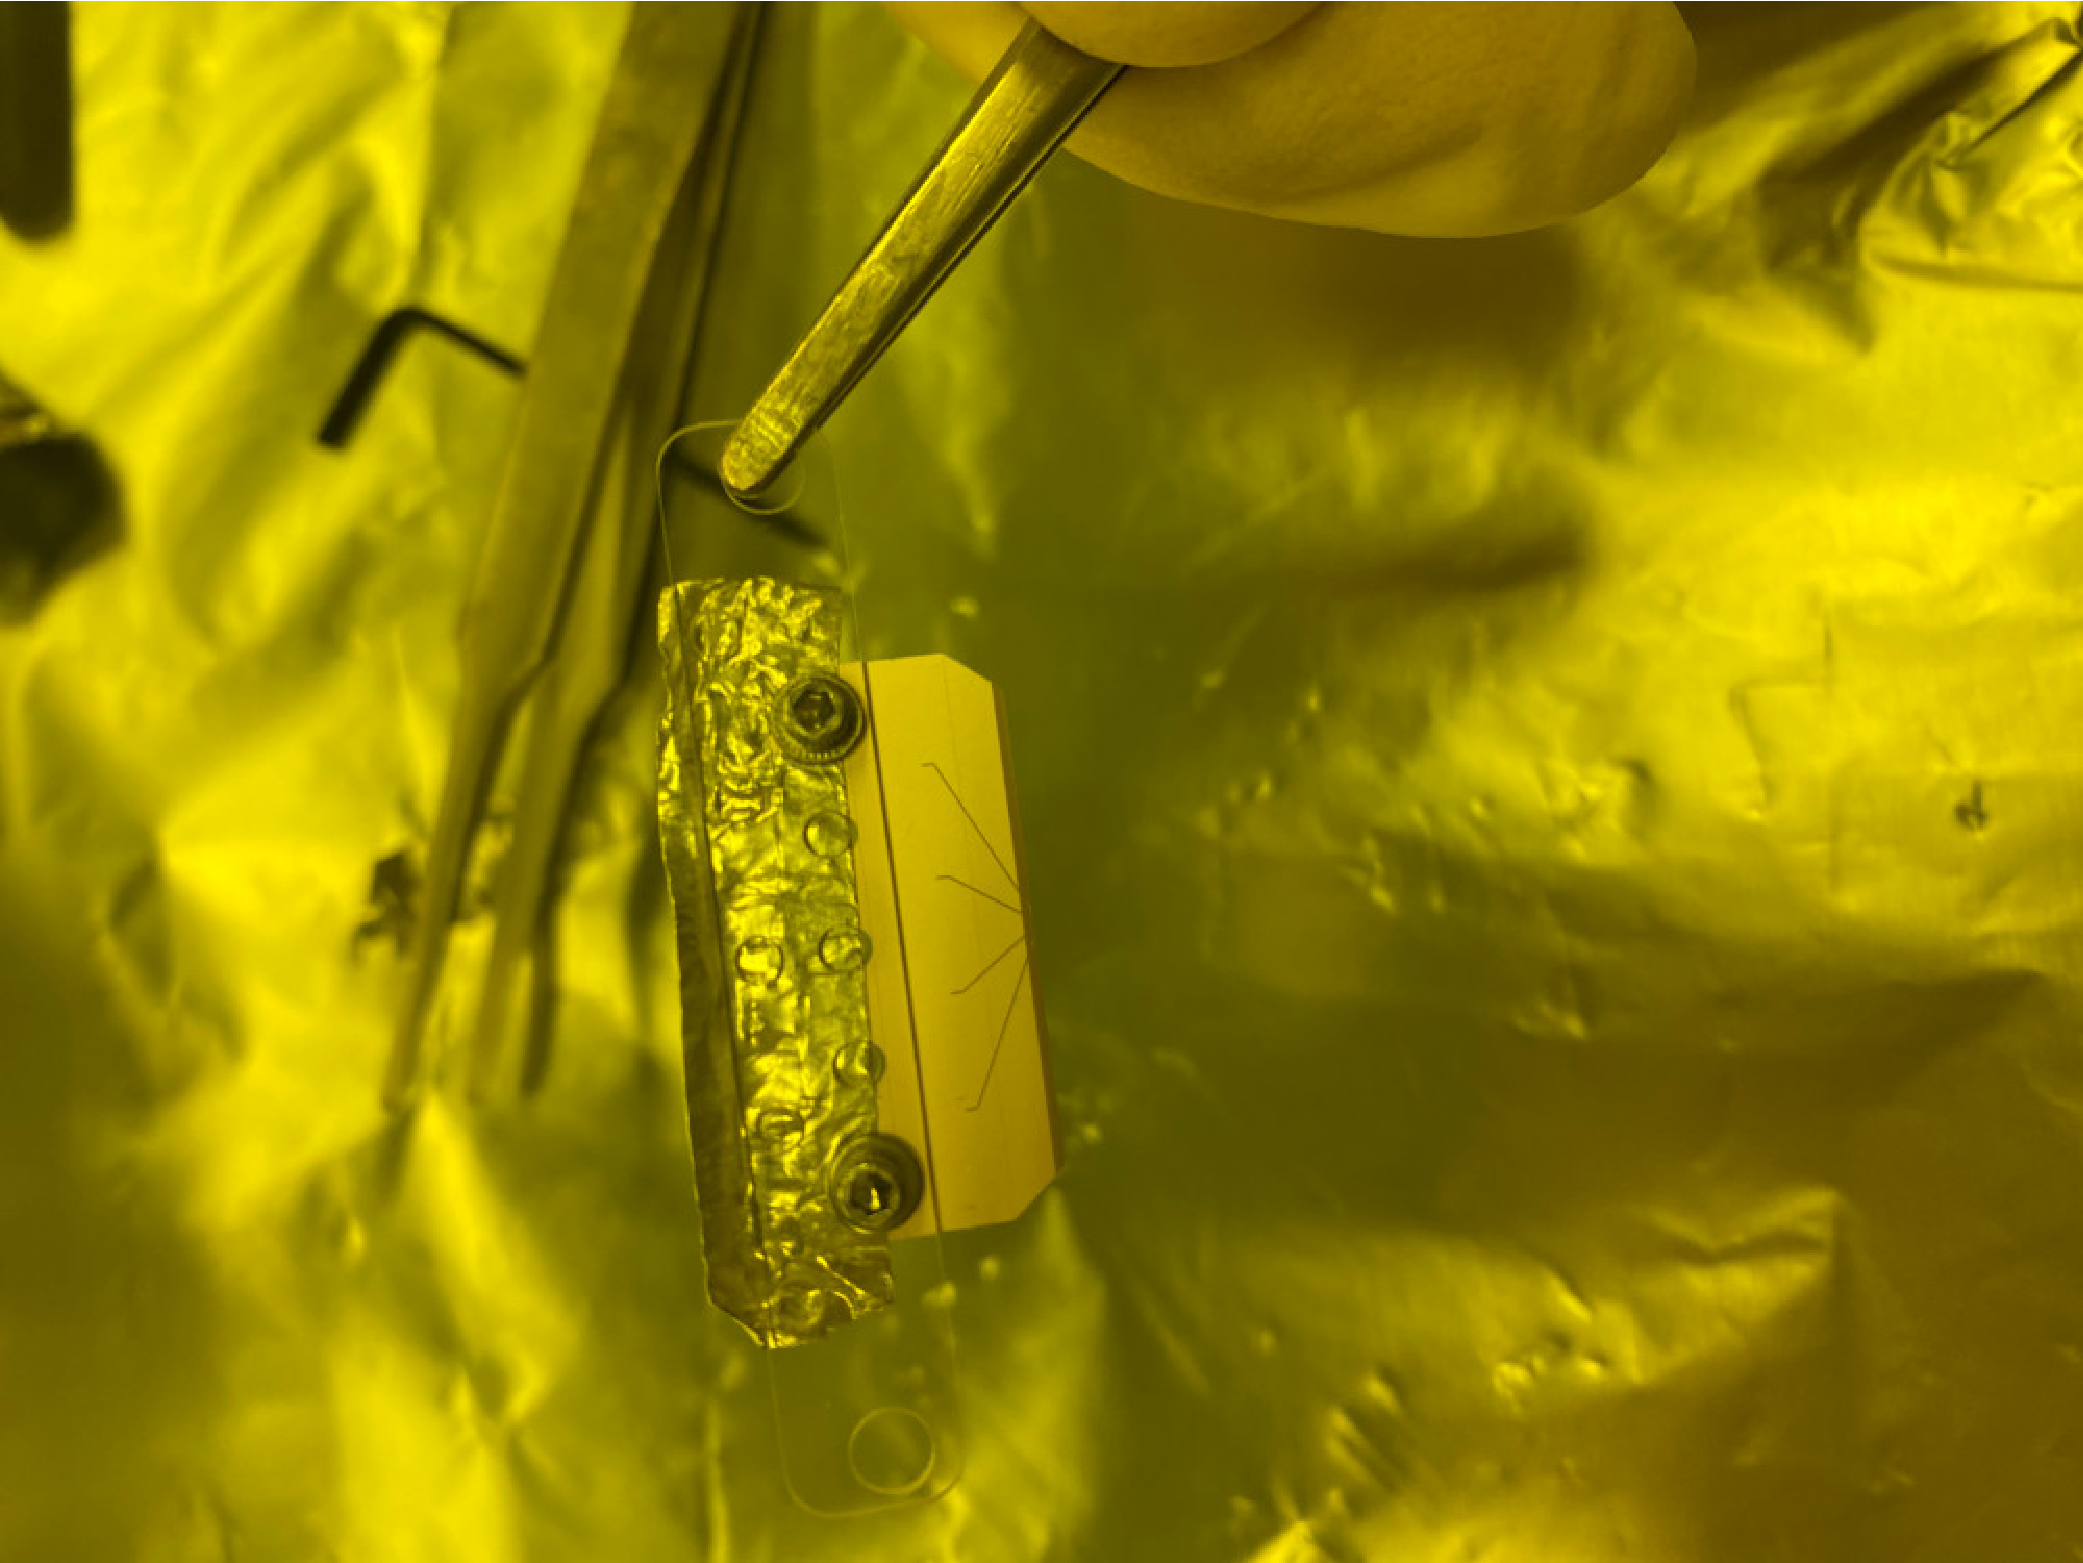
\includegraphics[width=0.4\linewidth]{fig_3_assembly_of_trap_blade.pdf}}
    \subcaptionbox{Assembly of the PCB and the gold ribbon.}
    {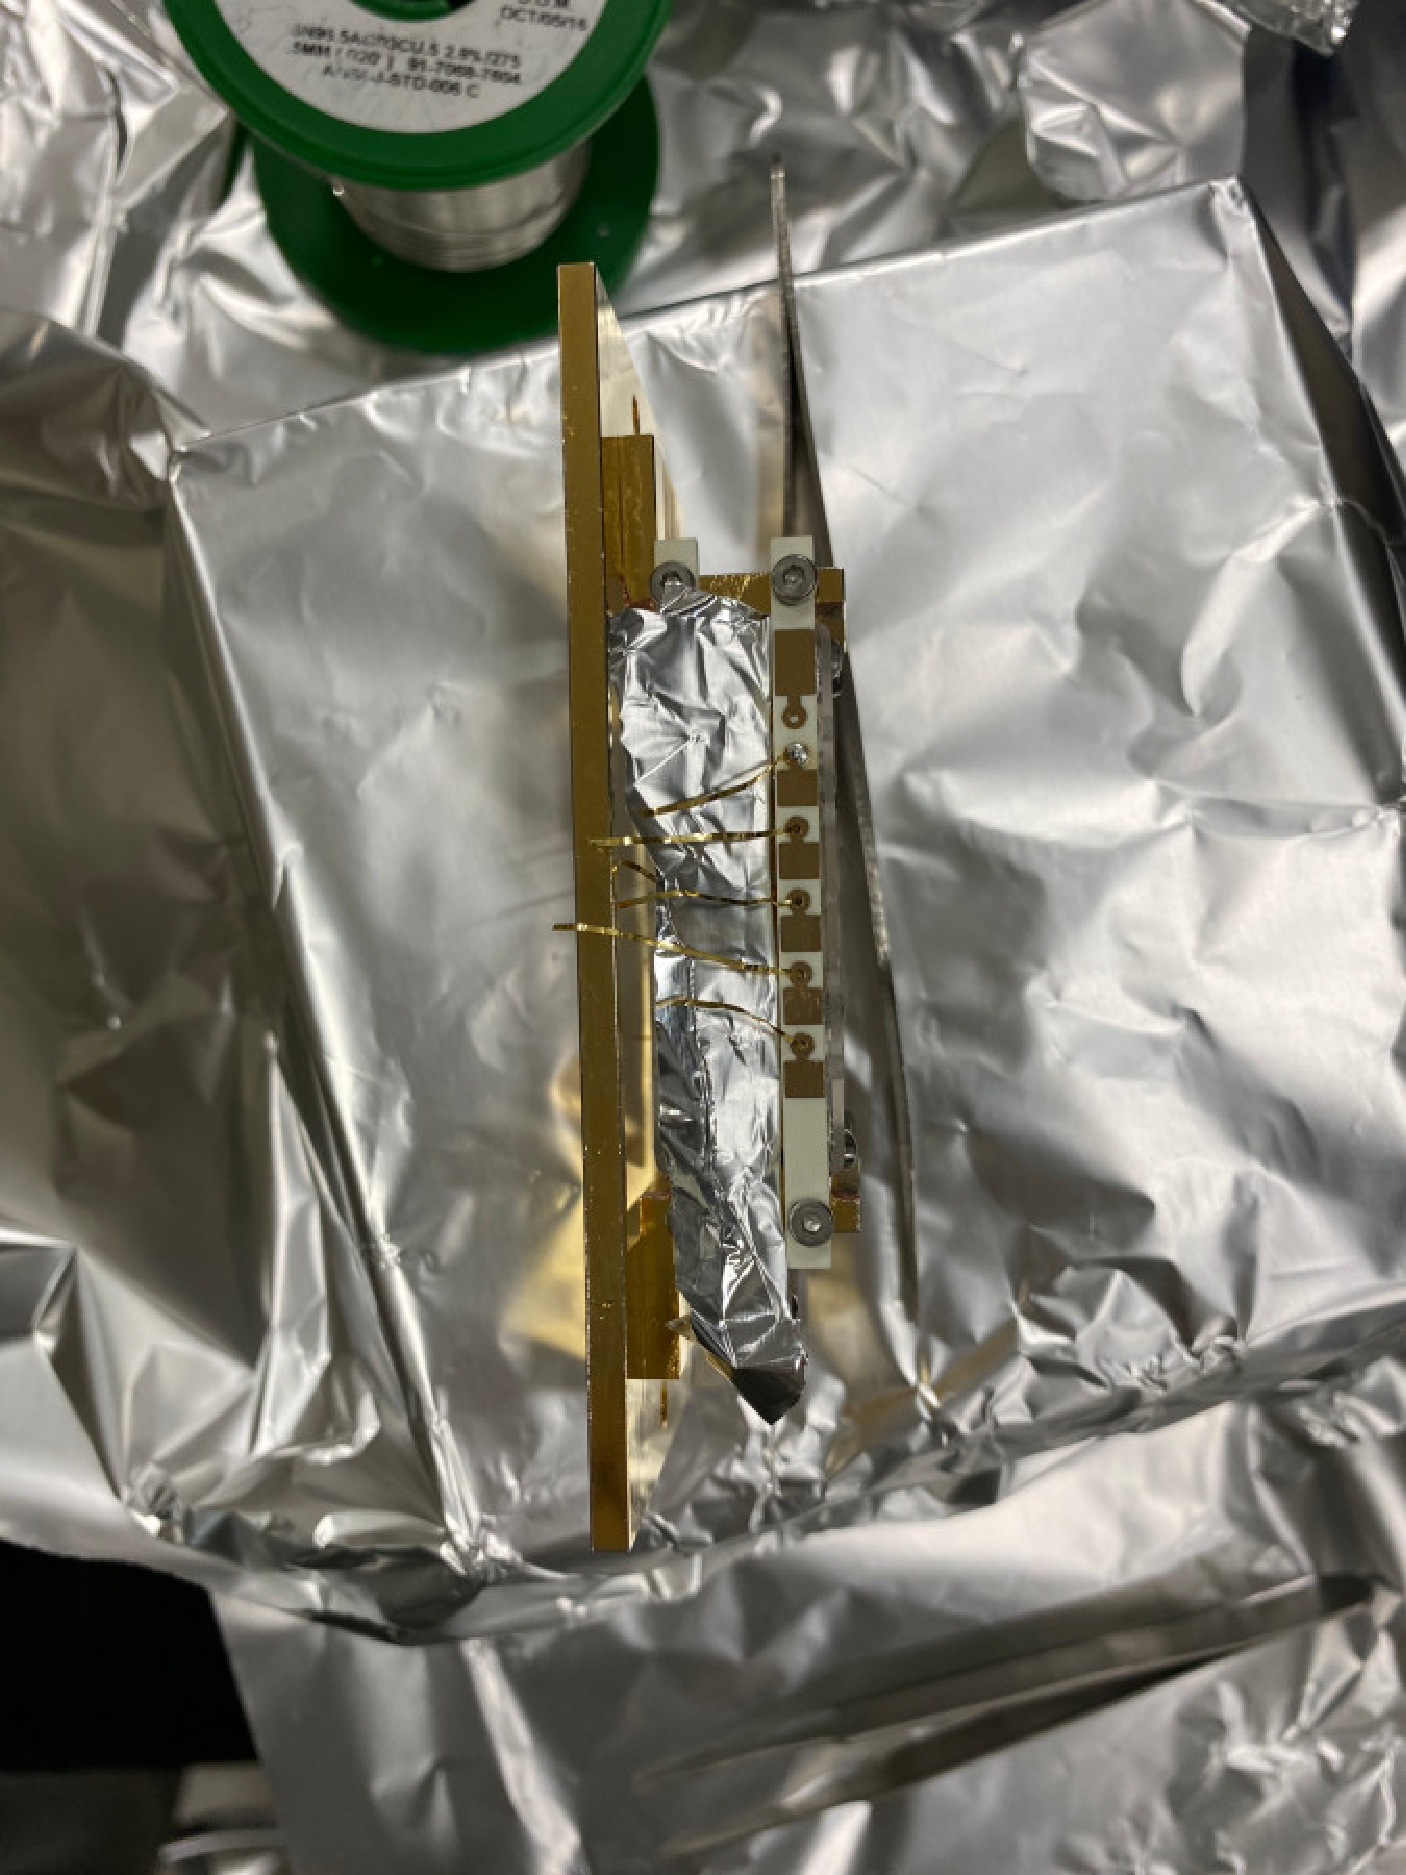
\includegraphics[width=0.4\linewidth]{fig_3_assembly_of_trap_pcb.pdf}}
    \caption{Assembly of the blade trap.}
\end{figure}

\begin{table}
    \centering
    \caption{Assembly procedures of the blade trap.}
    \begin{tabular}{p{0.2\linewidth}p{0.7\linewidth}}
        \toprule
        Procedure    & Content                                                                                                                                                                                                                                                                    \\

        \midrule
        Checking     & Soak the blades in acetone bath for 30 minutes, soak the blades in ethanol bath for 5 minutes, as the blades are very important and fragile.                                                                                                                               \\
                     & Process the DC 820pF capacitors, soak them in acetone bath for 5 minutes, soak them in ethanol bath for 1 minute.                                                                                                                                                          \\
                     & Lean the blades against the beaker, otherwise it is not easy to be taken out when it sinks.                                                                                                                                                                                \\
                     & The position of the DC capacitor is chosen to allow for clearance for the screws, as well as for the gold ribbon.                                                                                                                                                          \\
                     & The blades can be soaked in ethanol bath when not in use.                                                                                                                                                                                                                  \\
        Spot welding & Process the gold ribbon by sonicating it with acetone for 30 minutes and with ethanol for 5 minutes.                                                                                                                                                                       \\
                     & Cover the welding machine with aluminium foil before placing the blades to prevent them from scratching.                                                                                                                                                                   \\
        Preparation  & Prepare hlders, PCBs, sapphire chips, indium foil, M2 and M1.5 screw sets, spanners.                                                                                                                                                                                       \\
                     & Make indium foil soaked in acetone bath for 30 minutes and in ethanol bath for 5 minutes, sonicate the rest with acetone for 30 minutes and with ethanol for 5 minutes.                                                                                                    \\
        Assembly     & Apply indium foil to the sapphire piece, with the front of the indium foil flush with the top of the round hole to prevent short-circuiting the blade.                                                                                                                     \\
                     & Hold the blade parallel to the sapphire piece, remove the excess indium foil and fold the top of the gold ribbon                                                                                                                                                           \\
                     & Attach indium foil to the holder, then fix the sapphire piece to it, fix the PCB board to the side of the holder and pass the gold ribbon through the air, leaving a certain length of gold ribbon to prevent it from melting when soldering, donnot block the light path. \\
        \bottomrule
    \end{tabular}
\end{table}

The blade trap consists of four blade-shaped electrodes, one pair of DC electrodes and one pair of RF electrodes. The blade is processed by laser cutting the ceramic substrate and then plating the surface with a gold layer. The electrodes are machined with a certain amount of error and defects on the surface of the electrode closest to the ion produce a high level of electrical noise, which can be reduced by improving the process. We have machined a sapphire adapter plate and mounted the blade on the sapphire adapter plate and then mounted the sapphire adapter plate on an oxygen-free copper holder. We designed this adapter to avoid a short circuit between the blade and the ground (the blade holder). In order to increase the thermal conductivity, we need to cover these contact surfaces with indium foil. For the fixing of the components we used stainless steel screws and used resilient pads on each screw. This is to prevent the screws from loosening during the cooling down process, and to prevent the blade from being crushed by excessive torque when tightening the screws. Once installed we had to fine-tune the position of the sapphire adapter under the microscope to keep the assembly error small enough. This operation makes use of the fact that the diameter of the through-hole is slightly larger than the diameter of the screw. Since the assembly is done by hand, this part of the assembly error is unavoidable.

The connection of the blade electrodes is mainly done by means of gold ribbon (AMETEK) and Kapton insulated wire (Accu-Glass Products). When selecting materials we need to be aware of ultra-high vacuum and cryogenic compatibility. Some of the circuit connections are made prior to assembly and the rest is done afterwards. Before assembling the blade, a 820 pF capacitor is fixed with silver epoxy between each DC electrode and ground on the two DC blades. The purpose of this capacitor is to create a low impedance between the DC electrodes and ground, reducing the voltage splitting of the RF signal on the DC electrodes. The gold ribbon is connected to the electrodes with the spot welder at one end and to the pads of the PCB with solder at the other. We will later connect the pads to the corresponding connections with Kapton insulated wire, where the DC electrode wires are connected to the corresponding wires from the DC feedthrough through the heat sink twice, and the two RF electrode wires are connected to the two wires at the output of the helical resonator.



\section{Yb oven}

In order to generate the atomic beams of Yb, we built two separate ovens from two stainless steel tubes, but integrated into a single feedthrough and both able to be used to load ions. The ${ }^{171} \mathrm{Yb}$ oven has an abundance of 90\% and The ${ }^{174} \mathrm{Yb}$ oven has an abundance of 98\%. As the Yb source is in block form, we need to cut it into small pieces and insert it into the stainless steel tube.

\begin{figure}
    \centering
    \subcaptionbox{Put all the components together.}
    {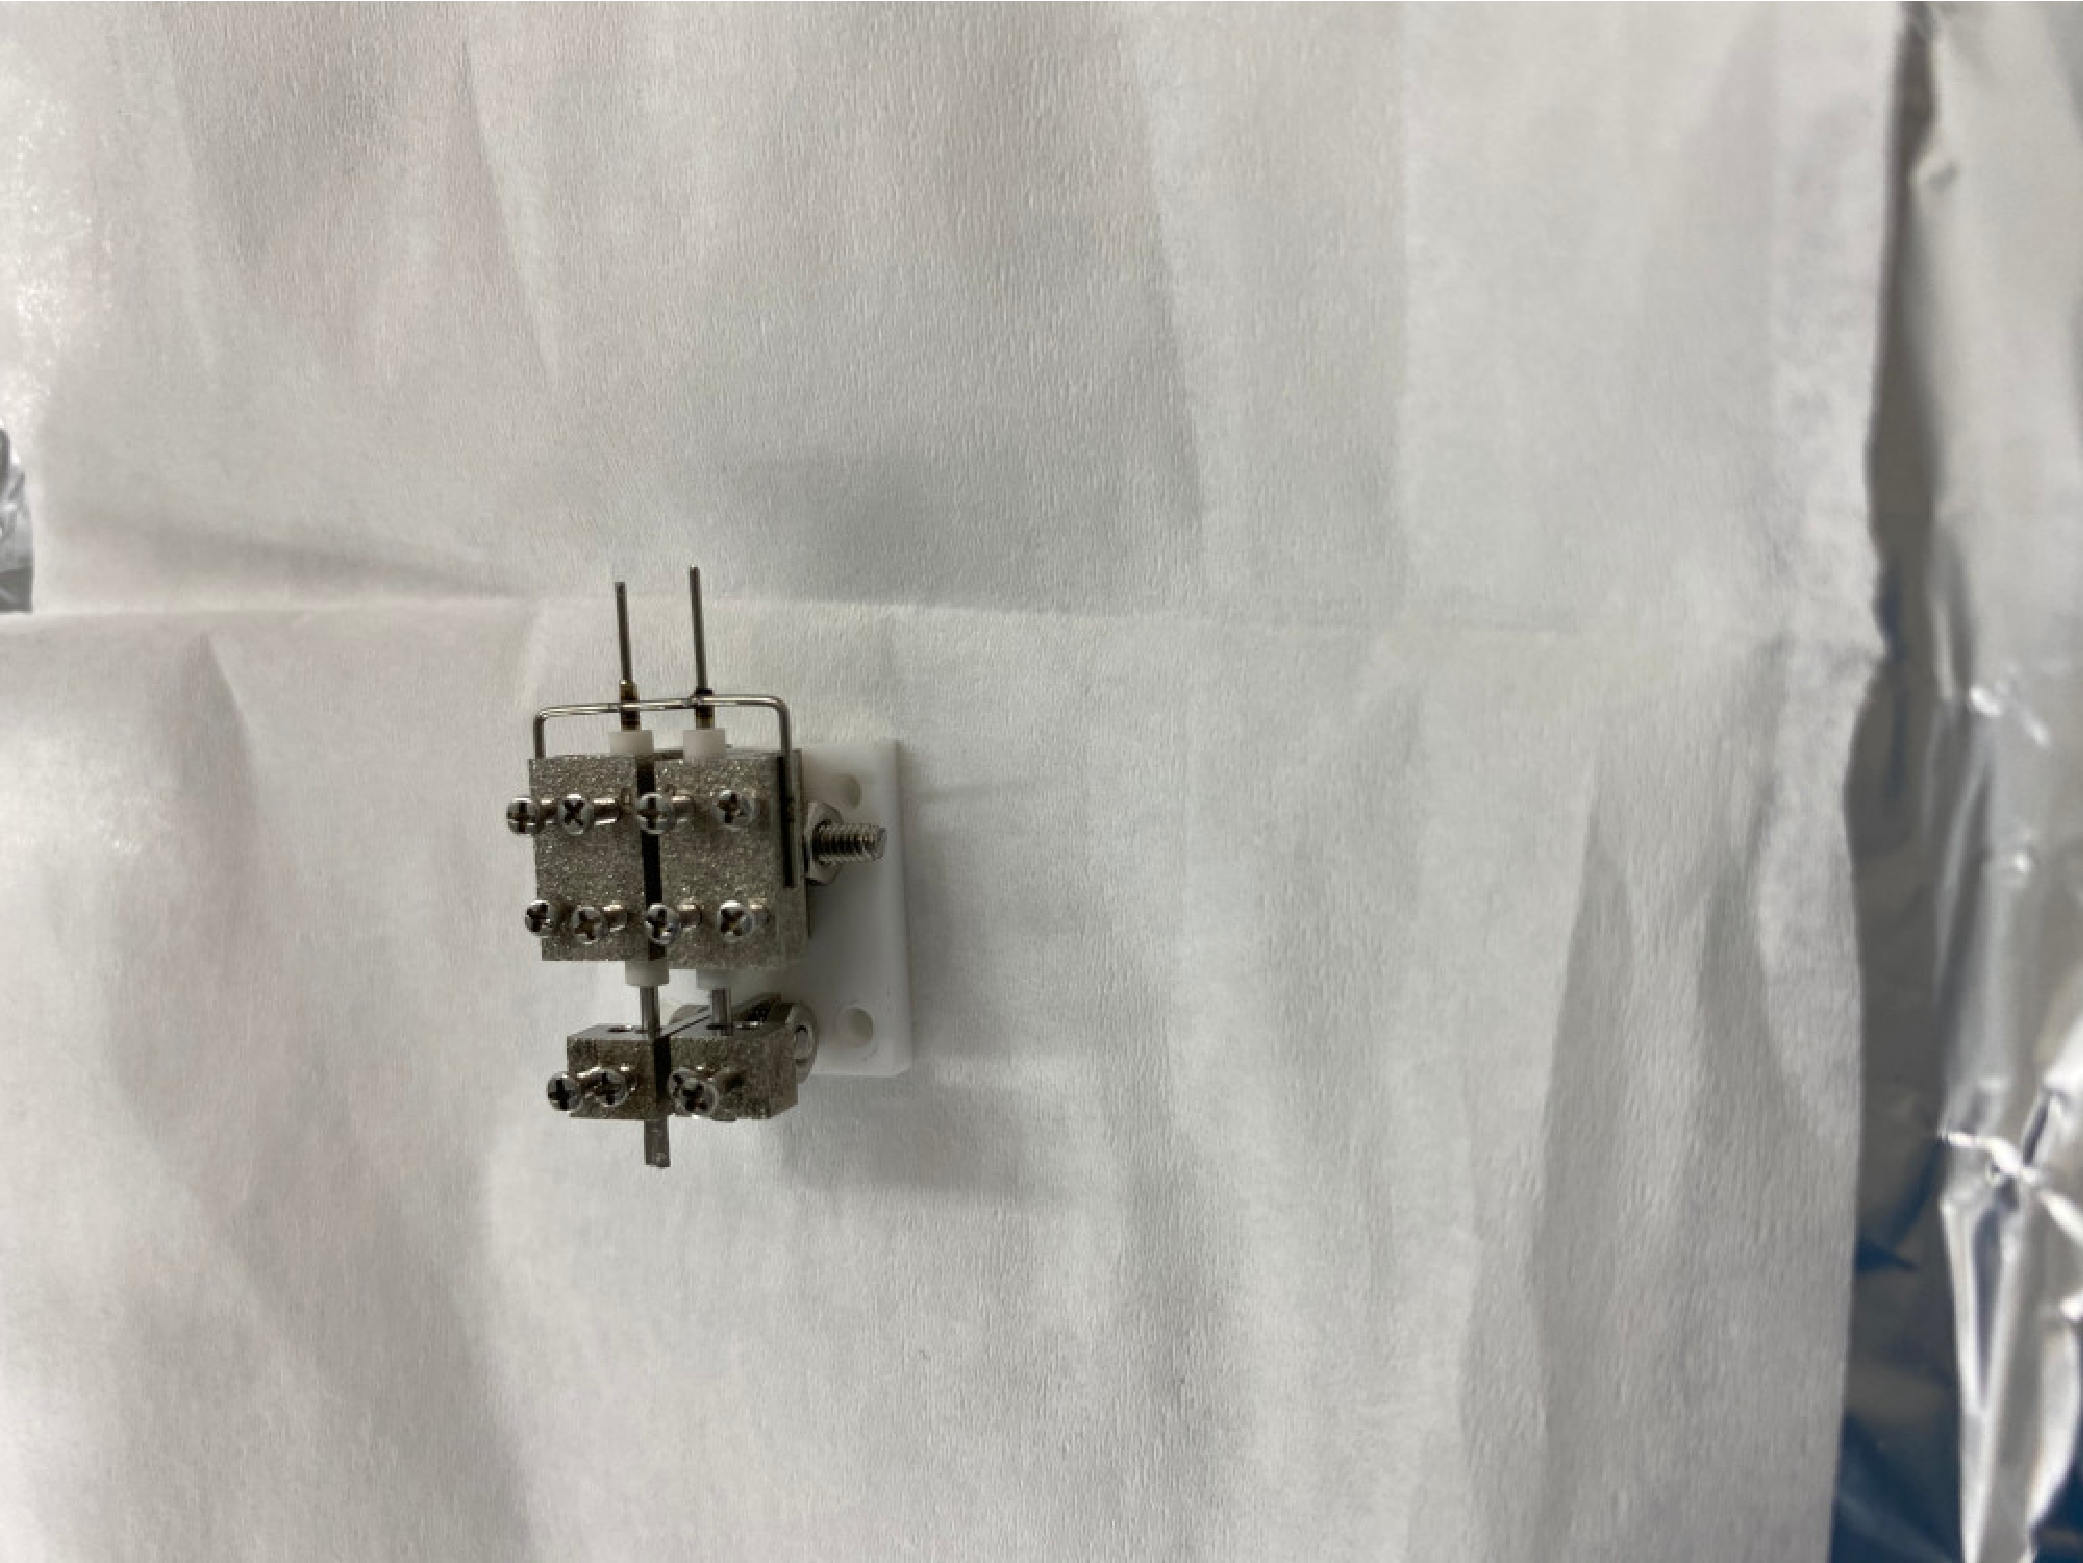
\includegraphics[width=0.4\linewidth]{fig_3_assembly_of_oven_1.pdf}}
    \subcaptionbox{Connect to feedthrough.}
    {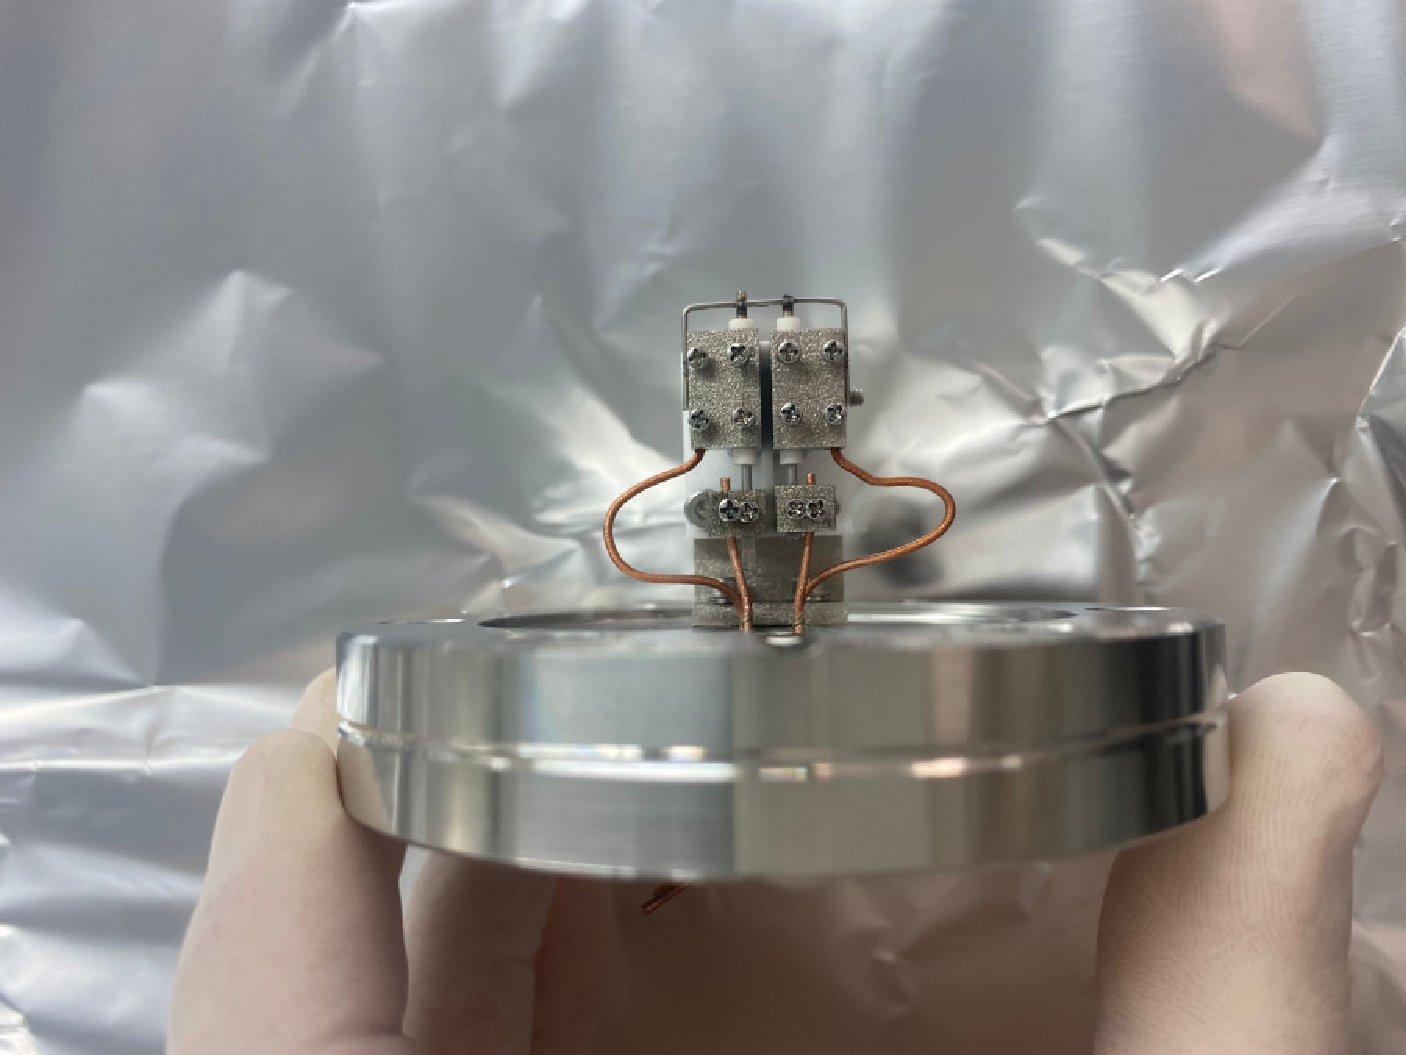
\includegraphics[width=0.4\linewidth]{fig_3_assembly_of_oven_2.pdf}}
    \caption{Assembly of the Yb oven.}
\end{figure}

In order to achieve UHV compatibility we chose to use copper, stainless steel and Macor when machining the parts of the oven. Before assembly and testing, we cleaned all the parts inside the ultrasound machine using acetone and ethanol as solvents. All the parts were assembled according to the drawings and the copper wires on the feedthrough were attached to the stainless steel base, which was all screwed in place. We then used a spot welder and welded the stainless steel tube to the stainless steel wire, and the stainless steel wire to the stainless steel base, respectively. As the stainless steel tube has the smallest cross-sectional area, the highest resistance in the whole circuit is at the stainless steel tube, about 0.5 $\Omega$, so the temperature is highest here too. I would recommend having some extra spare parts and testing the parameters of the spot welder in advance, as the stainless steel tube can easily break under unsuitable parameters. Finally the two Yb sources are filled into the corresponding stainless steel tubes.

\begin{figure}
    \centering
    \subcaptionbox{Testing in a vacuum.}
    {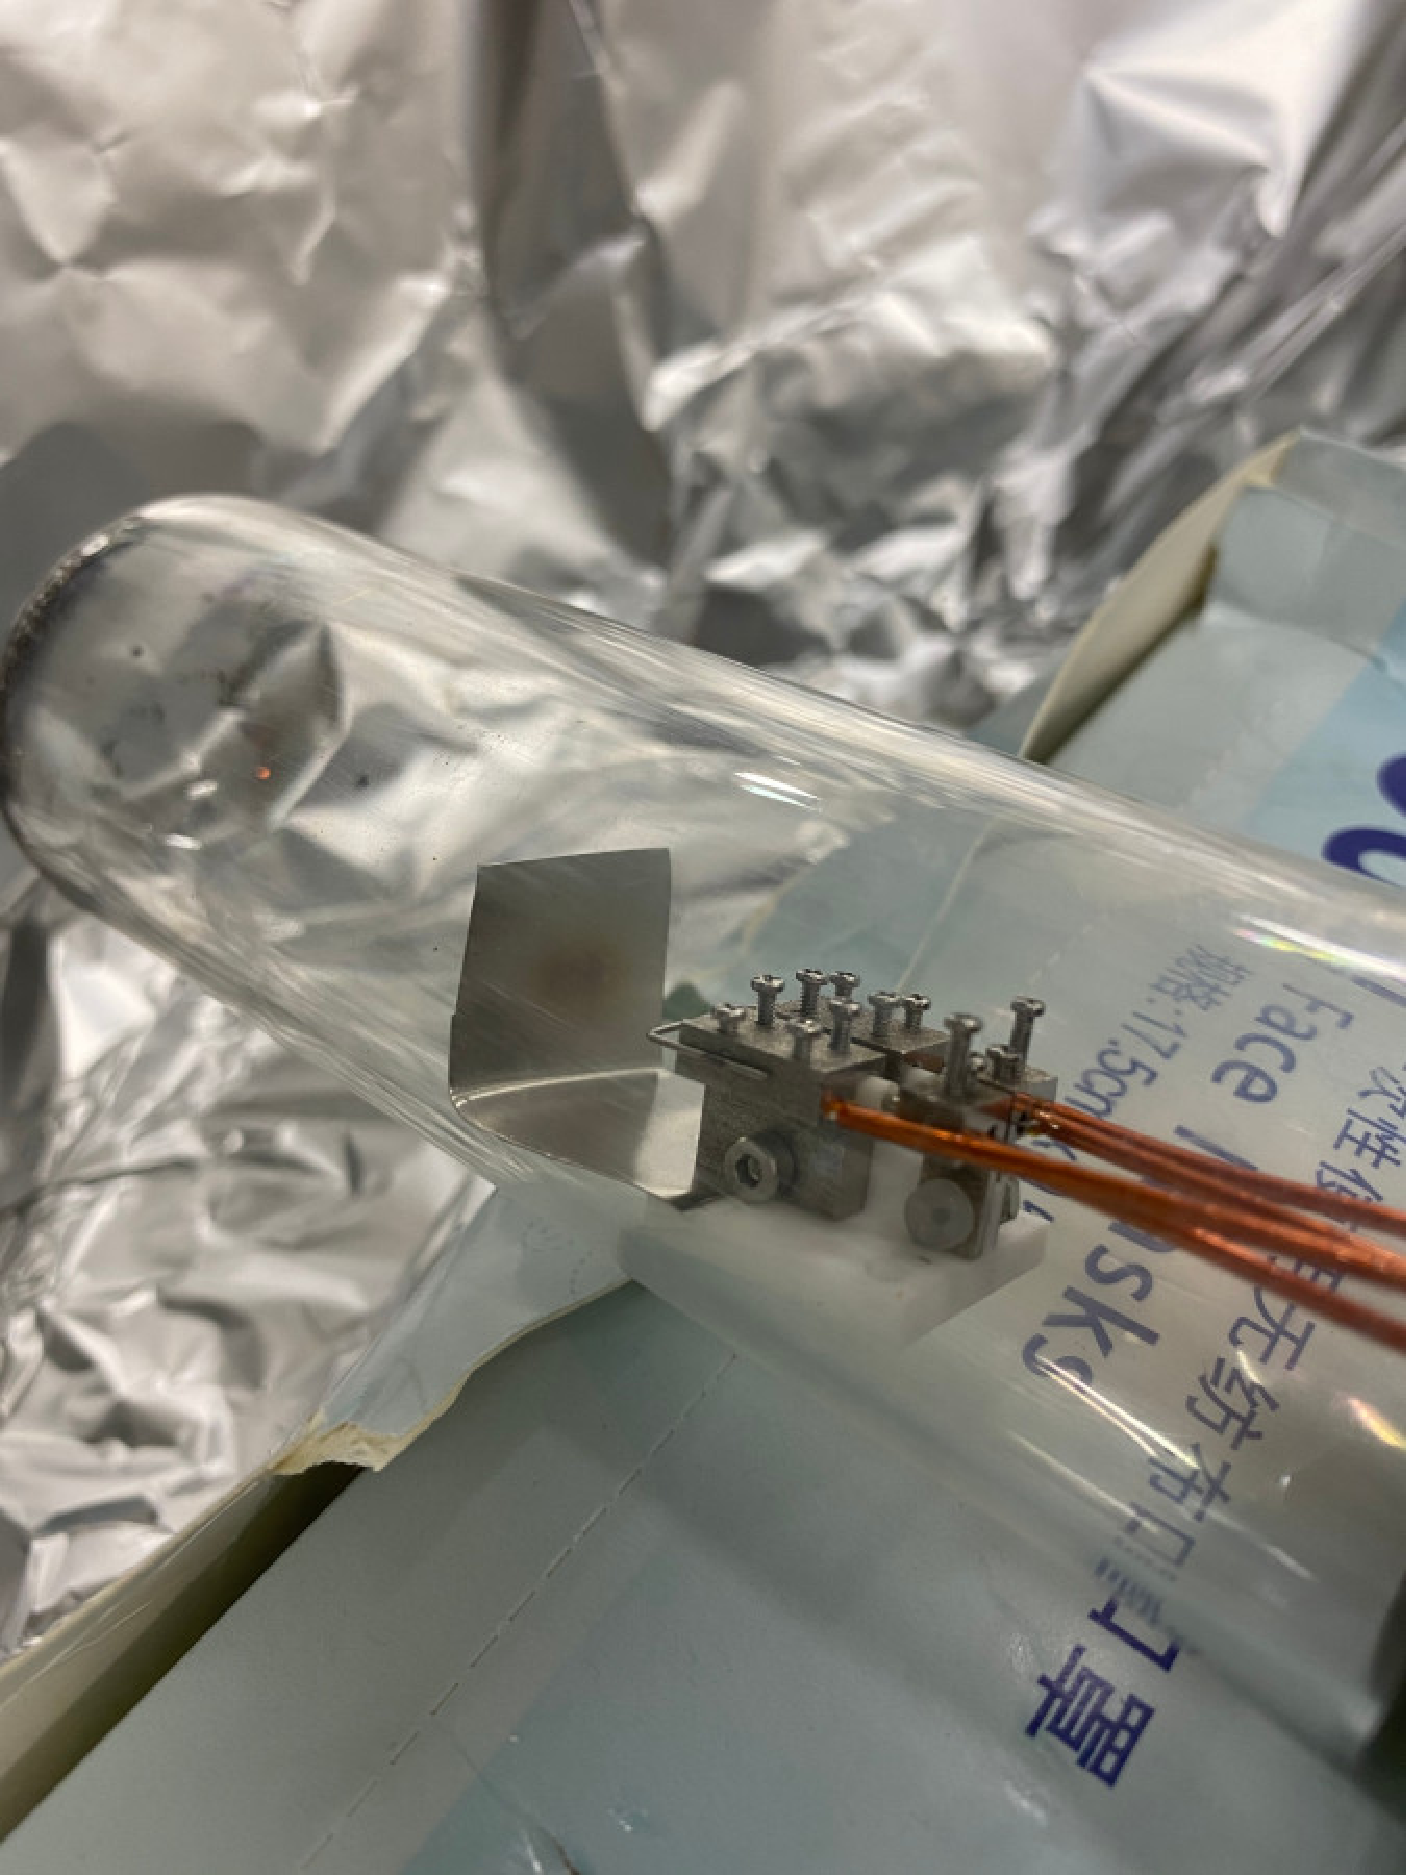
\includegraphics[width=0.3\linewidth]{fig_3_test_oven_1.pdf}}
    \subcaptionbox{Observation in the atmosphere.}
    {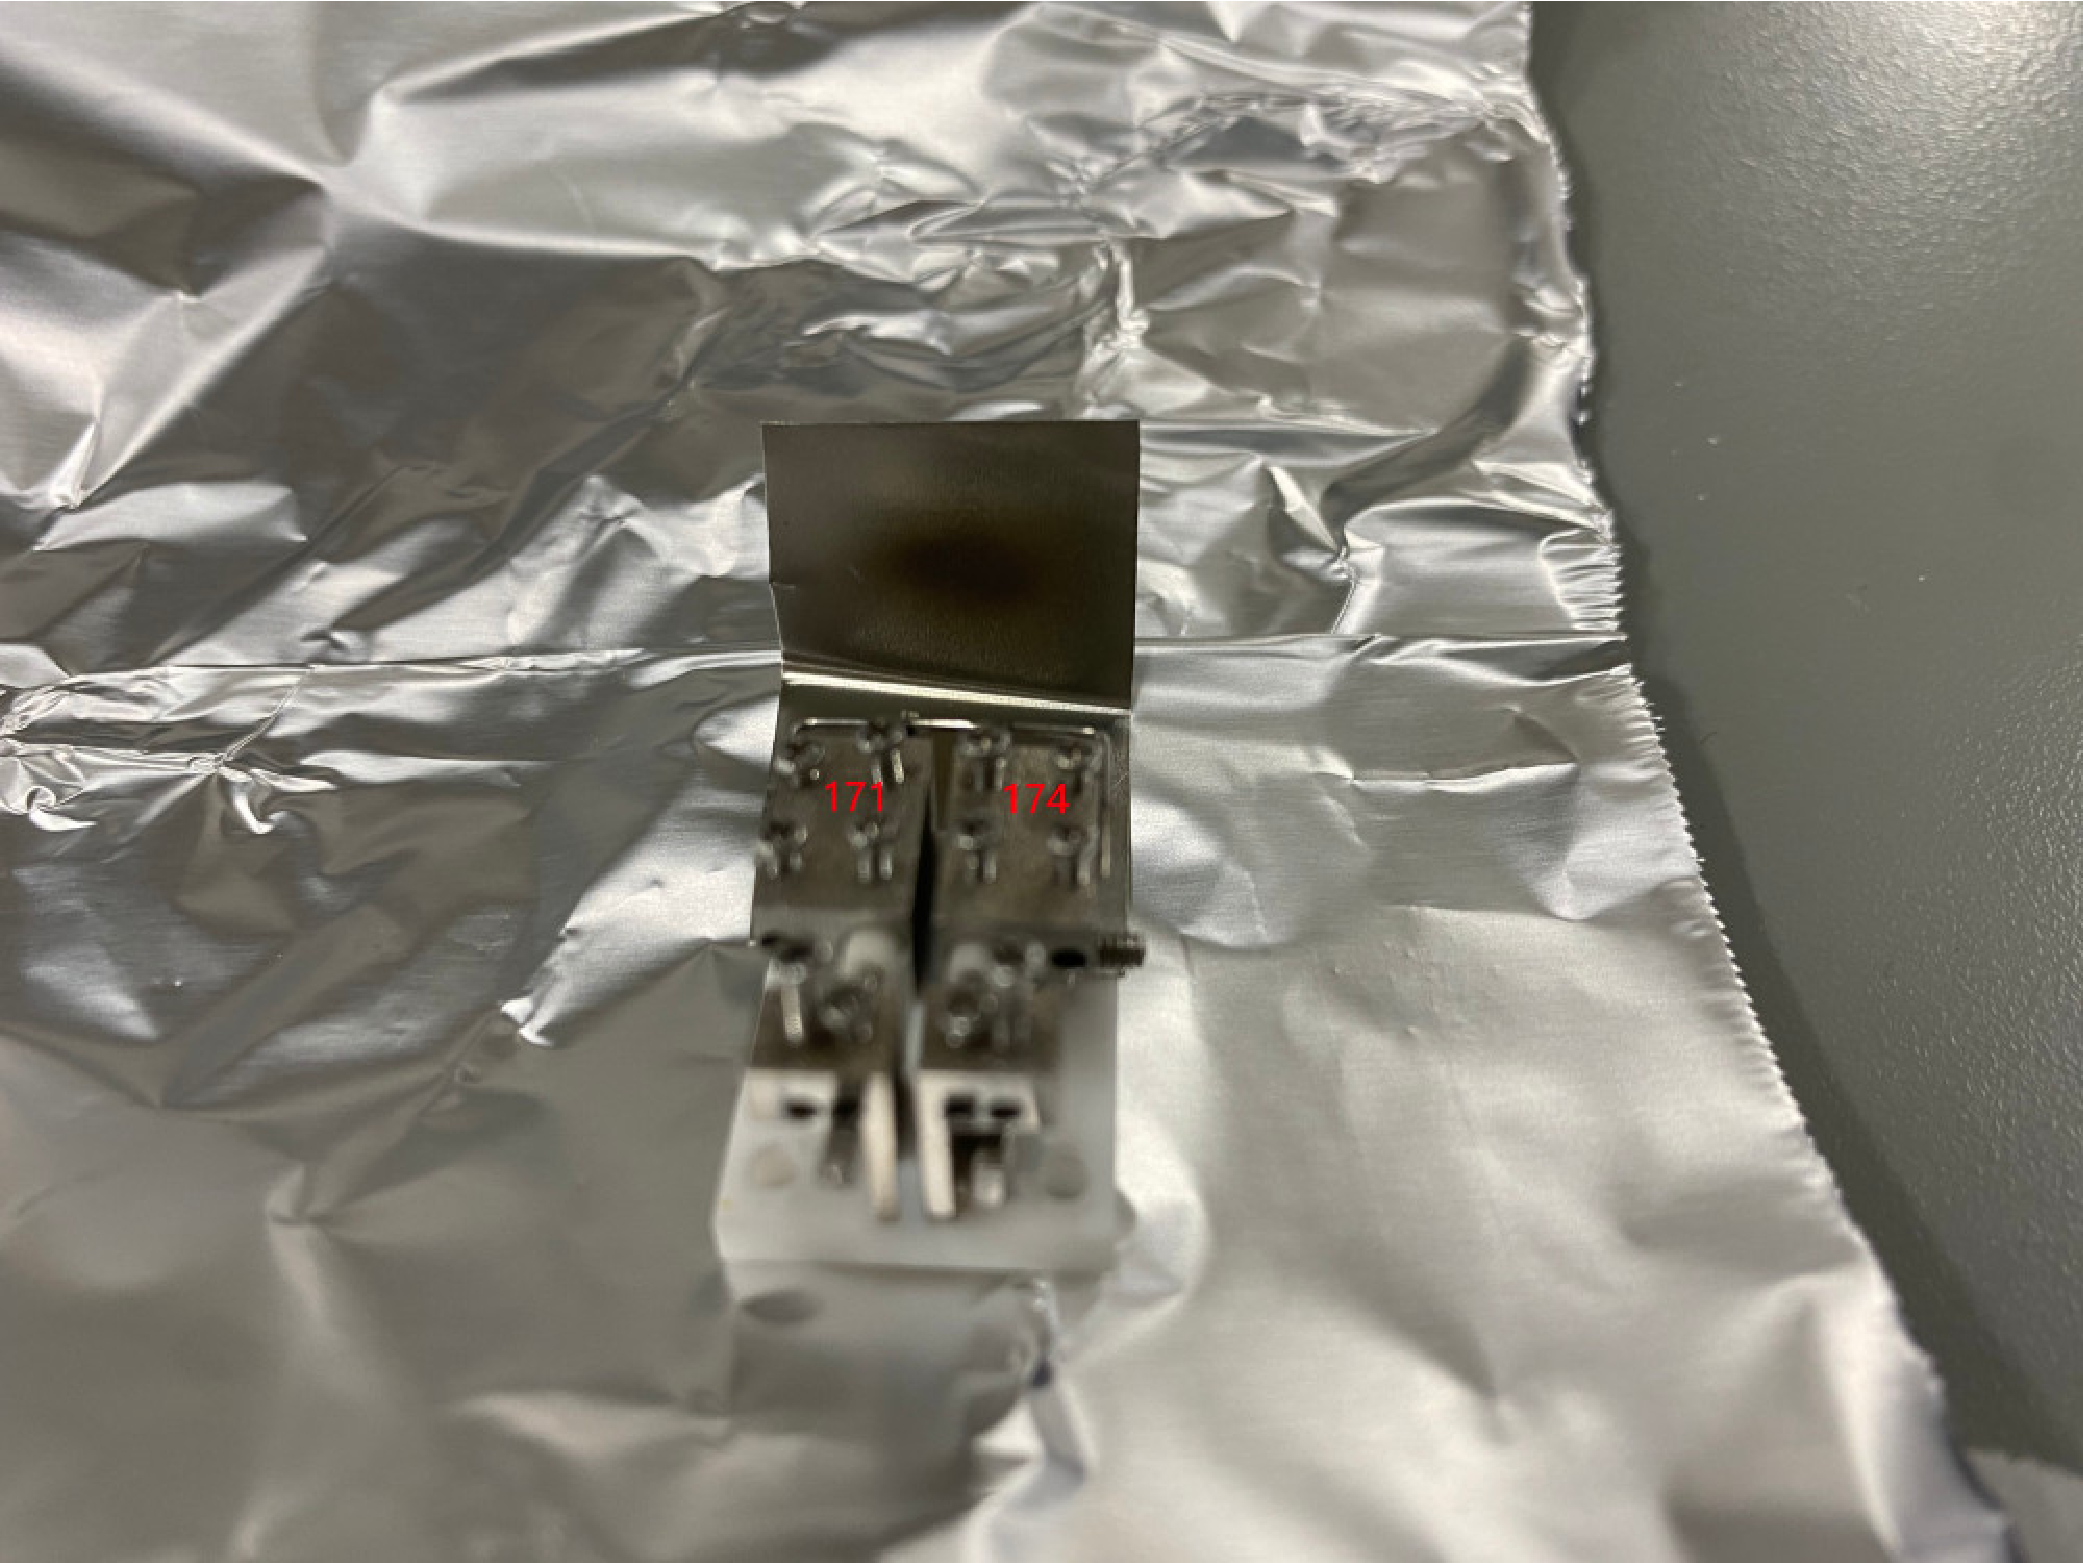
\includegraphics[width=0.5\linewidth]{fig_3_test_oven_2.pdf}}
    \caption{Testing of the Yb oven.}
\end{figure}

Each oven is mounted in such a way that the outgoing atomic beam is directed towards the trapping area. The oven feedthrough replaces an 1 inch window in the axial direction of the trap. the glass in the corresponding position of the 40 K shield and 4 K shield is also replaced with a round aluminium plate, the centre of which is a square hole with a 5mm side to pass through the Yb flux. As the cryostat has assembly errors, I would recommend preparing round aluminium plates with different opening positions in advance. Ultimately we need to be able to see the trap through the opposite window, with the square hole and the oven in the same line.

\begin{table}
    \centering
    \caption{Parameter variation during Testing the Yb oven.}
    \begin{tabular}{llll}
        \toprule
        Oven                            & Initial vacuum              & Ending vacuum               & Threshold current \\

        \midrule
        ${ }^{171} \mathrm{Yb}$ (Left)  & $4.0 \times {10}^{-6}$ mbar & $8.6 \times {10}^{-6}$ mbar & 4.2 A             \\
        ${ }^{174} \mathrm{Yb}$ (Right) & $2.3 \times {10}^{-6}$ mbar & $6.5 \times {10}^{-6}$ mbar & 3.9 A             \\
        \bottomrule
    \end{tabular}
\end{table}


In the process of loading ions, when this stainless steel tube is heated resistively by an electric current, a spray of atomic Yb is produced. The temperature reached depends on the current and the time of operation. If either of these two factors is too high or too long, this can lead to rapid evaporation of the Yb and thus the formation of a spray dense enough to cover its surface (e.g. ion trap electrodes or vacuum windows). To prevent this, each oven is tested in advance. A stainless steel sheet is placed in front of the oven and then the oven is placed in a transparent vacuum chamber and the vacuum is reduced to approximately $4 \times {10}^{-6}$ mbar using a turbo-molecular pump, so that a test system can be set up. We tested each oven in turn, starting at 0 A and increasing the current by 0.1 A every 10 seconds, observing the change in vacuum level and the colour of the stainless steel sheet. We can observe both the darkening of the stainless steel sheet and the rapid rise in pressure, at which point the current value is the threshold current for the corresponding oven. ${ }^{171} \mathrm{Yb}$ oven has a threshold current of 4.2 A and ${ }^{174} \mathrm{Yb}$ oven has a threshold current of 3.9A, but the current values we use in practice will be lower than this threshold, the exact values need to be measured in the corresponding experiments. The exact values need to be measured in corresponding experiments, such as observing the fluorescence of Yb atoms and loading Yb ion.



\section{Optical and imaging system}

\begin{figure}
    \centering
    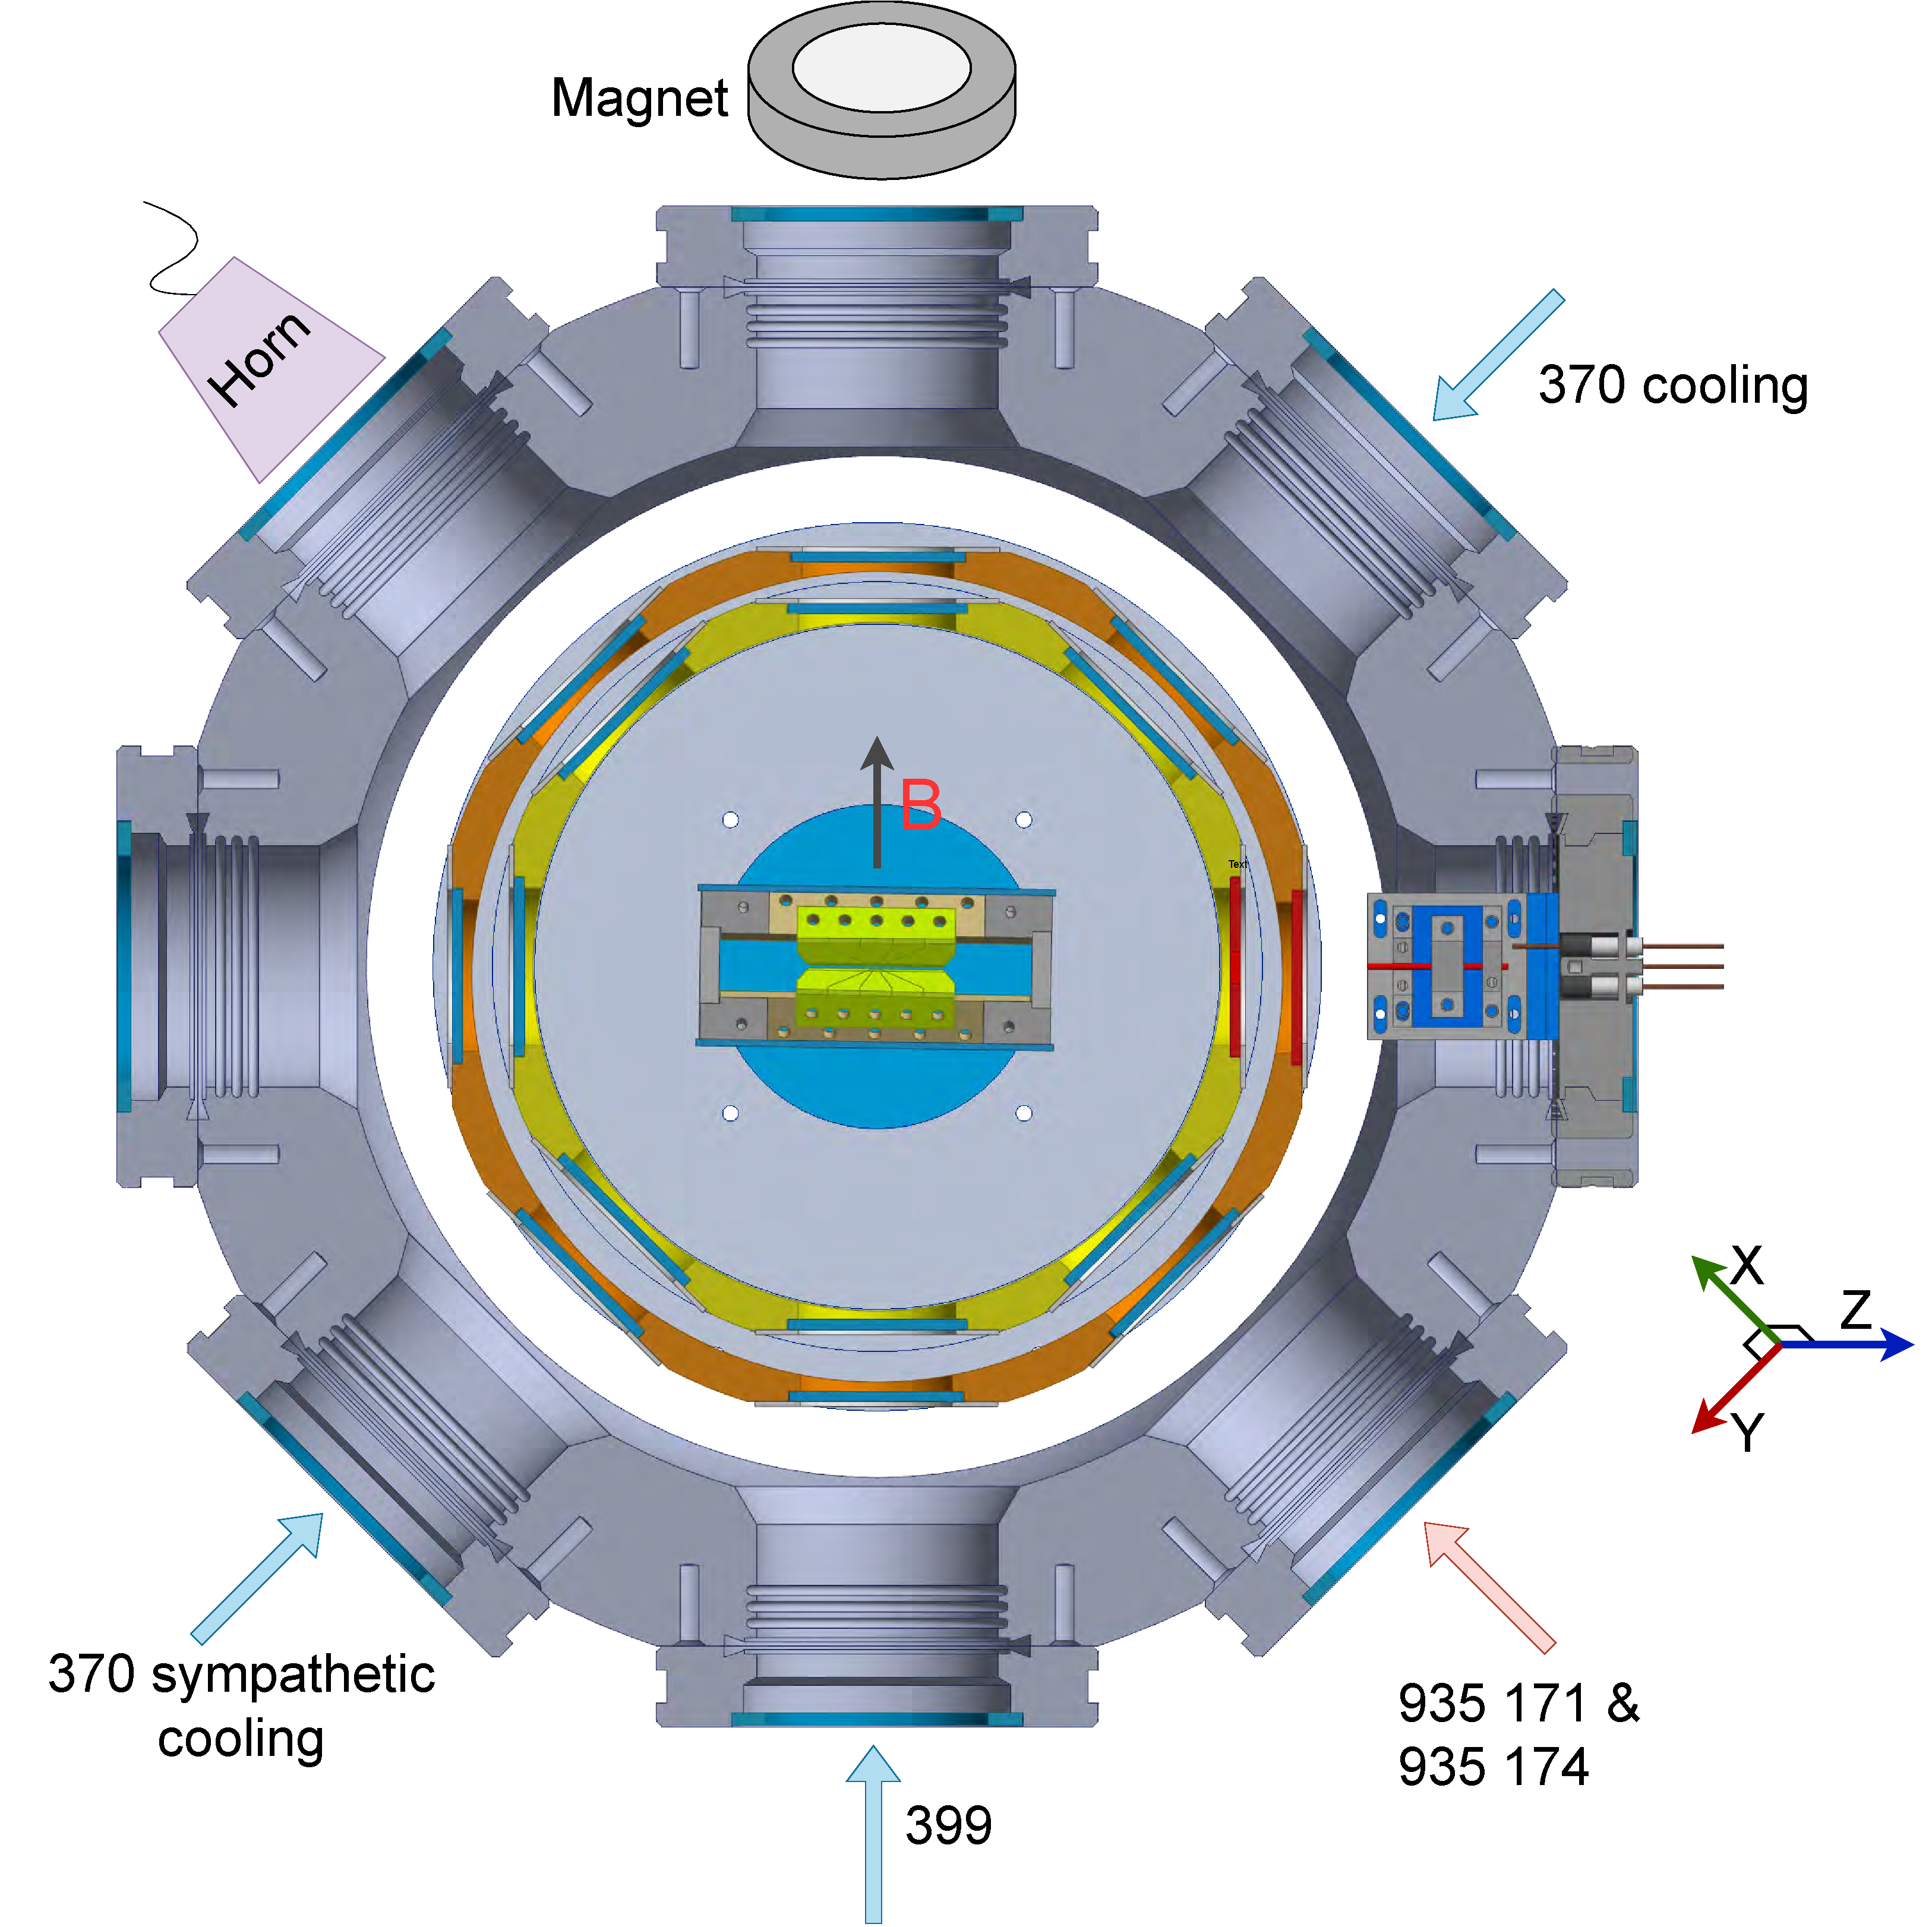
\includegraphics[width=0.7\linewidth]{fig_3_optical_layout_of_ion_trap_and_vacuum_chamber.pdf}
    \caption{Optical layout of the ion trap and the vacuum chamber.}
\end{figure}

Whether trapping ions or manipulating them, we need lasers. In our laboratory, tunable diode lasers (Toptica DL pro HP) are used widely, mainly because these products are very well mature. For ion trap systems, a stable light source is very important. Experimentally, we need these lasers to be switched on and off quickly, typically in a few hundred nanoseconds. It is also necessary that these lasers can be stabilised over long periods of time and that these laser controllers have stable software systems. Laser stabilisation covers mode, frequency, power and polarisation. Typical laser stabilisation lasts from a few hours to a day, including laser frequency locking. This is sufficient for our trapped ion experiments, but longer stabilisation times are preferable. In the experiments, these stable lasers are used for: ion loading, Doppler cooling, optical pumping, state detection, repumping and sympathetic cooling. In addition to the laser light path into the cavity, I also built an imaging system to collect the fluorescence emitted by the ions, enabling real-time observation and state detection of the ions.

\subsection{Laser sources and power allocation}

The light sources in the laboratory are placed on several separate optical tables. Since the principles of the optical path setup are similar, we can present the light sources and power allocation in a common way, as shown in Fig~\ref{fig:fig_3_optical_path_diode_laser}. The cryogenic trap platform requires a 370 nm laser (L1), a 399 nm laser (L2) and two 935 nm lasers (L3, L4). The two 935 nm lasers are shared with other ion trap platforms in the lab, one for trapping ${ }^{171} \mathrm{Yb}^{+}$ ions and the other for trapping ${ }^{174} \mathrm{Yb}^{+}$ ions. The 399 nm laser is used for loading ions. Depending on the type of ion to be loaded, ${ }^{171} \mathrm{Yb}^{+}$ or ${ }^{174} \mathrm{Yb}^{+}$, we can change the wavelength of the 399 nm laser. This 399 nm laser is also shared with other trapped ion platforms in the lab and only one 399 nm laser is needed. Since loading ions is not very frequent and most of the time we need to load ${ }^{171} \mathrm{Yb}^{+}$ ions, and modifying the wavelength of the 399 nm laser will not affect the stable trapping of the loaded ions.

\begin{figure}
    \centering
    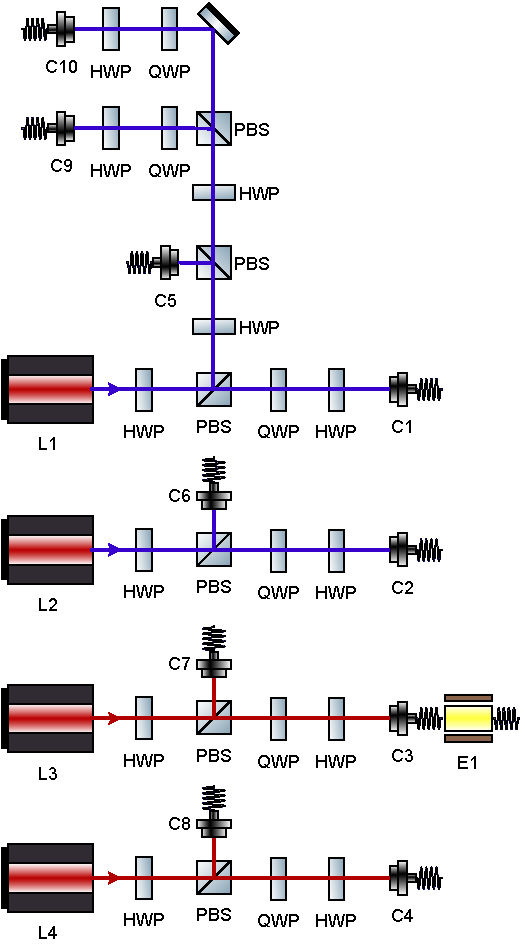
\includegraphics[width=0.4\linewidth]{fig_3_optical_path_diode_laser.pdf}
    \caption{Optical path of laser power allocation.}
    \label{fig:fig_3_optical_path_diode_laser}
\end{figure}

The output power of a semiconductor laser is approximately 10 mW, depending on the wavelength and model, the laser output power may vary a little. The output power of the 370 nm laser (L1) is 13 mW,
other lasers have similar output power.

As the nominal light output from the laser is linearly polarised, a power attenuation unit was formed using a half-wave plate(HWP) and polarization beam splitter(PBS )to split the laser output into two parts, which are separately coupled into the fibre. Each fibre will act as the light source for the next stage of the optical path, thus making the optical path a modular one. Each laser has one optical fibre connected to the wavemeter (C5, C6, C7, C8). Because polarisation stabilisation is not required, a single-mode fibre is used, with a typical power of approximately 50 µW. The other fibres are the light sources for the rear optical paths (C1, C2, C3, C4) and require high power, typically 5 mW. At the same time their polarisation needs to be stable over time and we use single-mode polarization-maintaining fibres. In order to adjust the polarisation direction to match that of the single-mode polarisation-maintaining fibre, we use a polarisation adjustment unit consisting of a HWP and quarter-wave plate(QWP). We need to maximize the efficiency of the fiber coupling, which requires a good laser output mode and good mode matching, which can be done with a lens pair, I don't show this in the diagram.

\begin{table}
    \centering
    \caption{Wavelengths of lasers in the laboratory corresponding to loading different isotopes.}
    \begin{tabular}{llll}
        \toprule
        Isotope                     & 370 Laser (nm) & 399 Laser (nm) & 935 Laser (nm) \\
        \midrule
        ${ }^{171} \mathrm{Yb}^{+}$ & 369.526334     & 398.911150     & 935.188        \\
        ${ }^{174} \mathrm{Yb}^{+}$ & 369.525228     & 398.911570     & 935.180        \\
        \bottomrule
    \end{tabular}
\end{table}

The 370 nm laser also has two splits: one (C9) is connected to the optical cavity for narrow linewidth frequency locking of the laser, and the other (C10) is set aside. ${ }^{171} \mathrm{Yb}^{+}$ repumping beam requires 3.0695 GHz sidebands, so the 935 nm laser (L3) has a fibre EOM (E1) in the rear optical path.

\subsection{Laser frequency stabilization}

\begin{figure}
    \centering
    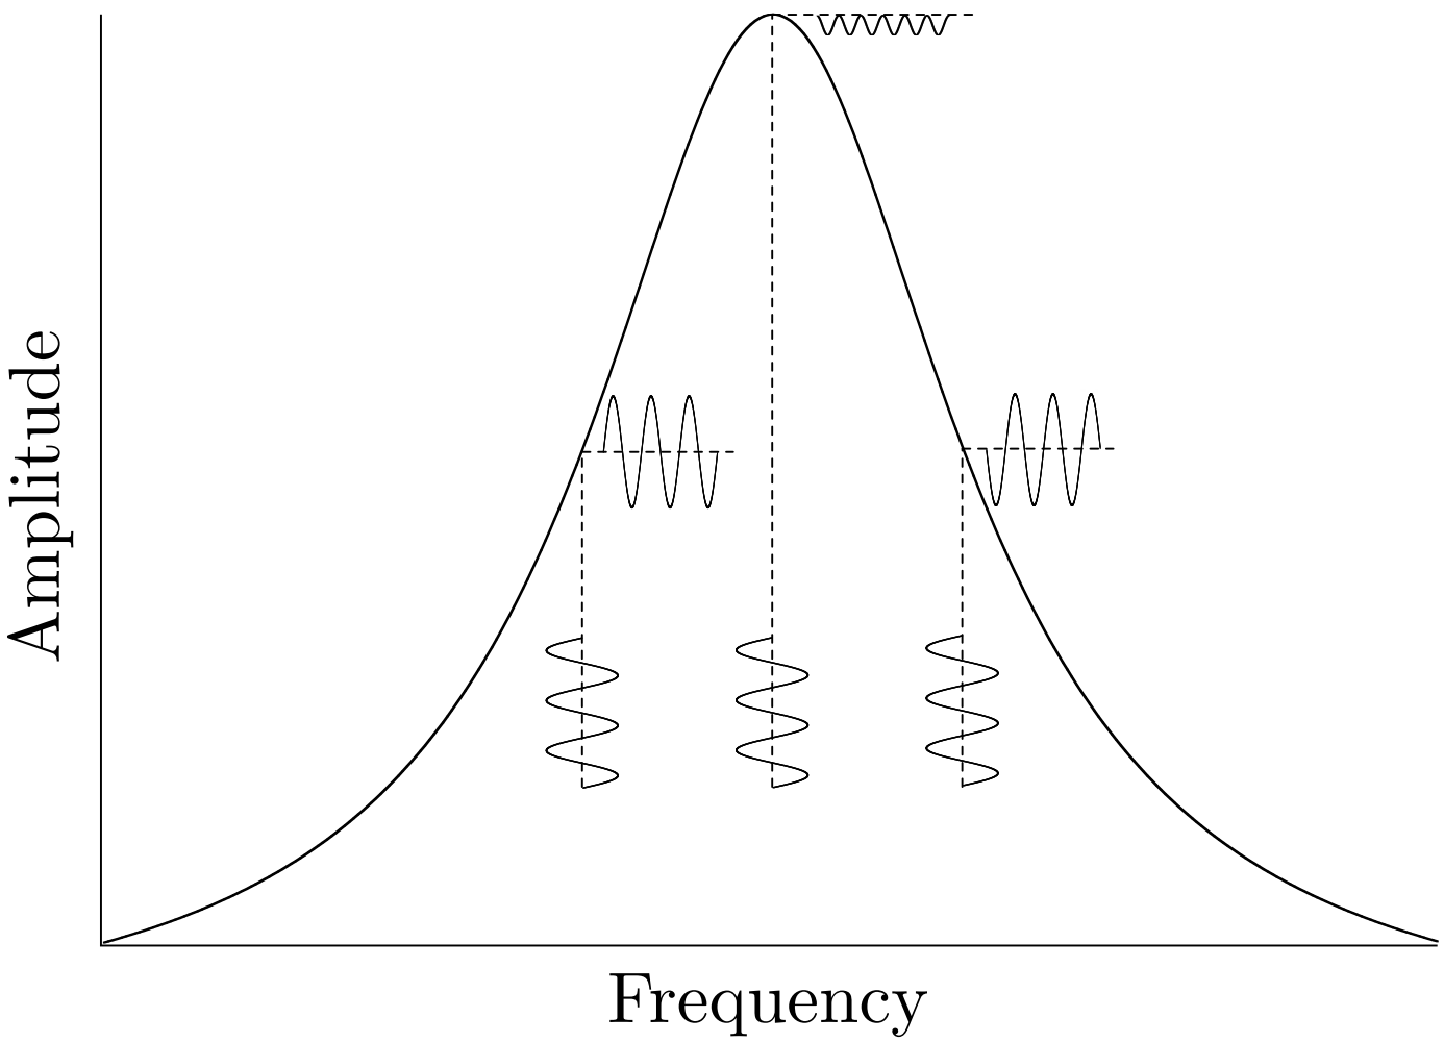
\includegraphics[width=0.4\linewidth]{fig_3_principle_of_frequency_modulation_for_optical_cavity.pdf}
    \caption{Illustration of simple frequency modulation for optical cavity.}
\end{figure}

The target linewidth of the laser frequency locking determines the laser frequency locking scheme. In my experiments there is no need for ultra-narrow linewidth laser locking, so the laser locking scheme is relatively simple and I have mainly optimised the automatic control of the frequency locking process. The measurement and locking of the laser frequency can be achieved with a wavelength meter, which has a relatively low bandwidth of about 10 Hz because the sum of the measurement time of the multi-channel wavelength meter and the computer readout time is about 100 ms, as shown in Fig~\ref{fig:fig_3_optical_path_wave_meter}. The standard deviation of the output frequency of the laser locked with this scheme is about 1 MHz, which meets my needs with a 399 nm laser and two 935 nm lasers, or if only to trap a small amount of ions then also my requirements for a 370 nm laser. The outgoing light from the laser is transmitted by optical fibres (C5, C6, C7, C8) to the input of the wavemeter, which is programmed to read the frequency on our PC and then programmed to adjust the voltage signal from the laser controller, thus creating a closed loop that locks the laser frequency. The wavemeter's measurements are affected by the environment, mainly air pressure and temperature. Therefore this frequency locking scheme will cause the locked laser frequency to be inaccurate due to inaccurate measurements, but this error is slow and periodic over time. So for 399 nm laser and 935 nm lasers we don't take this into account. I only calibrate the 370 nm laser once in 1 hour or longer, by measuring the resonant frequency of the $\mathrm{Yb}^{+}$ ion and feeding it back to the wavemeter's lock point. It would be possible to automatically calibrate the wavemeter for measurement errors if the wavemeter had a locked reference light all the way through, such as a 780 nm laser, but we have not done this because it is not necessary. The implementation of an automatic frequency lock is necessary as it will simplify the steps of daily operation. By laboratory standards these lasers need to be switched off when they are not in use, for example every night. I will adjust the operating parameters of the laser so that the laser mode can be stabilised back to a specific frequency range for approximately 10 minutes after each switch-on operation, which requires us to find a stable operating parameter for the laser. We then only need to program to communicate with the laser and the wavemeter to achieve automatic laser control and frequency locking.

\begin{figure}
    \centering
    \subcaptionbox{Optical path of the wavelength meter.\label{fig:fig_3_optical_path_wave_meter}}
    {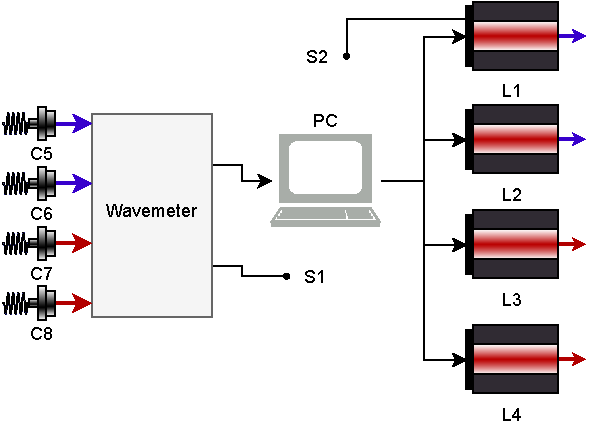
\includegraphics[width=0.4\linewidth]{fig_3_optical_path_wave_meter.pdf}}
    \subcaptionbox{Optical path of the optical cavity.\label{fig:fig_3_optical_path_370_cavity}}
    {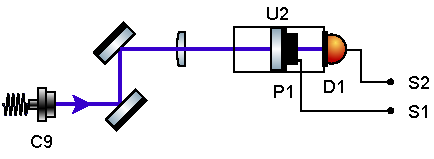
\includegraphics[width=0.4\linewidth]{fig_3_optical_path_370_cavity.pdf}}
    \caption{Optical layout of laser frequency stabilization system.}
\end{figure}

\begin{figure}
    \centering
    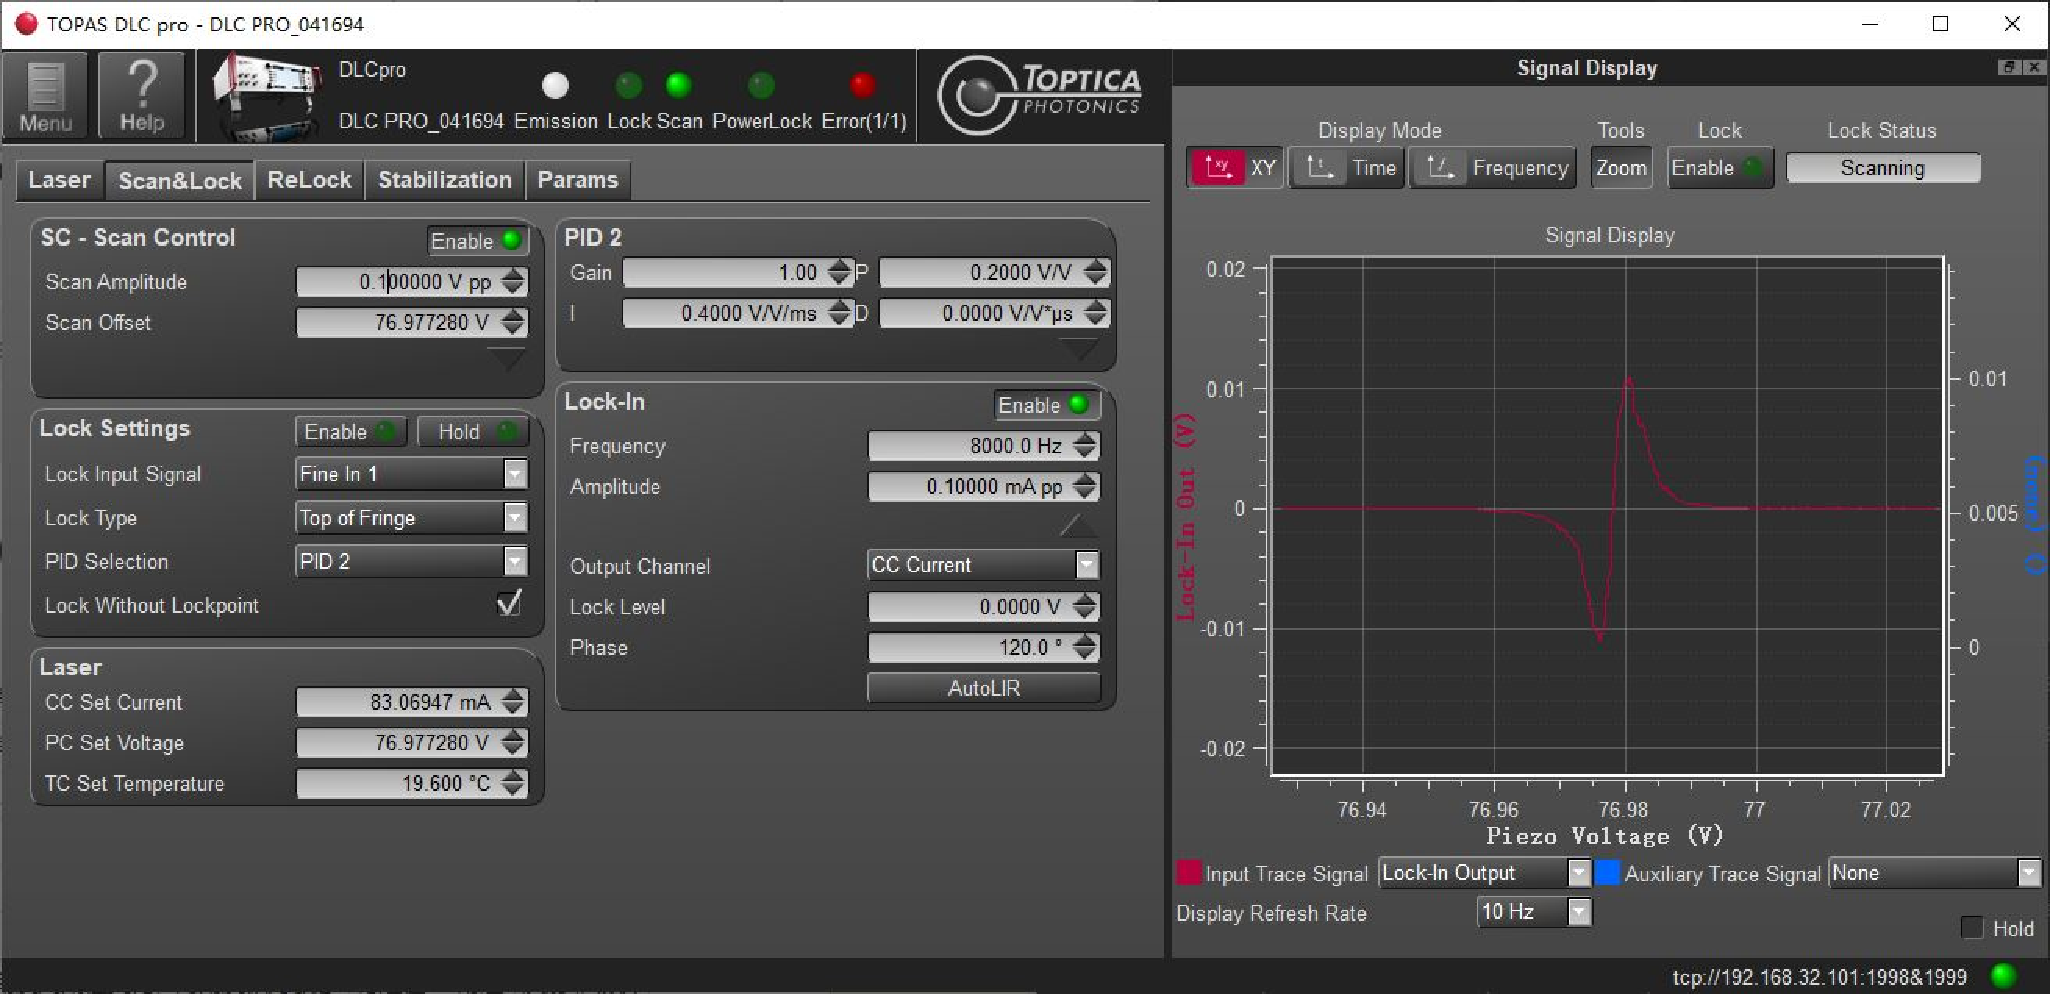
\includegraphics[width=0.8\linewidth]{fig_3_demodulated_signal.pdf}
    \caption{Demodulated signal of the optical cavity photo diode.}
\end{figure}

The results of targeting the 370 nm laser with a wavemeter are not good enough because the feedback speed is too slow. We can increase the feedback speed with the assistance of an optical cavity, as shown in Fig~\ref{fig:fig_3_optical_path_370_cavity}, which reduces the standard deviation of the output frequency of the 370 nm laser to 300 kHz. I built this optical path on a breadboard in which an optical cavity (U2; SA200-3B, Thorlabs) was placed. The outgoing light from the 370 nm laser (C9) is incident to the optical cavity. mode matching of the optical cavity is achieved by a pair of reflectors and lenses. Locking the 370 nm laser to the optical cavity is achieved by feeding the output signal of the photodiode (D1) back to the voltage signal of the 370 nm laser controller. In order to have the lock point at the point of maximum transmission light intensity of the optical cavity, I added a modulation signal to the current signal of the 370 nm laser and demodulated the signal from the photodiode (D1). This solution uses a simple optical cavity to increase the bandwidth of the laser locking. This scheme uses a simple optical cavity to increase the bandwidth of the laser locking. However, because environmental factors can cause the cavity length of the optical cavity to change, the locked frequency will change rapidly as the cavity length changes. I connected the voltage signal (S1) from the wavemeter output to the piezoelectric ceramic (P1) of the optical cavity, thus achieving a locking of the optical cavity length to the wavemeter.

\subsection{Laser modulation}

Making the laser modulation a separate module allows for modularisation of the optical path, which facilitates maintenance and testing, and also reduces the size of the optical path into the cavity, which in turn reduces the area of the breadboard where the cryogenic trap vacuum chamber is located. Optical layout of laser frequency stabilization system is shown in Fig~\ref{fig:fig_3_optical_path_370_modulate}. The main source of laser leakage during laser modulation is the higher order modes of the laser and stray light from the crystal during modulation. Adding a stage of fibre coupling can act as a spatial filter and help reduce leakage.

\begin{figure}
    \centering
    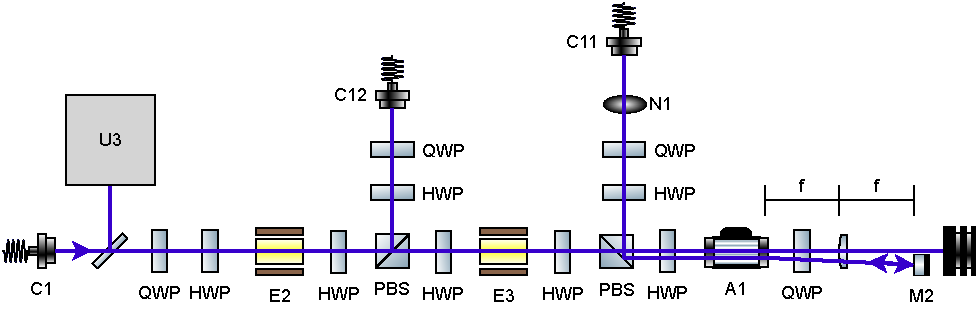
\includegraphics[width=0.8\linewidth]{fig_3_optical_path_370_modulate.pdf}
    \caption{Optical layout of laser modulation system.}
    \label{fig:fig_3_optical_path_370_modulate}
\end{figure}

Experimentally, I need to add sidebands to the 370 nm laser, the 14.7 GHz sideband (E2) for Doppler cooling and the 2.105 GHz sideband (E3) for optical pumping. the electro-optic modulator (EOM) can implement these features \cite{RN205,RN230,RN277}. The frequency and modulation depth of the sidebands can be controlled by controlling the frequency and amplitude of the EOM input microwave signal. In addition, I need to control the frequency shift and power of the 370 nm laser. This is because the difference in frequency required for Doppler cooling and state detection is approximately 12 MHz, and the frequency variation measured during calibration of the system can be compensated for by adjusting the frequency shift of the 370 nm laser \cite{RN144, RN141}. The acousto-optic modulator (AOM) provides these features. By controlling the frequency and amplitude of the microwave signal input to the AOM (A1) the frequency of the laser shift and the laser power can be controlled. However, the AOM modulation efficiency is affected by the microwave signal, as shown in Fig~\ref{fig:fig_3_optical_path_370_modulate_aom},and we need to compensate for this using software control during experimental operation.

\begin{figure}
    \centering
    \subcaptionbox{Laser intensity versus microwave power.\label{fig:fig_3_optical_path_370_modulate_aom_power}}
    {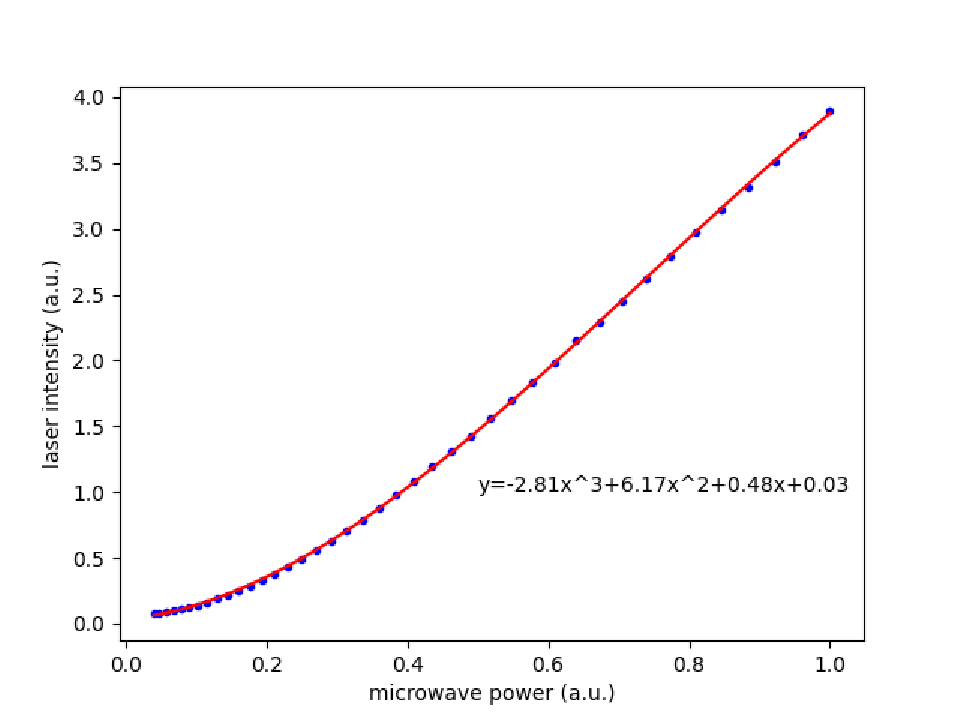
\includegraphics[width=0.4\linewidth]{fig_3_optical_path_370_modulate_aom_power.pdf}}
    \subcaptionbox{Laser intensity versus microwave frequency.\label{fig:fig_3_optical_path_370_modulate_aom_frequency}}
    {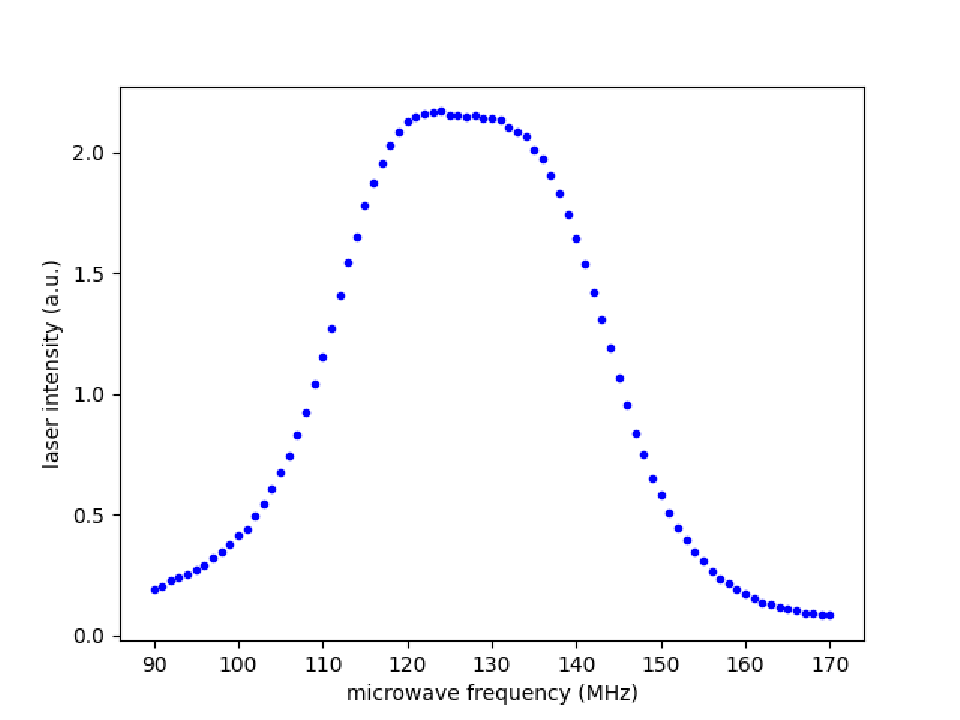
\includegraphics[width=0.4\linewidth]{fig_3_optical_path_370_modulate_aom_frequency.pdf}}
    \caption{AOM modulation efficiency influenced by microwave signal.}
    \label{fig:fig_3_optical_path_370_modulate_aom}
\end{figure}

The light source from the 370 nm laser is fed to the laser modulation module via a single-mode polarization-maintaining fibre (C1), which is reflected by a beam sampling mirror and enters the laser monitoring module (U3). A number of signal acquisition modules are integrated into the laser monitoring module to help me monitor the quality of the light source over time, including measurements of power , polarisation, laser mode and others. The main light source is modulated by two cascaded EOMs, the modulation depth of which can be maximised by adjusting the HWP. Part of the laser is coupled into the fibre (C12), which is then used for sympathetic cooling. To achieve the frequency shift, I built a double-pass configuration based on a 4f optical system, where the PBS serves to separate the incident light from the returned light by 90°, adjusting the HWP at the front to maximise the efficiency of the incident light and the HWP at the back to maximise the efficiency of the diffraction from the AOM. When the laser passes through the AOM, 0 order light is discarded and +1 order light is returned to the AOM by a 4f optical system consisting of a lens and a D-shaped pickoff mirror. The +1 order beam from the reflected beam passes through the QWP twice and is then reflected by the PBS into the fibre (C11), this light is then used for global cooling, pumping and detection. There is a mechanical shutter (N1) in front of the fibre, which serves to completely shut off the light and reduce leakage.

\subsection{Optical layout of the cryostat breadboard}

\begin{figure}
    \centering
    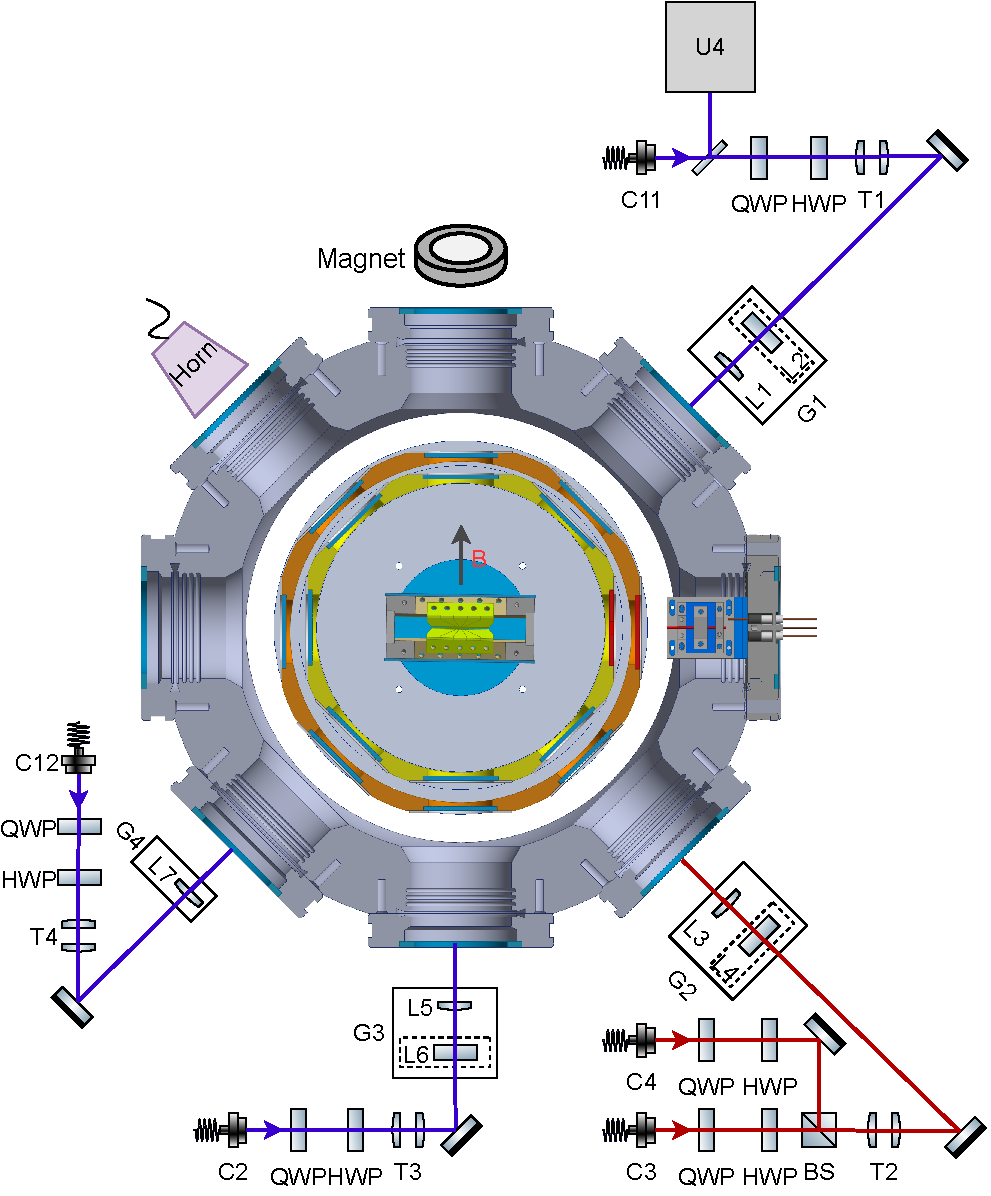
\includegraphics[width=0.8\linewidth]{fig_3_optical_path_cryostat_breadboard.pdf}
    \caption{Optical layout of the cryostat breadboard.}
    \label{fig:fig_3_optical_path_cryostat_breadboard}
\end{figure}

Due to the large base area of the cryostat, the area left for the optical path on the breadboard is relatively small. Further experimental tasks may be restricted by the number of windows. For example EIT cooling, which is important for ground state cooling in multi-ion experiments \cite{RN155, RN7, RN35, RN54}. The main function of the optical path built on the breadboard of the cryostat is to shape the beam into a specific shape and then inject it into the cavity. There are four windows on the Cryostat that are used to inject the laser. The laser light exiting the fibre collimator (C2, C3, C4, C11, C12) is first polarised by the QWP and HWP and then expanded by the lens pairs (T1, T2, T3, T4) to a suitable spot size, typically with a Gaussian diameter of approximately 10 mm. It is then incident on a long-focus lens (L1, L3, L5, L7) into the cavity and forms a small spot in the centre of the trap, typically with a Gaussian diameter of about 20 $\mu$m. The long-focus lenses are mounted on a 3-axis linear stage (G1, G2, G3, G4; M-461-XYZ-M, Newport) with a Picomotor actuator (8301NF, Newport) in each axis of the stage to achieve high precision control of the beam position.

\begin{figure}
    \centering
    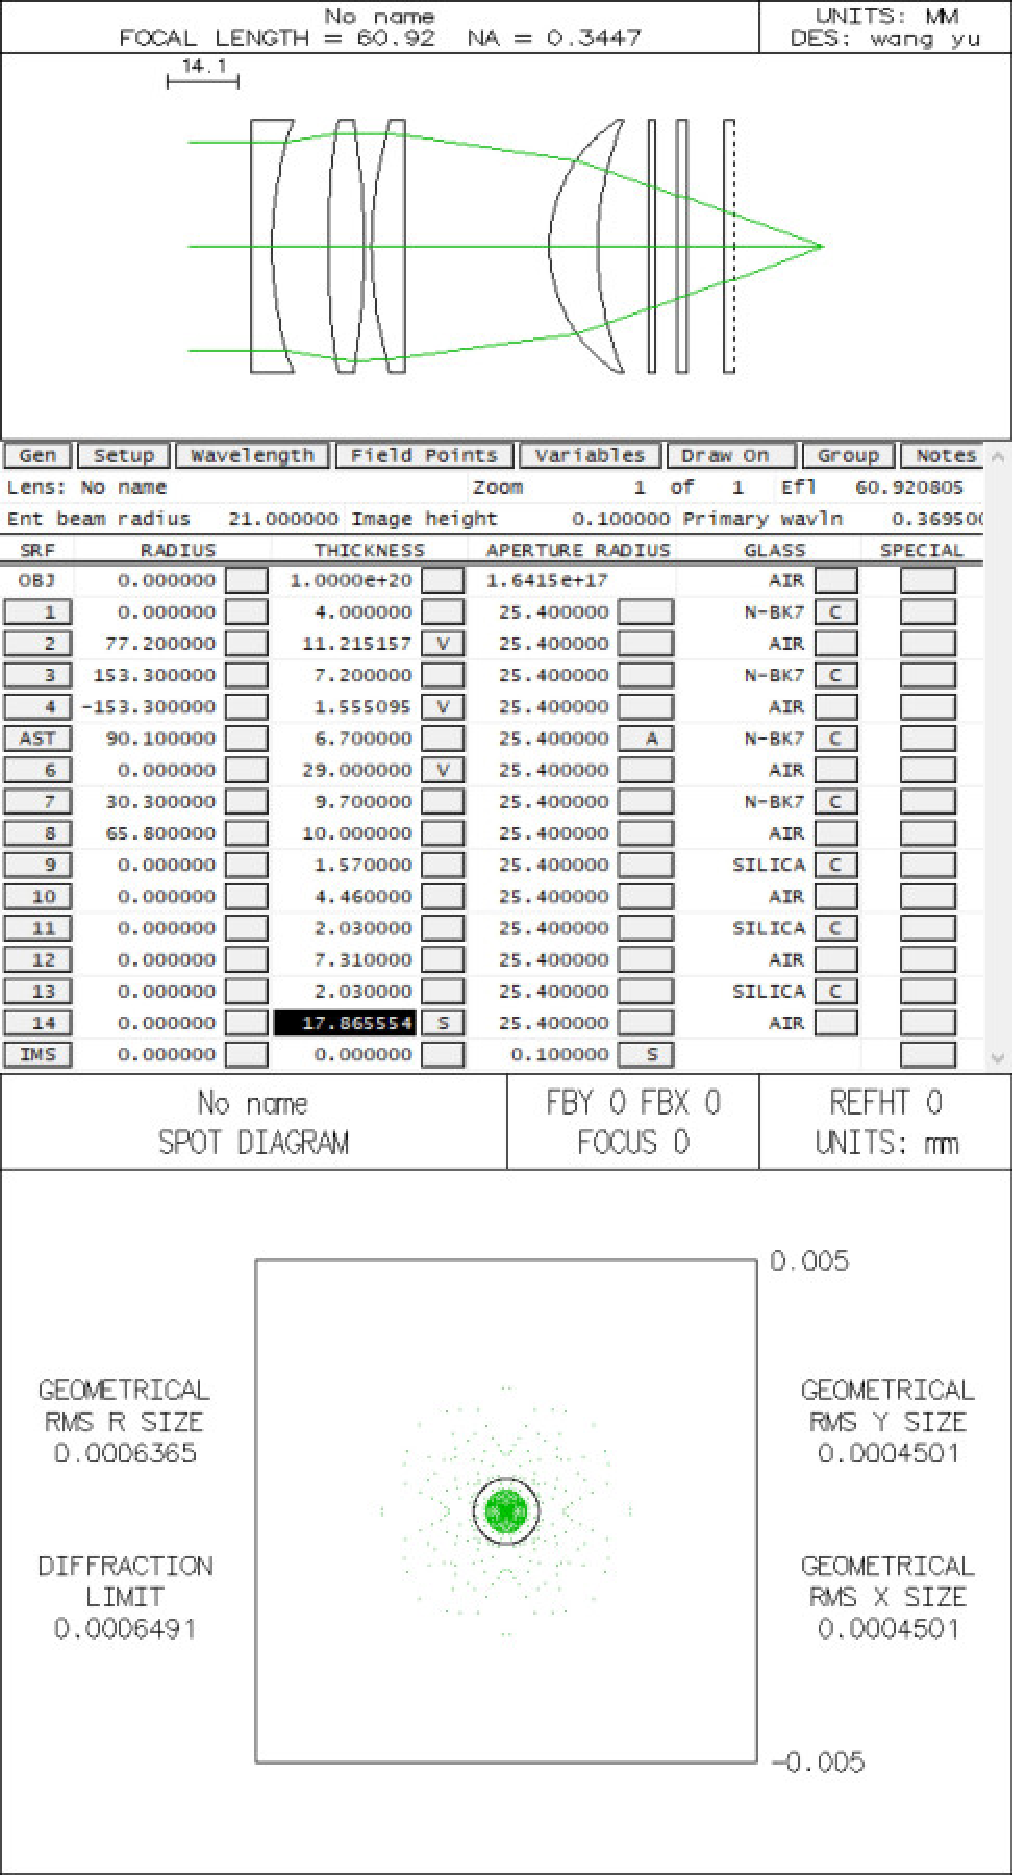
\includegraphics[width=0.4\linewidth]{fig_3_imaging_syetem_objective_design.pdf}
    \caption{Design of the objective.}
    \label{fig:fig_3_imaging_syetem_objective_design}
\end{figure}

Reducing the spot diameter at the trap is necessary to increase the power density, reduce stray light and improve the signal to noise ratio. It also helps me to monitor the displacement of the spot relative to the ions over time, which helps me to find unstable components or modules in the system at the beginning of the construction of the system. But when the length of the ion chain in the trap increases, I need some light spots to expand in the horizontal direction to about 500 $\mu$m in diameter. It is advantageous to be able to easily adjust the spot diameter in the horizontal direction. I added cylindrical lenses (L2, L4, L6) to the optical path where I needed to adjust the horizontal diameter, and by artificially introducing astigmatism, I was able to shift the horizontal focal position along the optical axis. A long-focused cylindrical lens with a focal length of approximately 1000 mm is generally used, mounted on a rotatable lens mount so that the tilt angle of the elliptical spot can be adjusted and the cylindrical lens can be removed when the elliptical spot is not required.

The stability of the 370 nm laser (C11) is so important to the experiment that a laser monitoring module (U4) has been installed at the outgoing point of the fiber. This light is global light and is required for ion loading, Doppler cooling, optical pumping, and state detection. In order to trap both ${ }^{171} \mathrm{Yb}^{+}$ and ${ }^{174} \mathrm{Yb}^{+}$, two 935 nm lasers (C3 and C4) were combined into the cavity and their function was rupumping. Combining these two 935 nm lasers at the front stage would have been a better option, but this was not done due to space planning in the laboratory. The 399 nm laser (C2) is used for ion loading and the 370 nm laser (C12) is used for sympathetic cooling.

A permanent magnet is placed in front of one window to generate a magnetic field at the centre of the trap, approximately 5 Gauss, perpendicular to the direction of the ion chain. A horn is placed in front of one of the windows to apply microwaves.

\subsection{Imaging system}

The objective is specifically designed for cryogenic trap system to collect fluorescence from the ions. The thickness of the glass inside the chamber is 5.63 mm. The numerical aperture of the fluorescence collection objective has to be as large as possible and the currently used objective has a numerical aperture of approximately 0.35. The design of the objective is shown in Fig~\ref{fig:fig_3_imaging_syetem_objective_design}

We use the PMT (Hamamatsu H11890) for State Detection of one single ion and the EMCCD (Andor iXon Ultra 888) for State Detection of multiple ions, where the average SPAM error is 3\%.

\begin{figure}
    \centering
    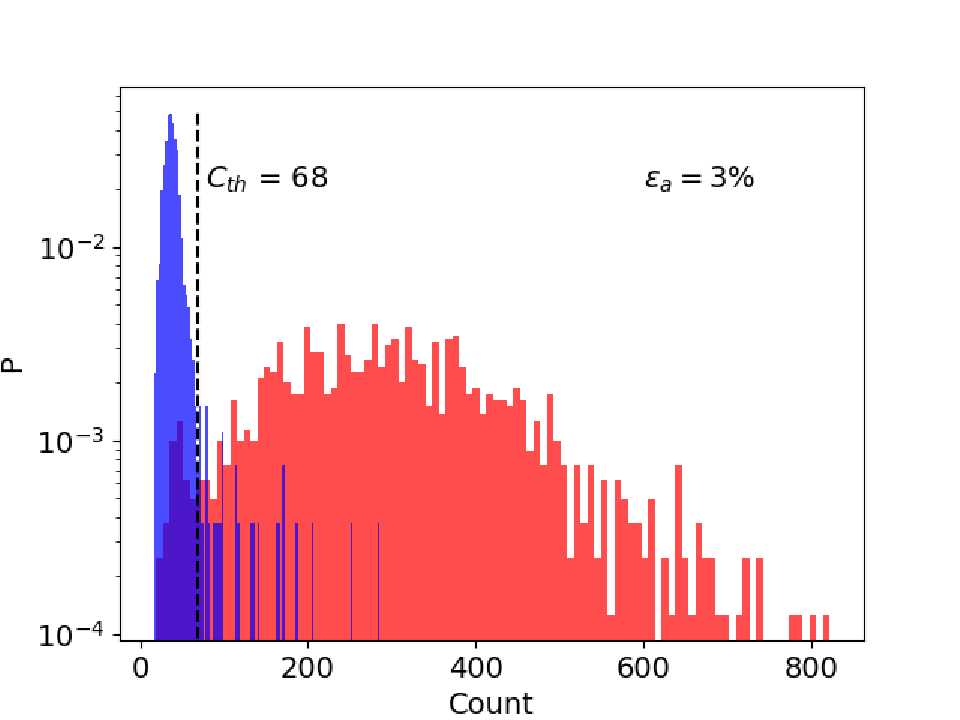
\includegraphics[width=0.5\linewidth]{fig_3_imaging_syetem_spam_error.pdf}
    \caption{Detection error analysis.}
    \label{fig:fig_3_imaging_syetem_spam_error}
\end{figure}




\section {Coherent microwaves}

\begin{table}
    \centering
    \caption{Measurement of microwave frequency and rabi rate.}
    \begin{tabular}{lll}
        \toprule
        Energy level   & microwave frequency & $\pi$-time \\
        \midrule
        $|1,0\rangle$  & 200.0344 MHz        & 122.3      \\
        $|1,-1\rangle$ & 188.0974 MHz        & 78.3       \\
        $|1,1\rangle$  & 211.9524 MHz        & 78.2       \\
        \bottomrule
    \end{tabular}
    \label{tab:microwave}
\end{table}

The system is outfitted with a microwave horn in order to coherently drive global spin rotations.
The $|\downarrow\rangle$ and $|\uparrow\rangle$ states are directly coupled by a magnetic dipole moment, so the
microwaves can directly drive rotations. Microwave signals are generated by mixing high frequency signals (Rohde \& Schwarz SMB-100A, 11 dBm @ 12.4428 GHz) with low frequency signals (Analog Devices AD9910, around 200 MHz). The signals then passes through a high frequency amplifier and is output to a microwave speaker. Measurement of microwave frequency and rabi rate for different energy levels is shown in Table~\ref{tab:microwave}. Here the microwave frequency is added to 12.4428 Ghz to get the absolute frequency of the corresponding energy level.

% !TeX root = ./PhDThesis.tex

\chapter{Cryogenic experimental technique}

\section{Cool-down and warm-up procedures}

The cryogenic trapped-ion system is a relatively complex experimental system, and we need the system to be stable over a long period of time so that the reproducibility of the measurement results is high. Although the cryostat's core component, the cold head, can run continuously for more than 10000 hours, the maximum time this cryostat can run continuously is limited by the stability of the power supply, the stability of the laboratory temperature and humidity, and whether the exchange gas space is leaking, as shown in Fig~\ref{fig:fig_4_exchange_gas_space_leakage}. It took us about three years to get the system into a stable long-term state, after which we conducted a series of physical experiments on the experimental platform. However, during the three-year commissioning process, we inevitably need to conduct the cycle of cool-down, malfunction, warm-up, and upgrade, during which the standardized operation helps to make the physical parameters of the system more repeatable, so we have developed a standardized operation procedure for this system.

\subsection{Maintenance of the exchange gas space}

\begin{figure}
    \centering
    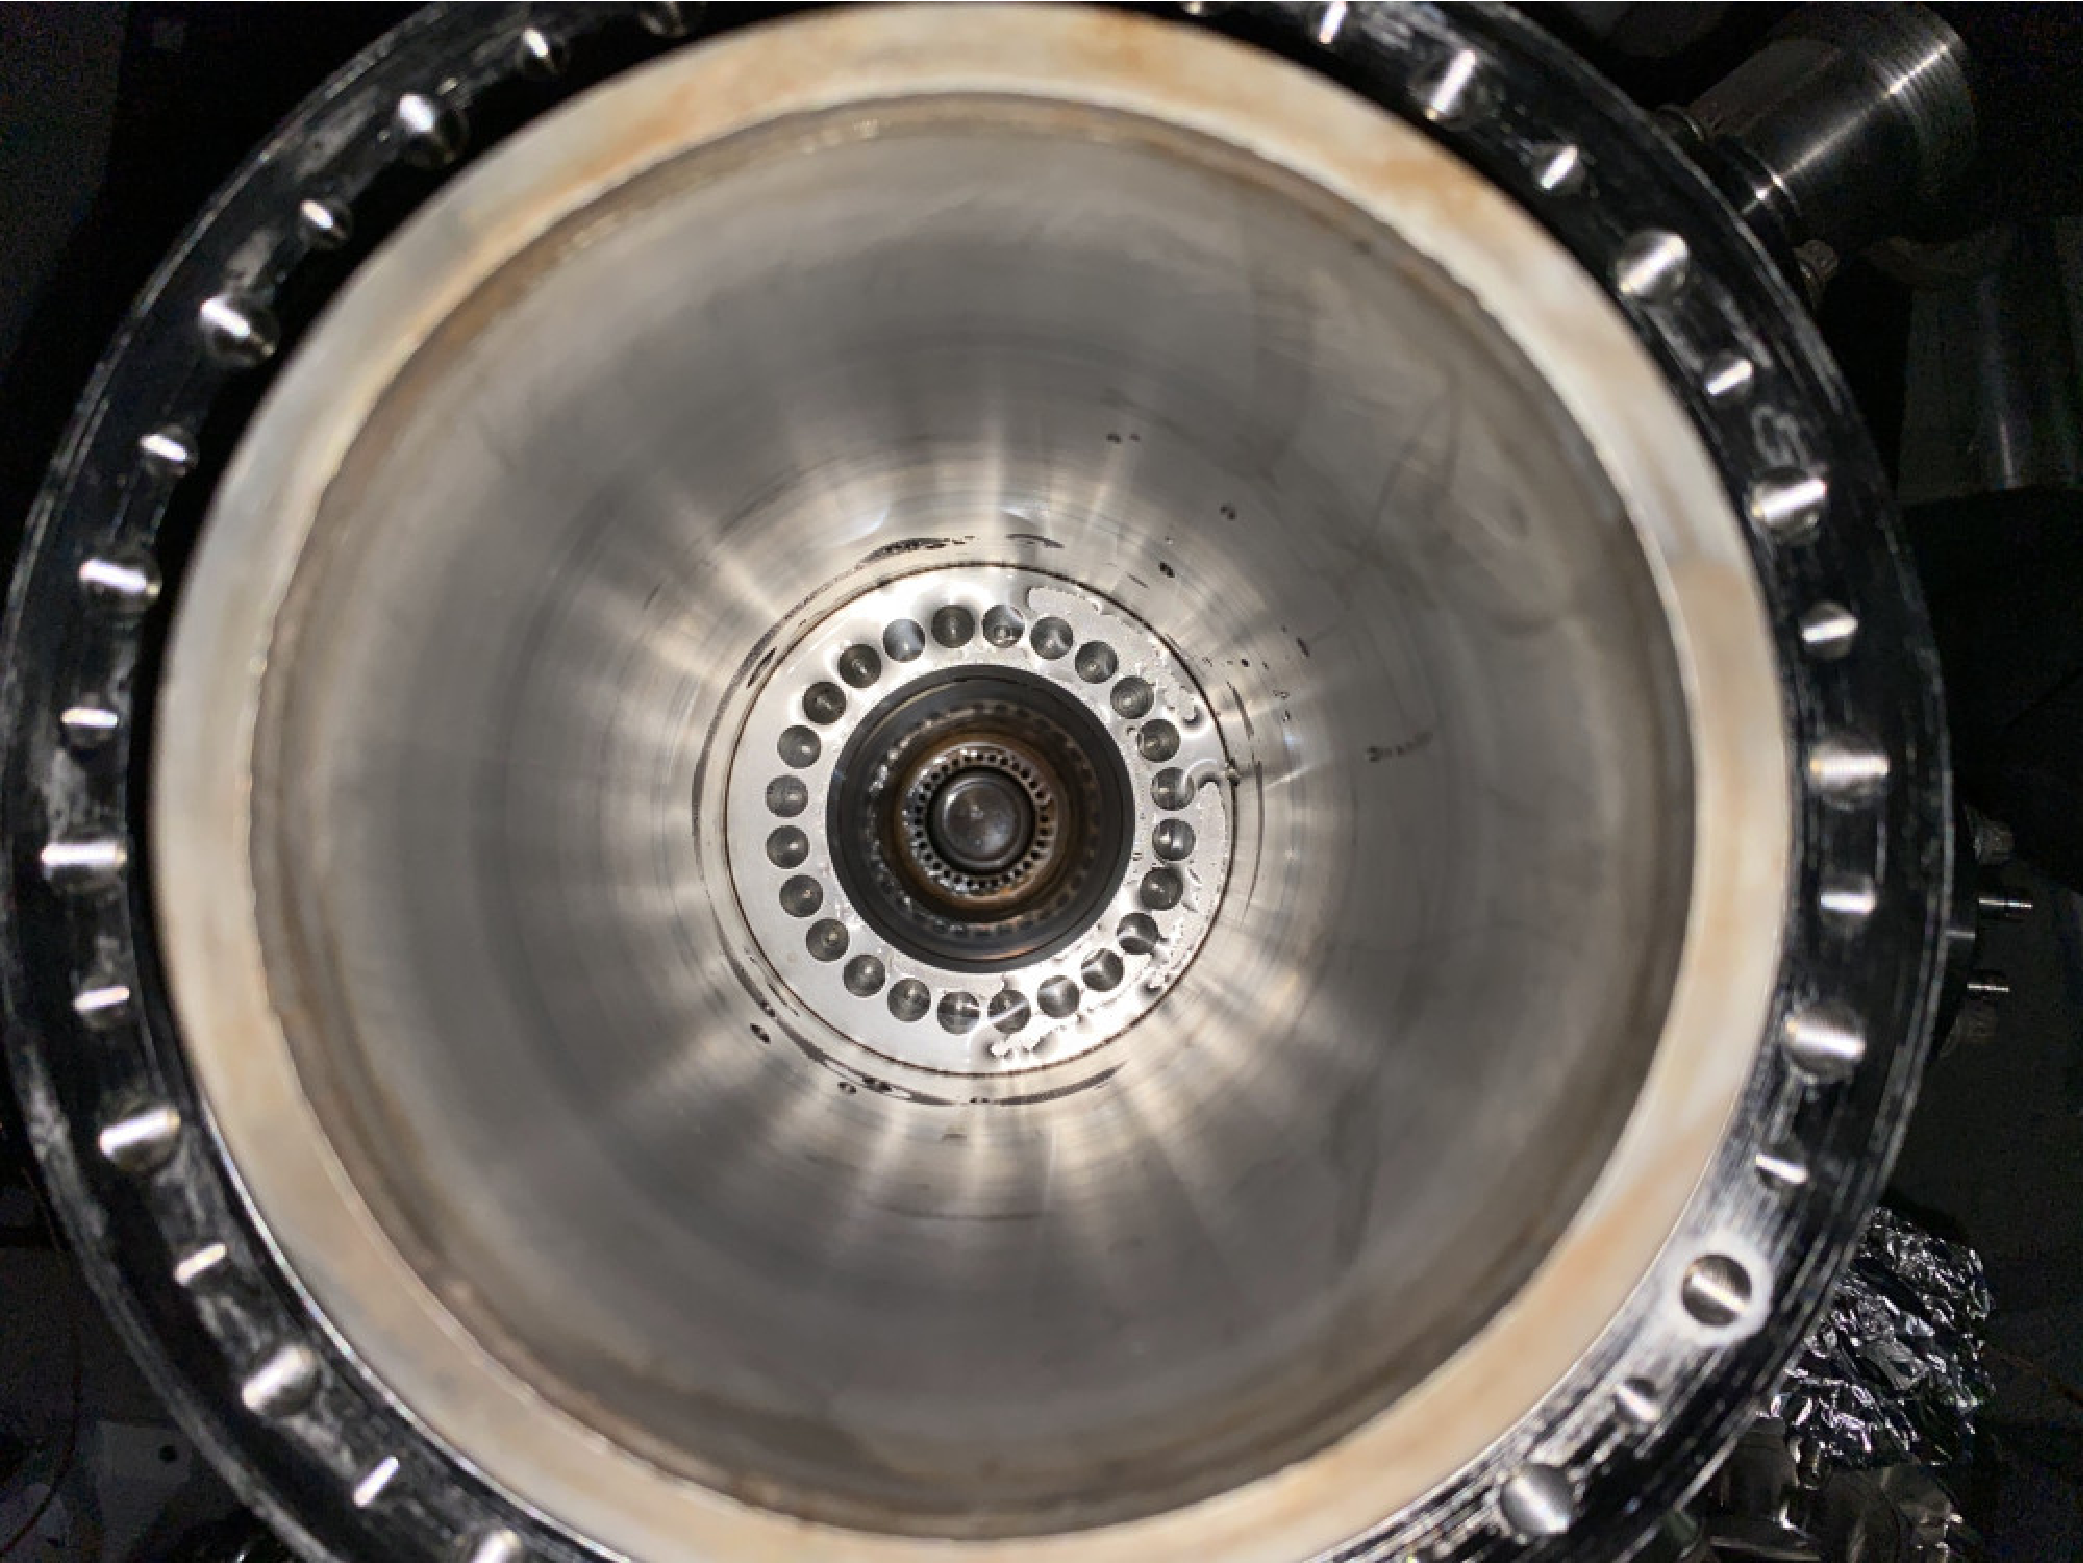
\includegraphics[width=0.8\linewidth]{fig_4_exchange_gas_space_leakage.pdf}
    \caption{Observation of leakage in the exchange gas space.}
    \label{fig:fig_4_exchange_gas_space_leakage}
\end{figure}

If the cold head does not need to be removed for servicing, the exchange gas space does not require frequent maintenance and is always in an independent and stable state, whether it is being cooled down or warmed up.

The exchange gas space uses helium gas with a purity of 99.999\%. When we expose the exchange gas space to atmosphere or when it is first used, the internal gas needs to be purified. According to the cryostat manufacturer's recommendations, a purification is also required after several months of continuous running, but this is not normally done when the system is stable for a long period of time. How often the exchange gas space needs to be purified depends on the rate of impurity gases (nitrogen, oxygen, water vapour etc.) leaking in from the atmosphere.

When we need to purify the helium gas in the exchange gas space, the exchange gas space is first evacuated continuously for 0.5 hours with a dry scroll pump (Agilent IDP-7), then the valve connected to the dry scroll pump is closed and the valve connected to the helium gas is opened. The auto gas charging system will then raise the pressure to 1.03 bar and finally we close the valve to the helium gas. In general, the above operation is repeated three times to purify the helium gas in the exchange gas space.

When we need to cool down or warm up the system, and also when the system is running at low temperatures for a long time, we simply open the valve to the helium gas and keep the auto gas charging system running steadily.

\subsection{Cool-down}

\begin{figure}
    \centering
    \subcaptionbox{Temperature vs. time.}
    {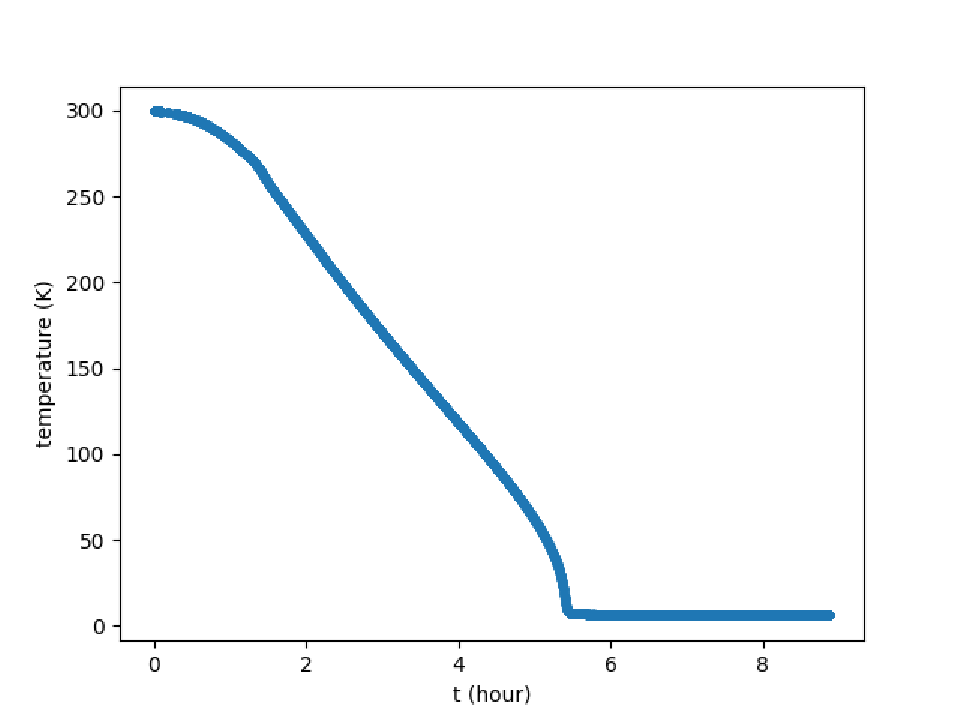
\includegraphics[width=0.4\linewidth]{fig_4_cool_down_temperature.pdf}}
    \subcaptionbox{Pressure vs. time.}
    {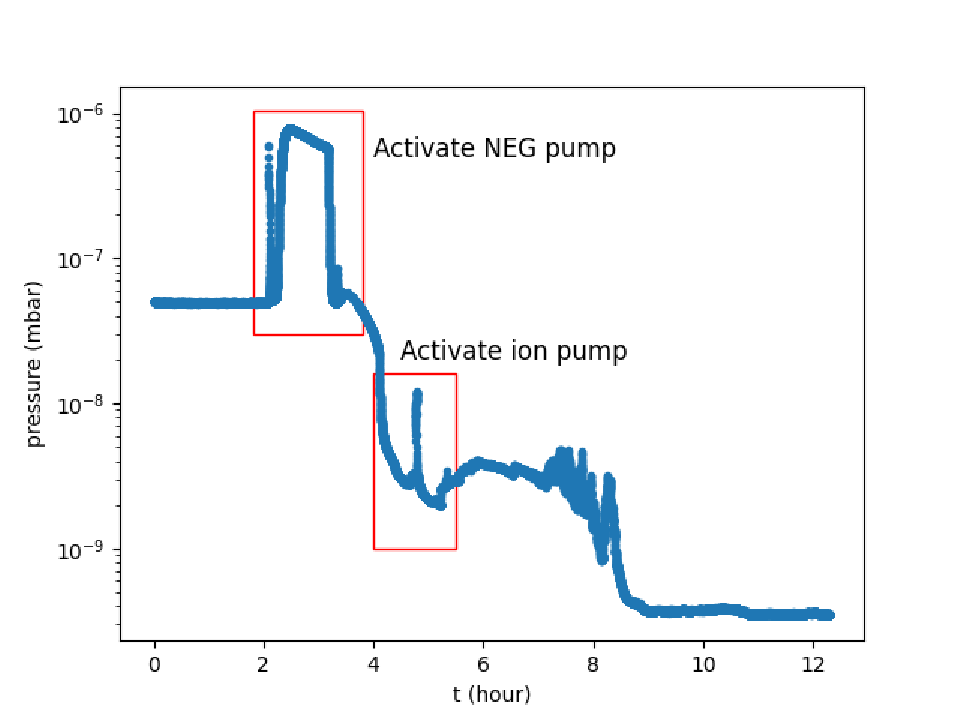
\includegraphics[width=0.4\linewidth]{fig_4_cool_down_pressure.pdf}}
    \caption{Cryostat temperature and pressure over time during a cool-down.}
\end{figure}

In the cool-down procedure, the physical parameters of the vacuum chamber are mainly adjusted and observed. The vacuum chamber is first connected to a turbo-molecular pump (TPS-compact Turbo Pumping System) via the angle valve and after approximately 48 hours of continuous operation the vacuum chamber reaches a vacuum level close to UHV. The ion gauge is switched on and reaches an indication of $5 \times {10}^{-8}$ mbar, at which point we do not need to degas the ion gauge as the room temperature zone of the vacuum chamber does not eventually fall below $1 \times {10}^{-10}$ mbar. Now we need to perform a time limited activation of the NEG Pump for 1 hour, then we perform several degas of the Ion Pump and keep the Ion Pump on. Now that the activation of the NEG-Ion Pump is complete, we close the angle valve and wait about 1 hour for the ion gauge to gradually decrease to $3 \times {10}^{-9}$ mbar, when the vacuum chamber reaches the UHV vacuum level. We turn on the cold head and the temperature stabilize system, which will finish cooling down within 5 hours, but the system will not reach final stabilization for more than 24 hours. The temperature of the 4 K stage is finally stabilised at 6 K and the ion gauge is stabilised at $3 \times {10}^{-10}$ mbar.

\subsection{Warm-up}

\begin{figure}
    \centering
    \includegraphics[width=0.4\linewidth]{fig_4_warm_up_temperature.pdf}
    \caption{Cryostat temperature over time during a warm-up.}
\end{figure}

The warm-up procedure is much easier than the cool-down procedure because we do not need to obtain UHV during this process. we turn off the cryogenic and vacuum related instruments: the NEG-Ion pump, the ion gauge, the cold head. We can use the heater in the temperature stabilize system to heat the cryostat to speed up the warming process to room temperature, which takes about 24 hours or more. The system can also be allowed to warm up naturally to room temperature, which takes about 48 hours or more. Next, if necessary, we can move the cryostat into the service area for servicing. Before moving it out, we need to record the readings of all optical and electrical instruments. As the imaging system is embedded in the re-entrant window, we usually need to remove the objective lens.

\section{Characterization of the vibration}

A stimulated two-photon Raman process using a pulsed 355 nm laser is used to produce the spin-spin interactions. Because of this, any displacement of the ion chain that occurred during the contact period that was on the order of the wavelength of the Raman laser would create an undesirable phase shift in the ions. As a result, it is of the most importance to minimize the vibration that occurs inside this Gifford-McMahon closed-cycle cryostat.

\subsection{The Michelson interferometer}

Although there are many different instruments for measuring vibration signals, such as capacitive sensors for vibration measurement, most of them are not suitable for use in our systems. Measurement of vibration signals in UHV systems at cryogenic temperatures is mainly done by non-contact measurement, and the use of lasers is a very good solution for non-contact measurement, which is also suitable for our systems. There are two main solutions for measuring position information based on laser, the laser Doppler vibrometer and the laser interferometer. The Laser Doppler vibrometer measures the spectrum of vibration signals mainly according to the Doppler principle. Its measurement accuracy is dependent on the speed of the object's movement and is therefore very accurate for high frequency signals. However, the cryostat vibration signal does not generally exceed 200 Hz. we are concerned on the one hand with vibration signals that may change the relative phase between the ion and the laser during the laser manipulation sequence, which can usually be measured on the cryostat at frequencies between 10 Hz and 200 Hz and amplitudes between 1 nm and 100 nm. In this frequency range, the laser Doppler vibrometer is not very accurate. On the other hand, we are concerned with the displacement of the trap relative to the optical path over a long experimental period, e.g. one hour. The accuracy of the Laser Doppler vibrometer in measuring this long term drift is very low, typically measured with an error of no less than 100nm, mainly due to the fact that most laser Doppler vibrometers use a velocity integration method to calculate the displacement.

\begin{figure}
    \centering
    \includegraphics[width=0.8\linewidth]{fig_3_optical_path_370_Interferometer.pdf}
    \caption{Optical layout of the Michelson interferometer.}
    \label{fig:fig_3_optical_path_370_Interferometer}
\end{figure}

The laser interferometer is a class of instrument that is commonly used for measuring displacement and its principle and performance meet our requirements for vibration measurement. Unlike the more industrially used dual-frequency laser interferometer, I have built a very simple Michelson interferometer in my laboratory, as shown in Fig~\ref{fig:fig_3_optical_path_370_Interferometer}, because commercially available laser interferometers are generally not compatible with ultra-high vacuum systems and are not suitable for use in very compact chambers.

Experimentally we will fix a small reflector, about 6mm in diameter, to the trap holder, which is located in the 4 K reigon inside the cryostat. We have tried using silver epoxy to hold the mirror to the trap holder, but usually the epoxy is detrimental to our ability to obtain XHV and it would be better to use UHV compatible plastic screws to hold the mirror in place. Since it is so well fixed, we believe that the trap displacement can be calculated by measuring the change in the relative optical path of the reflector. The laser is emitted from outside the chamber and then returned from inside the chamnber through six transmissions and one reflection from the reflector, 4 K shield glass, 40 K shield glass and the viewport of the vacuum chamber. Therefore, it is often necessary to place an optical coating on the surface of these glasses to increase the transmission and reflectivity and thus improve the signal-to-noise ratio of the interferometric signal. If the coating of the glass does not match the wavelength of the laser, some measurement accuracy may be lost, but this is not fatal and it is advantageous to relax the wavelength range required for the optical coating for a more scalable cryostat design. We have tried using retroreflectors instead of mirrors. Since retroreflectors are not sensitive to changes in angle, if the reflector is disturbed by a vibration pulse during the measurement resulting in a change in angle, the signal-to-noise ratio of the interferometric signal is significantly reduced, which can be avoided by using a retroreflector. However, due to the UHV and the very small size of the chamber, the signal-to-noise ratio of the interferometric signal from the retroreflector is significantly lower than that of the interferometric signal from the reflector. On the other hand we have optimised the design to reduce the vibrations and the angular shift generated by this pulsed signal is suppressed, so that for systems with small vibrations the use of a reflector is a better option.

A Michelson interferometer-based measurement solution requires a very stable laser source. Or rather the measurement error is directly related to the jitter of the laser source. This is because we do not currently use a solution similar to the Mach-Zehnder interferometer, so the PID can only be locked to the rising edge of the fringe of the signal, and the addition of a modulation module would reduce the interference caused by laser source jitter, i.e. improve the signal-to-noise ratio. Experimentally, the coherence length of a single-frequency laser should be much greater than 1 m, and the power and polarisation jitter should ideally be less than 1\%, and at worst no more than 5\%. Fortunately, the 370nm laser we use meets these requirements and can be used as the laser source for the laser interferometer, thus reducing the cost of building the instrument ourselves. One arm of the interferometer comes from the return laser from the reflector on the trap holder and the other arm comes from the return laser from the reflector fixed to the optical table, so we can measure the change in the optical range of the trap relative to the optical table. The interferometric laser is directed at the photodiode and the photocurrent is passed through the transimpedance amplifier to generate an interference voltage signal. The error signal generated by the PID module is then output to a high voltage amplifier, which generates a voltage signal to drive the piezoelectric ceramic on the optical stage reflector. This creates a phase-locked loop and by reading the value of the voltage signal from the piezoelectric ceramic we can determine the change in the optical path of the reflector on the trap holder. The feedback bandwidth of this loop is approximately 1kHz, which is limited by the bandwidth and linear operating range of the piezoelectric ceramic. We have increased the feedback bandwidth of the phase-locked loop by choosing to use a high bandwidth piezoelectric ceramic and a small mass of reflector as a load on the piezoelectric ceramic.

\subsection{High-precision long-term vibration measurement}

Before a mature cryostat is developed, we usually debug some experimental phenomena and experimental parameters repeatedly in our experiments. These problems due to the immaturity of the cryostat can arise from mechanical design, optical errors and electrical noise. We usually analyse these problems by comparing a cryogenic trap system with an room-temperature trap system, which is simpler in structure and therefore more stable. So a stable cryostat can greatly guarantee the rapid forward movement of our experimental process. Some stability may be necessary, such as vibrations in the laser manipulation sequence, which may affect the quantum gate fidelity, and long-term drift, which may affect the possibility of individual addressing. It is therefore necessary to experimentally measure the trapped ions with respect to the laser's optical path precisely and over a long period of time to achieve passive stabilisation of the various parameters of the cryostat.

Before carrying out the measurements, I calibrated the instrument. The wavelength of the laser coming out of the single-mode polarisation-maintain fibre (C10) was 370 nm, and I first checked the stability of the power and polarisation of the light coming out of the fibre by connecting it to a power meter and a polarisation analyser respectively. After confirming the stability of the laser source, I also checked the long-term stability of the interference signal, mainly by measuring the stability of the maximum and minimum values of the interference signal. I used epoxy glue to glue the reflector, piezoelectric ceramic and mirror mount together. Although the product manual for piezoelectric ceramics gives a relationship between displacement and voltage, in practice I have found that the linearity of these mirrors varies considerably from one production to the next, and in some cases the linearity changes after a few months. It is therefore necessary to calibrate the relationship between the displacement of the mirror and the voltage. I use a flipper mirror to change one arm of the interferometer from the cavity to another mirror on the optical stage, as the change in the interference signal at this point is so small that it can be assumed that there is no additional vibration. I applied a drive signal to the piezoelectric ceramic of the reflector to be calibrated and could see the interferometric signal oscillate. The relationship between the driving voltage and the interference signal deviates from sinusoidal oscillations because the driving relationship is not linear and the change in the angle of the mirror during the application of the driving signal causes a consequent change in the contrast of the interference signal. I calculated the optical path by selecting the eigenpoints of the interferometric maximum and minimum values. In the end, I can calculate the linear coefficients of the driving voltage and displacement for each manufactured reflector. In principle I could measure the vibration signal of the trap immediately, but to ensure that the measurement was correct I carried out a simulation experiment. By applying a drive signal to the mirrors of the other arm of the interferometer, the linear coefficients of voltage and displacement of each mirror were of course calibrated, and then the drive signal of the measured mirrors was read out. A comparison of these two signals gives the measurement accuracy.

\subsection{Minimize vibration of the cryostat}

In our laboratory, the vibration of the optical elements on the floating optical platform is around a few tens of nm, and our ultimate goal is to reduce the vibration of the cryostat to this order of magnitude. In our initial cryostat setup, the vibrations were in the order of a few hundred nm, half of which stemmed from the instability of the internal structure of the chamber and the other half from the vibrations caused by the cold head. Since vibrations of several hundred nm were also measured when the chiller was switched off, we decided to reinforce the internal structure of the cavity. In addition to the vibrations over a short period of time, the ions produce a translation of 1-10 $\mu$m during the process of doing the experiment, which indicates a long drift inside the chamber in response to environmental changes, as evidenced by the interferometer measurements. We first modified the support point in the 4 K region of the cavity. Previously the support passed through the whole of the exchange gas region and was therefore subject to long drift due to changes in the environment of the exchange gas region. We have now moved the support to the 300 K region and shortened the support material. Although we will lose some refrigeration capacity, we have solved the problem of long drift. We found that the suspension design did not allow enough support points for the 4 K shield and 40 K shield, so we added PEEK connectors to the bottom of the shield. By optimising the structural design of the cavity, we managed to solve the vibration and long drift problems.



\section {Obtain impedance match of helical resonator}

If the RF voltage is applied directly from the RF amplifier to the ion trap, the following problems may be caused. An impedance mismatch between the RF amplifier and the ion trap will cause the RF signal to be reflected from the ion trap, resulting in power dissipation in the output impedance of the RF amplifier. The RF amplifier will also input noise into the ion trap, which may lead to heating of the ions. So we connect the output of the RF amplifier to a helical resonator. Due to the damping effect of the output impedance of the RF amplifier, connecting the helical resonator directly to the RF amplifier will reduce the quality factor of the spiral resonator, so this connection can be achieved by capacitive or inductive coupling, thus decoupling the helical resonator from the resistive output impedance of the RF amplifier, as well as giving the spiral resonator a high quality factor. This technique allows the impedance of the ion trap and the RF amplifier to be matched by varying the coupling, thereby reducing the reflected power and therefore the output power of the RF amplifier when the voltage required to generate the ion trap is reduced. Passing the output of the RF amplifier through a resonator allows the noise to be filtered and its contribution to the ion heating to be reduced to the greatest extent possible due to the high quality factor and narrow bandwidth of the resonator.

This shows that it is very important to obtain a high quality factor and to achieve impedance matching for the blade trap. For the room-temperature trap, we can feed the RF signal into the blade trap via feedthrough after the vacuum chamber has been established, so we can assemble and test the helical resonator that generates the RF signal on the optical stage. For the cryogenic trap we need to place the helical resonator inside the vacuum chamber. This reduces the circuit resistance to obtain a high quality factor, maintains the relative temperature stability of the helical resonator and the blade trap, and reduces electrical noise by reducing the circuit length and temperature. At the same time the quality factor is very much improved at low temperatures due to the reduced resistance compared to a room-temperature trap. However, the impedance matching is disrupted due to the reduced resistance at low temperatures and we need to find a way to achieve impedance matching at low temperatures. The impedance matching parameters can be found using the dichotomous method by repeated warm-up and cool-down test operations, but a single warm-up operation lasting at least 2 days is too cumbersome. By modelling the RF system and measuring the system parameters in a single run, we can find a convenient way to adjust the impedance matching.



% 其他部分
\backmatter

% 参考文献
\bibliography{ref/refs}  % 参考文献使用 BibTeX 编译
% \printbibliography       % 参考文献使用 BibLaTeX 编译

% 附录
% 本科生需要将附录放到声明之后,个人简历之前
\appendix
% % !TeX root = ../thuthesis-example.tex

\begin{survey}
\label{cha:survey}

\title{Title of the Survey}
\maketitle


\tableofcontents


本科生的外文资料调研阅读报告。


\section{Figures and Tables}

\subsection{Figures}

An example figure in appendix (Figure~\ref{fig:appendix-survey-figure}).

\begin{figure}
  \centering
  \includegraphics[width=0.6\linewidth]{example-image-a.pdf}
  \caption{Example figure in appendix}
  \label{fig:appendix-survey-figure}
\end{figure}


\subsection{Tables}

An example table in appendix (Table~\ref{tab:appendix-survey-table}).

\begin{table}
  \centering
  \caption{Example table in appendix}
  \begin{tabular}{ll}
    \toprule
    File name       & Description                                         \\
    \midrule
    thuthesis.dtx   & The source file including documentaion and comments \\
    thuthesis.cls   & The template file                                   \\
    thuthesis-*.bst & BibTeX styles                                       \\
    thuthesis-*.bbx & BibLaTeX styles for bibliographies                  \\
    thuthesis-*.cbx & BibLaTeX styles for citations                       \\
    \bottomrule
  \end{tabular}
  \label{tab:appendix-survey-table}
\end{table}


\section{Equations}

An example equation in appendix (Equation~\eqref{eq:appendix-survey-equation}).
\begin{equation}
  \frac{1}{2 \uppi \symup{i}} \int_\gamma f = \sum_{k=1}^m n(\gamma; a_k) \mathscr{R}(f; a_k)
  \label{eq:appendix-survey-equation}
\end{equation}


\section{Citations}

Example citations in appendix.
\cite{abrahams99tex}
\cite{salomon1995advanced}
\cite{abrahams99tex,salomon1995advanced}


\bibliographystyle{unsrtnat}
\bibliography{ref/appendix}

\end{survey}
       % 本科生:外文资料的调研阅读报告
% % !TeX root = ./PhDThesis.tex

\begin{translation}
\label{cha:translation}

\title{书面翻译题目}
\maketitle

\tableofcontents


本科生的外文资料书面翻译。


\section{图表示例}

\subsection{图}

附录中的图片示例(图~\ref{fig:appendix-translation-figure})。

\begin{figure}
  \centering
  \includegraphics[width=0.6\linewidth]{example-image-a.pdf}
  \caption{附录中的图片示例}
  \label{fig:appendix-translation-figure}
\end{figure}


\subsection{表格}

附录中的表格示例(表~\ref{tab:appendix-translation-table})。

\begin{table}
  \centering
  \caption{附录中的表格示例}
  \begin{tabular}{ll}
    \toprule
    文件名             & 描述                 \\
    \midrule
    thuthesis.dtx   & 模板的源文件,包括文档和注释     \\
    thuthesis.cls   & 模板文件               \\
    thuthesis-*.bst & BibTeX 参考文献表样式文件   \\
    thuthesis-*.bbx & BibLaTeX 参考文献表样式文件 \\
    thuthesis-*.cbx & BibLaTeX 引用样式文件    \\
    \bottomrule
  \end{tabular}
  \label{tab:appendix-translation-table}
\end{table}


\section{数学公式}

附录中的数学公式示例(公式\eqref{eq:appendix-translation-equation})。
\begin{equation}
  \frac{1}{2 \uppi \symup{i}} \int_\gamma f = \sum_{k=1}^m n(\gamma; a_k) \mathscr{R}(f; a_k)
  \label{eq:appendix-translation-equation}
\end{equation}


\section{文献引用}

文献引用示例\cite{abrahams99tex}。


\appendix

\section{附录}

附录的内容。


% 书面翻译的参考文献
\bibliographystyle{unsrtnat}
\bibliography{ref/appendix}

% 书面翻译对应的原文索引
\begin{translation-index}
\nocite{salomon1995advanced}
\bibliographystyle{unsrtnat}
\bibliography{ref/appendix}
\end{translation-index}

\end{translation}
  % 本科生:外文资料的书面翻译
% !TeX root = ./PhDThesis.tex

\chapter{补充内容}

附录是与论文内容密切相关、但编入正文又影响整篇论文编排的条理和逻辑性的资料,例如某些重要的数据表格、计算程序、统计表等,是论文主体的补充内容,可根据需要设置。


\section{图表示例}

\subsection{图}

附录中的图片示例(图~\ref{fig:appendix-figure})。

\begin{figure}
  \centering
  \includegraphics[width=0.6\linewidth]{example-image-a.pdf}
  \caption{附录中的图片示例}
  \label{fig:appendix-figure}
\end{figure}


\subsection{表格}

附录中的表格示例(表~\ref{tab:appendix-table})。

\begin{table}
  \centering
  \caption{附录中的表格示例}
  \begin{tabular}{ll}
    \toprule
    文件名             & 描述                 \\
    \midrule
    thuthesis.dtx   & 模板的源文件,包括文档和注释     \\
    thuthesis.cls   & 模板文件               \\
    thuthesis-*.bst & BibTeX 参考文献表样式文件   \\
    thuthesis-*.bbx & BibLaTeX 参考文献表样式文件 \\
    thuthesis-*.cbx & BibLaTeX 引用样式文件    \\
    \bottomrule
  \end{tabular}
  \label{tab:appendix-table}
\end{table}


\section{数学公式}

附录中的数学公式示例(公式\eqref{eq:appendix-equation})。
\begin{equation}
  \frac{1}{2 \uppi \symup{i}} \int_\gamma f = \sum_{k=1}^m n(\gamma; a_k) \mathscr{R}(f; a_k)
  \label{eq:appendix-equation}
\end{equation}


% 致谢
% !TeX root = ./PhDThesis.tex

\begin{acknowledgements}
  始于初秋,终于盛夏. 每一段学习的旅程好像都是这样,在秋高气爽的九月入学,在烈日炎炎的六月毕业。清华大学给我提供了世界一流的学习科研平台,我有幸在这里度过了五年的难忘时光,期间我得到了老师、家人、同学、朋友的关怀和帮助。在此我向他们表示我最诚挚的谢意。国力日渐强盛是科技进步的保障,在此我向众志成城,共同战胜新冠疫情的中国人民致以崇高的敬意。

  衷心感谢导师段路明教授对我的精心指导,他的言传身教将使我终生受益。段路明教授是一位理论物理学大师:他完成了量子信息领域一些开创性的工作,提出实现长距离量子通信网络的量子中继方案,被国际同行誉为“DLCZ”方案,为该领域的奠基性方案;他提出通过量子网络互联进行规模化量子计算的方案,为近期离子量子计算的规模化发展奠定了理论基础。段路明教授还是一位实验物理学大师,目前超导和离子阱量子计算被广泛认为是最有可能实现通用量子计算的物理体系,此外在光量子、NV色心、冷原子等体系上的研究也取得了突破性进展,段路明教授对于所有这些领域都有深刻理解,包括理论上和实验上的深刻理解。确立正确的研究方向是科研工作的重点,得益于理论知识的融会贯通和实验知识的全面了解,段路明教授带领整个团队一直走在全球科研领域的前列,例如提出搭建低温离子阱系统、开发独立寻址的光学系统、使用同种离子作为大规模量子计算的物理体系等。强大的执行力是段路明教授给我的另一印象,物理学是一门实验科学,段路明教授总是能产生许多令人惊讶的好主意,然后组织起合适的团队进行仔细的求证,并及时地召集大家讨论、总结、提高。在和段路明教授的交流中,我能感受到他是一位谦虚、随和、令人尊敬的老师和朋友。在学习和科研中,段路明教授以身作则,给我树立了精益求精、一丝不苟的好榜样。做物理实验有时需要认真,有时需要灵活,还有时需要一些运气,但是这些都离不开方法。在我搭建这套低温离子阱系统期间,段路明教授指导我去学习做实验的基本原则,包括实验安全、实验规范等,养成一些做实验的好习惯,包括进行规范的实验记录、及时地完成实验总结、认识并掌握与他人进行学术交流的必要性和方法。在一段时间的基础学习后,我逐渐接手更复杂的实验课题,在这期间段路明教授给我最多的是鼓励,这些关怀对于进行需要不断试错的前沿物理实验的我来说是至关重要的。每周固定进行的组会上段路明教授会和我进行关于实验进展的讨论,这是推动一个课题前进的基石。每当我遇到复杂问题,找不到头绪的时候,段路明教授总能在简短的交流后抓住问题的核心。学会抓住问题的核心、了解并对比同行遇到的困难、主动和别人交流并毫不吝啬地提供建议,诸如此类的做人做事的方法不胜枚举。能有这样的学习的机会,我感到非常幸运。

  交叉信息研究院的何丽老师、周子超老师、吴宇恺老师给我的学习和生活提供了非常多的指导和帮助。何丽老师是一位认真负责、和蔼可亲、经验丰富的前辈,在我开始做实验的时期手把手教学,而我作为一个新人经常会出现失误,她会耐心指导、给予鼓励,对于新问题她总能引导我阐述自己的思考并与我交流她的独特见解,这些指导和帮助对于我的成长非常重要。周子超老师是一位认真负责、和蔼可亲、以身作则的前辈,他有很强的执行力,能够推动整个团队按部就班地展开工作,给我提供了良好的科研环境,同时他在工作上一丝不苟、以身作则,给我树立了榜样。吴宇恺老师是一位年轻有为、知识渊博的理论物理学家,同时他对于实验物理的了解也广泛且深刻,每当我有棘手的理论或实验问题,我总是会在与他讨论的过程中受到启发,在科研论文写作中他给予我极大的支持,聪明且努力还要做到认真,这是我从他身上学到的。主管科研工作的常秀英老师、姚麟老师、祁宾祥老师、黄园园老师,他们在科研上给予了我很大的帮助。主管行政工作的尚妤婵老师、马佳老师、郭硕老师、孙帅老师和刘佳老师,他们在学习生活上给予了我很大的帮助。

  我的父母是我坚强的后盾,在新冠疫情期间,他们给予了我无微不至的照顾,在我遇到挫折的时候,他们用陪伴给予了我最好的鼓励。

  在实验室和我一起工作学习的学长学姐学弟学妹们是我的好榜样和好朋友。在向连文倩学习做实验的过程中,我学到了如何快速推进实验和抓住实验重点。在向梅全鑫学习做实验的过程中,我学到了一个实验物理学博士应该具备的科研素养,在和他进行学术讨论的过程中,我感受到了广泛地与人交流所产生的巨大的影响力。在向蔡明磊学习做实验的过程中,我明白了出色的理论功底给实验工作产生的指导作用,感受到了科研工作的魅力。姜越、赵文定、张驰、杨蒿翔、张胜、仇丽媛、张文纲、欧阳晓龙、黄晛之、王歆和张慧丽,他们帮助我解决了许多科研问题,使我受益匪浅。郭伟轩、马剑宇、李博文、许钰梓、毛志超、曹明明和冯路,他们和我互相帮助、共同进步。侯云翰、王港熙、王也、程志杰、郭世安、陈跃元、赖鹏程、许煜麟、张霖、李世蛟、黄传薪、王晨曦、王祖卿、叶京、易雨瑾、庄竞泽、黄力昂、胡鸿源、顾天任和周畅,他们和我进行了非常多的学术交流,使我受益匪浅。

  攻读博士学位的这段时光对我的人生具有重要意义,我一定牢记导师的教诲,不懈努力以取得更辉煌的成就。


\end{acknowledgements}


% 声明
\statement
% 将签字扫描后的声明文件 scan-statement.pdf 替换原始页面
% \statement[file=scan-statement.pdf]
% 本科生编译生成的声明页默认不加页脚,插入扫描版时再补上;
% 研究生编译生成时有页眉页脚,插入扫描版时不再重复。
% 也可以手动控制是否加页眉页脚
% \statement[page-style=empty]
% \statement[file=scan-statement.pdf, page-style=plain]

% 个人简历、在学期间完成的相关学术成果
% 本科生可以附个人简历,也可以不附个人简历
% !TeX root = ./PhDThesis.tex

\begin{resume}

  \section*{个人简历}

  197× 年 ×× 月 ×× 日出生于四川××县。

  1992 年 9 月考入××大学化学系××化学专业,1996 年 7 月本科毕业并获得理学学士学位。

  1996 年 9 月免试进入清华大学化学系攻读××化学博士至今。


  \section*{在学期间完成的相关学术成果}

  \subsection*{学术论文}

  \begin{achievements}
    \item Yang Y, Ren T L, Zhang L T, et al. Miniature microphone with silicon-based ferroelectric thin films[J]. Integrated Ferroelectrics, 2003, 52:229-235.
    \item 杨轶, 张宁欣, 任天令, 等. 硅基铁电微声学器件中薄膜残余应力的研究[J]. 中国机械工程, 2005, 16(14):1289-1291.
    \item 杨轶, 张宁欣, 任天令, 等. 集成铁电器件中的关键工艺研究[J]. 仪器仪表学报, 2003, 24(S4):192-193.
    \item Yang Y, Ren T L, Zhu Y P, et al. PMUTs for handwriting recognition. In press[J]. (已被Integrated Ferroelectrics录用)
  \end{achievements}


  \subsection*{专利}

  \begin{achievements}
    \item 任天令, 杨轶, 朱一平, 等. 硅基铁电微声学传感器畴极化区域控制和电极连接的方法: 中国, CN1602118A[P]. 2005-03-30.
    \item Ren T L, Yang Y, Zhu Y P, et al. Piezoelectric micro acoustic sensor based on ferroelectric materials: USA, No.11/215, 102[P]. (美国发明专利申请号.)
  \end{achievements}

\end{resume}


% 指导教师/指导小组评语
% 本科生不需要
% !TeX root = ./PhDThesis.tex

\begin{comments}
  % \begin{comments}[name = {指导小组评语}]
  % \begin{comments}[name = {Comments from Thesis Supervisor}]
  % \begin{comments}[name = {Comments from Thesis Supervision Committee}]

    该博士论文书写规范,逻辑清晰,表达清楚,对国内外相关领域的文献叙述全面。论文作者搭建了一套低温离子阱系统,对这套系统的振动频谱、真空度、谐振腔等参数做了科学和系统的测试。利用这套系统,作者实现了200个以上离子的稳定捕获和长时间囚禁,测量并通过协同冷却方法提升了系统中多比特量子信息存储的相干时间。该博士论文的理论和实验结合紧密,实验数据完备,理论和实验结果相符合,是一篇优秀的博士论文。
    
    该博士生思想素质高、政治觉悟强,基础理论扎实,具备较强的科学实验能力、解决问题的能力,科研创新能力强,学术作风严谨、规范。综合来看,这是一份优秀的博士论文,同意进行论文答辩。

\end{comments}


% 答辩委员会决议书
% 本科生不需要
% !TeX root = ./PhDThesis.tex

\begin{resolution}

  论文提出了……

  论文取得的主要创新性成果包括:

  1. ……

  2. ……

  3. ……

  论文工作表明作者在×××××具有×××××知识,具有××××能力,论文××××,答辩××××。

  答辩委员会表决,(×票/一致)同意通过论文答辩,并建议授予×××(姓名)×××(门类)学博士/硕士学位。

\end{resolution}


% 本科生的综合论文训练记录表(扫描版)
% \record{file=scan-record.pdf}

\end{document}
